% !TeX program = xelatex
\documentclass[a4paper,11pt,leqno,oneside,openany]{book}
\usepackage{book}
\usepackage[utf8]{inputenc}
\usepackage[vietnamese]{babel}
\bibliographystyle{book}

% Metadata PDF
\hypersetup{pdftitle={Báo cáo Đồ án Thiết kế Cơ sở Dữ liệu: Nền tảng Quản lý Cuộc thi Nhiếp ảnh Phim Tích hợp AI}}

% Đường dẫn BibTeX
\newcommand{\bib}{book.bib}

% Đường dẫn file hình ảnh
\newcommand{\pdf}{figures.pdf}

\begin{document}

% Tiêu đề chính
\title{Thiết kế cơ sở dữ liệu}

% Tiêu đề phụ
\subtitle{Nền tảng tổ chức và quản lý cuộc thi nhiếp ảnh phim tích hợp trí tuệ nhân tạo}

% Tác giả
\author{Nhóm Thực Hiện Đồ Án TKCSDL}

% Ngày hoàn thành
\date{Tháng 8 Năm 2026}

% Trang bìa theo chuẩn UTH
% Trang bìa báo cáo tổng kết đồ án môn học Thiết kế Cơ sở Dữ liệu
% Trường Đại học Giao thông Vận tải TP. Hồ Chí Minh (UTH)
\begin{titlepage}
\thispagestyle{empty}

% Khung viền đôi chuẩn học thuật với hoa văn góc trang trọng UTH
\begin{tikzpicture}[remember picture, overlay]
  \definecolor{uthnavy}{RGB}{0, 32, 96}
  
  % Tọa độ khung viền ngoài (cách mép trái 2.2cm để đóng gáy, phải 1.5cm, trên 1.5cm, dưới 1.5cm)
  \coordinate (NW_out) at ([xshift=22mm, yshift=-15mm]current page.north west);
  \coordinate (NE_out) at ([xshift=-15mm, yshift=-15mm]current page.north east);
  \coordinate (SW_out) at ([xshift=22mm, yshift=15mm]current page.south west);
  \coordinate (SE_out) at ([xshift=-15mm, yshift=15mm]current page.south east);

  % Tọa độ khung viền trong (cách khung ngoài 2.5mm)
  \coordinate (NW_in) at ([xshift=2.5mm, yshift=-2.5mm]NW_out);
  \coordinate (NE_in) at ([xshift=-2.5mm, yshift=-2.5mm]NE_out);
  \coordinate (SW_in) at ([xshift=2.5mm, yshift=2.5mm]SW_out);
  \coordinate (SE_in) at ([xshift=-2.5mm, yshift=2.5mm]SE_out);

  % Vẽ khung viền ngoài đậm
  \draw[line width=1.8pt, uthnavy] (NW_out) rectangle (SE_out);

  % Vẽ khung viền trong mảnh
  \draw[line width=0.6pt, uthnavy] (NW_in) rectangle (SE_in);

  % ==================== HOA VĂN GÓC TRANG TRÍ (Corner Ornaments) ====================
  % Góc trên - trái (NW)
  \draw[line width=1.0pt, uthnavy] ([xshift=1mm, yshift=-8mm]NW_in) -- ([xshift=1mm, yshift=-1mm]NW_in) -- ([xshift=8mm, yshift=-1mm]NW_in);
  \draw[line width=0.5pt, uthnavy] ([xshift=2.2mm, yshift=-6.5mm]NW_in) -- ([xshift=2.2mm, yshift=-2.2mm]NW_in) -- ([xshift=6.5mm, yshift=-2.2mm]NW_in);
  \draw[line width=0.4pt, uthnavy] ([xshift=3.4mm, yshift=-5mm]NW_in) -- ([xshift=3.4mm, yshift=-3.4mm]NW_in) -- ([xshift=5mm, yshift=-3.4mm]NW_in);
  \fill[uthnavy] ([xshift=4.5mm, yshift=-4.5mm]NW_in) circle (1.0pt);
  \fill[uthnavy] (NW_in) circle (1.2pt);

  % Góc trên - phải (NE)
  \draw[line width=1.0pt, uthnavy] ([xshift=-1mm, yshift=-8mm]NE_in) -- ([xshift=-1mm, yshift=-1mm]NE_in) -- ([xshift=-8mm, yshift=-1mm]NE_in);
  \draw[line width=0.5pt, uthnavy] ([xshift=-2.2mm, yshift=-6.5mm]NE_in) -- ([xshift=-2.2mm, yshift=-2.2mm]NE_in) -- ([xshift=-6.5mm, yshift=-2.2mm]NE_in);
  \draw[line width=0.4pt, uthnavy] ([xshift=-3.4mm, yshift=-5mm]NE_in) -- ([xshift=-3.4mm, yshift=-3.4mm]NE_in) -- ([xshift=-5mm, yshift=-3.4mm]NE_in);
  \fill[uthnavy] ([xshift=-4.5mm, yshift=-4.5mm]NE_in) circle (1.0pt);
  \fill[uthnavy] (NE_in) circle (1.2pt);

  % Góc dưới - trái (SW)
  \draw[line width=1.0pt, uthnavy] ([xshift=1mm, yshift=8mm]SW_in) -- ([xshift=1mm, yshift=1mm]SW_in) -- ([xshift=8mm, yshift=1mm]SW_in);
  \draw[line width=0.5pt, uthnavy] ([xshift=2.2mm, yshift=6.5mm]SW_in) -- ([xshift=2.2mm, yshift=2.2mm]SW_in) -- ([xshift=6.5mm, yshift=2.2mm]SW_in);
  \draw[line width=0.4pt, uthnavy] ([xshift=3.4mm, yshift=5mm]SW_in) -- ([xshift=3.4mm, yshift=3.4mm]SW_in) -- ([xshift=5mm, yshift=3.4mm]SW_in);
  \fill[uthnavy] ([xshift=4.5mm, yshift=4.5mm]SW_in) circle (1.0pt);
  \fill[uthnavy] (SW_in) circle (1.2pt);

  % Góc dưới - phải (SE)
  \draw[line width=1.0pt, uthnavy] ([xshift=-1mm, yshift=8mm]SE_in) -- ([xshift=-1mm, yshift=1mm]SE_in) -- ([xshift=-8mm, yshift=1mm]SE_in);
  \draw[line width=0.5pt, uthnavy] ([xshift=-2.2mm, yshift=6.5mm]SE_in) -- ([xshift=-2.2mm, yshift=2.2mm]SE_in) -- ([xshift=-6.5mm, yshift=2.2mm]SE_in);
  \draw[line width=0.4pt, uthnavy] ([xshift=-3.4mm, yshift=5mm]SE_in) -- ([xshift=-3.4mm, yshift=3.4mm]SE_in) -- ([xshift=-5mm, yshift=3.4mm]SE_in);
  \fill[uthnavy] ([xshift=-4.5mm, yshift=4.5mm]SE_in) circle (1.0pt);
  \fill[uthnavy] (SE_in) circle (1.2pt);
\end{tikzpicture}

\begin{center}
  \vspace*{-0.7cm}
  
  % Tên trường
  {\fontsize{13pt}{16pt}\selectfont\bfseries TRƯỜNG ĐẠI HỌC GIAO THÔNG VẬN TẢI TP. HỒ CHÍ MINH}\par
  \vspace{0.7cm}

  % Logo trường UTH
  
\includegraphics[width=6.8cm]{figures/uth_logo.png}\par
  \vspace{1.1cm}

  % Tiêu đề chính
  {\fontsize{23pt}{27pt}\selectfont\bfseries BÁO CÁO TỔNG KẾT}\par
  \vspace{0.4cm}

  % Dòng phụ: Môn học
  {\fontsize{13pt}{17pt}\selectfont\bfseries MÔN HỌC: THIẾT KẾ CƠ SỞ DỮ LIỆU}\par
  \vspace{1.1cm}

  % Tên đề tài
  \begin{minipage}{0.92\textwidth}
    \centering
    {\fontsize{12.5pt}{18pt}\selectfont\bfseries TÊN ĐỀ TÀI: NỀN TẢNG TỔ CHỨC VÀ QUẢN LÝ CUỘC THI\\NHIẾP ẢNH PHIM TÍCH HỢP TRÍ TUỆ NHÂN TẠO}\par
  \end{minipage}\par
  \vspace{0.8cm}

  % Khối thông tin thành viên và giảng viên hướng dẫn (thụt lề chuẩn theo mẫu)
  \begin{minipage}{0.84\textwidth}
    \fontsize{11pt}{15.5pt}\selectfont
    
    % Dòng Mã số căn thẳng hàng với DANH SÁCH THÀNH VIÊN
    \noindent\textbf{Mã số}\hspace{4.2cm}\textbf{:....................}\par
    \vspace{0.35cm}

    \noindent\underline{\textbf{DANH SÁCH THÀNH VIÊN:}}\par
    \vspace{0.25cm}
    \hspace*{1.2em}1. \textbf{Nhóm trưởng:} Nguyễn Viết Hoàng -- 044205004384\par
    \vspace{0.12cm}
    \hspace*{1.2em}2. \textbf{Thành viên:} Trần Trung Châu -- 049206013143\par
    \vspace{0.12cm}
    \hspace*{1.2em}3. \textbf{Thành viên:} Hà Thị Trâm Anh -- 079306017518\par
    \vspace{0.12cm}
    \hspace*{1.2em}4. \textbf{Thành viên:} Nguyễn Thị Quỳnh Giang -- 054306000298\par
    \vspace{0.12cm}
    \hspace*{1.2em}5. \textbf{Thành viên:} Dương Ngọc Khánh Giang -- 079306034836\par
    \vspace{0.65cm}

    \noindent\underline{\textbf{GIẢNG VIÊN HƯỚNG DẪN:}}\par
    \vspace{0.25cm}
    \noindent\textbf{Họ và tên, học hàm, học vị:} ThS. Nguyễn Văn Chiến\par
  \end{minipage}\par

  \vfill

  % Địa danh & Thời gian
  {\fontsize{11.5pt}{15pt}\selectfont\bfseries Thành phố Hồ Chí Minh, tháng 9 năm 2026}\par
  \vspace{0.2cm}
\end{center}

\end{titlepage}


\frontmatter

\chapter{Lời cảm ơn}
% Acknowledgements - Lời cảm ơn

Lời đầu tiên, nhóm tác giả xin được bày tỏ lòng biết ơn sâu sắc và chân thành nhất đến \textbf{ThS. Nguyễn Văn Chiến} -- Giảng viên hướng dẫn học phần Thiết kế Cơ sở Dữ liệu. Trong suốt quá trình nhóm nghiên cứu và triển khai đồ án, Thầy đã luôn tận tình hướng dẫn, truyền đạt những tri thức chuyên sâu và phương pháp luận khoa học quý báu, đồng thời đưa ra những nhận xét, gợi mở và phản biện sắc bén giúp nhóm không ngừng nâng cao chất lượng đề tài.

Sự đồng hành và chỉ dẫn tâm huyết của Thầy là kim chỉ nam quan trọng giúp nhóm định hình kiến trúc hệ thống, chuẩn hóa mô hình dữ liệu và giải quyết thấu đáo các bài toán nghiệp vụ phức tạp: từ giai đoạn hình thành ý tưởng ban đầu đến việc hoàn thiện một hệ thống cơ sở dữ liệu chuyên sâu, chuẩn mực 3NF và có tính ứng dụng thực tiễn cao.

Đồng thời, nhóm cũng xin trân trọng cảm ơn Quý Thầy/Cô Bộ môn Công nghệ Phần mềm \& Hệ thống Thông tin, Viện Công nghệ Thông tin đã tạo điều kiện học tập thuận lợi và trang bị cho chúng em nền tảng kiến thức vững chắc trong suốt quá trình học tập.

Nhóm tác giả cũng xin gửi lời cảm ơn đến các nhiếp ảnh gia, các chuyên viên phòng lab tráng scan phim độc lập và bạn bè đã nhiệt tình chia sẻ những kinh nghiệm thực tế quý giá về quy trình chụp, tráng, scan và bảo quản ảnh phim. Những đóng góp thực tiễn này là nguồn tư liệu vô giá để nhóm xây dựng mô hình dữ liệu phản ánh trung thực bản chất của nghệ thuật nhiếp ảnh phim analog.

Cuối cùng, xin cảm ơn sự nỗ lực, tinh thần đoàn kết và trách nhiệm cao của toàn thể 5 thành viên trong nhóm để cùng nhau hoàn thành đồ án một cách trọn vẹn và đạt kết quả tốt nhất.

\chapter{Danh sách thành viên thực hiện}
% Team Members - Danh sách thành viên thực hiện đồ án

Dưới đây là danh sách thành viên thực hiện đồ án môn học Thiết kế Cơ sở Dữ liệu, kèm theo phân công nhiệm vụ chi tiết và đánh giá mức độ hoàn thành công việc của từng thành viên trong nhóm:

\begin{table}[htbp]
\centering
\small
\renewcommand{\arraystretch}{1.35}
\begin{tabularx}{\textwidth}{cp{3.0cm}c>{\raggedright\arraybackslash}Xc}
\toprule
\textbf{STT} & \multicolumn{1}{c}{\textbf{Họ và tên}} & \textbf{MSSV} & \multicolumn{1}{c}{\textbf{Nhiệm vụ phân công}} & \textbf{Tỉ lệ HT} \\
\midrule
1 & \textbf{Nguyễn Viết Hoàng} \newline \textit{(Nhóm trưởng)} & 044205004384 & Quản lý chung dự án; Phụ trách Thiết kế Kiến trúc Hệ thống, Thiết kế CSDL Vật lý (Physical DB), cài đặt môi trường Docker SQL Server và tổng hợp báo cáo. & 100\% \\
\addlinespace
2 & \textbf{Trần Trung Châu} & 049206013143 & Phụ trách Phân tích Yêu cầu (Requirement Lead), khảo sát hiện trạng (AS-IS/TO-BE), xây dựng danh mục Yêu cầu chức năng (FR), phi chức năng (NFR) và Ca sử dụng (Use Cases). & 100\% \\
\addlinespace
3 & \textbf{Hà Thị Trâm Anh} & 079306017518 & Phụ trách Thiết kế CSDL Ý niệm \& Logic (Conceptual \& Logical DB Lead), xây dựng mô hình thực thể Chen mở rộng, chuẩn hóa 3NF và từ điển dữ liệu logic. & 100\% \\
\addlinespace
4 & \textbf{Nguyễn Thị Quỳnh Giang} & 054306000298 & Phụ trách Mô hình hóa Quy trình Nghiệp vụ, xây dựng Sơ đồ Hoạt động (Activity Workflows), Phân tích Tác nhân, Phân quyền RBAC và kiểm tra tính toàn vẹn dữ liệu. & 100\% \\
\addlinespace
5 & \textbf{Dương Ngọc Khánh Giang} & 079306034836 & Phụ trách Kịch bản Kiểm thử T-SQL (Testing \& Validation Lead), xây dựng ma trận truy vết (RTM), kiểm thử tự động toàn vẹn ràng buộc CSDL và hỗ trợ tài liệu. & 100\% \\
\bottomrule
\end{tabularx}
\caption{Danh sách thành viên nhóm và phân công nhiệm vụ đồ án}
\label{tab:team_members_contributions}
\end{table}


\clearpage
\tableofcontents
\clearpage
\listoftables
\clearpage
\listoffigures
\clearpage

\chapter{Lời nói đầu}
% Preface - Lời nói đầu

Trong kỷ nguyên số hóa bùng nổ, nhiếp ảnh phim (\textit{film photography} hay \textit{analog photography}) đang chứng kiến sự hồi sinh mạnh mẽ đầy ấn tượng. Ngày càng nhiều nhiếp ảnh gia chuyên nghiệp, những người đam mê nghệ thuật thị giác và các câu lạc bộ nhiếp ảnh tìm về với phim nhựa như một phương thức gìn giữ giá trị văn hóa, sự tỉ mỉ trong từng khuôn hình và chất cảm nghệ thuật độc bản mà các cảm biến kỹ thuật số hiện đại khó lòng thay thế.

Song hành với xu hướng này, các cuộc thi nhiếp ảnh phim quy mô lớn nhỏ xuất hiện ngày một nhiều. Tuy nhiên, việc tổ chức và quản lý một cuộc thi nhiếp ảnh phim có độ phức tạp vượt trội so với các cuộc thi ảnh số truyền thống. Một tác phẩm ảnh phim không đơn thuần là một tệp hình ảnh kỹ thuật số, mà là kết quả của một chuỗi quy trình vật lý nghiêm ngặt: từ lựa chọn loại phim (\textit{film stock}), thân máy ảnh (\textit{camera body}), ống kính (\textit{lens}), độ nhạy sáng (\textit{ISO}), vị trí khung hình trên cuộn phim (\textit{frame number}), đến quy trình tráng phim tại phòng lab (\textit{developing lab}), thông số scan kỹ thuật số và kiểm tra bản phim gốc (\textit{negative/contact sheet}).

Thực trạng hiện nay cho thấy đa số các cuộc thi ảnh phim vẫn đang được vận hành bằng các công cụ phân mảnh và thủ công như Google Forms, bảng tính Excel, email, Google Drive và mạng xã hội. Sự rời rạc này dẫn đến khối lượng công việc hành chính khổng lồ, nguy cơ sai sót cao, quy trình xác minh nguồn gốc tác phẩm thiếu minh bạch, công tác chấm thi đa vòng gặp nhiều bất cập và dữ liệu quý giá của các cuộc thi không được lưu trữ tập trung để tái sử dụng cho mục đích triển lãm hay giáo dục.

Đồ án \textbf{``Thiết kế cơ sở dữ liệu cho Nền tảng tổ chức và quản lý cuộc thi nhiếp ảnh phim tích hợp trí tuệ nhân tạo (AI-powered Film Photography Contest Management Platform)''} được thực hiện nhằm giải quyết triệt để các bài toán nghiệp vụ nêu trên. Trọng tâm của đồ án là xây dựng một hệ thống cơ sở dữ liệu chuẩn mực, chặt chẽ, tối ưu từ mô hình ý niệm (\textit{Conceptual}), mô hình logic (\textit{Logical}) chuẩn hóa 3NF, đến mô hình vật lý (\textit{Physical}) trên hệ quản trị Microsoft SQL Server. Đồng thời, hệ thống tích hợp các cơ chế trí tuệ nhân tạo (AI) đóng vai trò hỗ trợ thẩm định tự động (phát hiện ảnh trùng lặp, phát hiện ảnh AI, tự động gắn thẻ) theo nguyên tắc \textit{Human-in-the-loop}.

Báo cáo này được cấu trúc thành 6 chương chính và 3 phụ lục theo chuẩn phân rã công việc (WBS):
\begin{itemize}
    \item \textbf{Phần I -- Tổng quan và Phân tích Yêu cầu Nghiệp vụ}: 
    \begin{itemize}
        \item \textbf{Chương 1}: Trình bày bối cảnh, vấn đề nghiệp vụ, mục tiêu, phạm vi và bảng thuật ngữ chuẩn hóa.
        \item \textbf{Chương 2}: Mô hình hóa quy trình nghiệp vụ (AS-IS, TO-BE), danh mục yêu cầu chức năng (FR), yêu cầu phi chức năng (NFR), quy tắc nghiệp vụ (BR) và đặc tả Use Case.
    \end{itemize}
    \item \textbf{Phần II -- Thiết kế Kiến trúc Hệ thống}:
    \begin{itemize}
        \item \textbf{Chương 3}: Thiết kế kiến trúc tổng thể, phân rã 11 phân hệ chức năng, kiến trúc logic, kiến trúc triển khai và thiết kế phân hệ tích hợp AI.
    \end{itemize}
    \item \textbf{Phần III -- Thiết kế Cơ sở Dữ liệu Toàn diện}:
    \begin{itemize}
        \item \textbf{Chương 4}: Thiết kế CSDL Cấp độ 1 \& 2 -- Mô hình Ý niệm (Conceptual ERD), Mô hình Logic (Logical ERD), chứng minh chuẩn hóa 3NF và từ điển dữ liệu logic.
        \item \textbf{Chương 5}: Thiết kế CSDL Cấp độ 3 -- Mô hình Vật lý (Physical ERD), thiết kế ràng buộc toàn vẹn, chiến lược đánh chỉ mục hiệu năng, và lập trình CSDL (Views, Stored Procedures, Triggers).
    \end{itemize}
    \item \textbf{Phần IV -- Kiểm chứng, Đảm bảo Chất lượng và Đóng băng Dự án}:
    \begin{itemize}
        \item \textbf{Chương 6}: Bộ ma trận kiểm chứng chất lượng (RTM, CRUD Matrix, Rule-to-Enforcement Matrix) và kiểm chứng 7 kịch bản nghiệp vụ thực tế (Scenario Walkthrough).
        \item \textbf{Chương 7}: Nhật ký quyết định thiết kế (Design Decision Log) và báo cáo đóng băng dự án (Project Freeze).
    \end{itemize}
    \item \textbf{Phụ lục}: Cung cấp toàn bộ kịch bản kiểm thử T-SQL tự động, bảng tra cứu yêu cầu chức năng và toàn văn mã nguồn DDL cơ sở dữ liệu.
\end{itemize}

Nhóm tác giả hy vọng công trình này sẽ là một tài liệu tham khảo hoàn chỉnh, minh chứng cho phương pháp luận phân tích và thiết kế hệ thống cơ sở dữ liệu chuyên sâu, đáp ứng xuất sắc các tiêu chuẩn học thuật và thực tiễn kỹ thuật phần mềm.

\mainmatter

\part{Tổng quan và phân tích yêu cầu nghiệp vụ}\label{p:requirements}

\chapter{Bối cảnh, vấn đề và mục tiêu đề tài}\label{c:problem_objectives}
% Chapter 1: Bối cảnh, Vấn đề và Mục tiêu Đề tài

Nhiếp ảnh phim (\textit{analog photography}) đã và đang có một sự hồi sinh mạnh mẽ trên toàn cầu cũng như tại Việt Nam. Không chỉ thu hút giới trẻ tìm kiếm trải nghiệm nghệ thuật hoài niệm, trào lưu này còn quy tụ đông đảo các nhiếp ảnh gia kỳ cựu, các phòng tráng phim độc lập (\textit{film labs}), các câu lạc bộ nhiếp ảnh và các tổ chức văn hóa nghệ thuật. Cùng với xu thế này, các cuộc thi nhiếp ảnh phim đóng vai trò hạt nhân nhằm gìn giữ di sản văn hóa thị giác, tôn vinh kỹ thuật thủ công truyền thống và tạo sân chơi sáng tạo cho cộng đồng.

Tuy nhiên, việc tổ chức và quản trị các cuộc thi nhiếp ảnh phim đặt ra những thách thức đặc thù mà các nền tảng thi ảnh kỹ thuật số thông thường không thể đáp ứng. Một tác phẩm ảnh phim đòi hỏi phải quản lý song song giữa tệp ảnh đã số hóa (\textit{scanned image}) và hồ sơ kỹ thuật vật lý chi tiết (\textit{film provenance metadata}). Chương này tập trung làm rõ bối cảnh, các điểm nghẽn nghiệp vụ cốt lõi, mục tiêu giải pháp, phạm vi dự án và hệ thống thuật ngữ chuẩn hóa.

% ----------------------------------------------------------------------
\section{Bối cảnh Nhiếp ảnh Phim và Thực trạng Quản lý}
\label{s:c1_context}

Khác với nhiếp ảnh kỹ thuật số nơi thông số EXIF được tự động nhúng vào tệp ảnh ngay khi bấm máy, ảnh phim là kết quả của một chuỗi công đoạn vật lý rời rạc:
\begin{enumerate}
    \item \textbf{Lựa chọn vật liệu}: Người chụp lựa chọn cuộn phim với nhãn hiệu và dòng phim (\textit{film stock}, ví dụ: Kodak Portra 400, Fujifilm Superia 400, Ilford HP5 Plus), khổ phim (\textit{format}: 35mm, 120, Large Format) và thiết lập độ nhạy sáng (\textit{ISO}).
    \item \textbf{Thực hiện chụp}: Thao tác chụp thông qua thân máy cơ (\textit{camera body}) và ống kính quang học (\textit{lens}), ghi nhận từng khung hình (\textit{frame}) cụ thể trên cuộn phim.
    \item \textbf{Quy trình hóa nghiệm (Tráng phim)}: Cuộn phim được gửi đến phòng lab tráng phim (\textit{developing lab}) để xử lý qua các quy trình hóa học (C-41 cho phim màu âm bản, E-6 cho phim dương bản/slide, hoặc quy trình thủ công cho phim đen trắng B\&W).
    \item \textbf{Số hóa (Scan)}: Phim sau khi tráng được scan bằng máy scan chuyên dụng (Noritsu, Frontier, v.v.) thành tệp ảnh kỹ thuật số.
    \item \textbf{Xác thực bản gốc}: Trong nhiều trường hợp tranh chấp hoặc yêu cầu thẩm định chuyên sâu, ban tổ chức cần kiểm tra phim âm bản gốc (\textit{negative film}) hoặc bảng in tiếp xúc (\textit{contact sheet}).
\end{enumerate}

Hiện nay, phần lớn các đơn vị tổ chức cuộc thi nhiếp ảnh phim vẫn đang vận hành thông qua sự kết hợp của các công cụ thủ công và phân tán:
\begin{itemize}
    \item \textbf{Thông báo và Tiếp nhận}: Sử dụng biểu mẫu trực tuyến (Google Forms, Microsoft Forms) kết hợp mạng xã hội (Facebook, Instagram).
    \item \textbf{Lưu trữ bài dự thi}: Sử dụng các dịch vụ lưu trữ đám mây phân mảnh (Google Drive, Dropbox, OneDrive) hoặc tiếp nhận qua Email.
    \item \textbf{Quản lý và Thẩm định}: Dữ liệu thí sinh và thông số kỹ thuật được tổng hợp thủ công trên các bảng tính (Microsoft Excel, Google Sheets).
    \item \textbf{Chấm thi và Đánh giá}: Gửi danh sách ảnh và bảng điểm rời rạc cho giám khảo qua file Excel, sau đó tổng hợp điểm thủ công.
\end{itemize}

% ----------------------------------------------------------------------
\section{Phân tích các Điểm nghẽn Nghiệp vụ (Pain Points)}
\label{s:c1_painpoints}

Phương thức quản lý thủ công, phân tán bộc lộ 5 điểm nghẽn nghiêm trọng (\textit{pain points}):

\begin{enumerate}
    \item \textbf{Phân mảnh dữ liệu và áp lực hành chính}: Việc phân tán dữ liệu qua nhiều công cụ khiến ban tổ chức tốn hàng trăm giờ làm việc để tổng hợp, đối soát thông tin, dễ gây thất lạc bài thi và nhầm lẫn thông số.
    \item \textbf{Khó khăn trong xác minh nguồn gốc tác phẩm (Provenance \& Traceability)}: Thiếu liên kết có cấu trúc giữa \textit{Tài khoản thí sinh $\rightarrow$ Cuộn phim $\rightarrow$ Khung hình (Frame) $\rightarrow$ Bài dự thi}. Ban tổ chức không có công cụ kiểm tra xem một bức ảnh có thực sự được chụp bằng phim hay chỉ là ảnh số áp bộ lọc màu (\textit{preset/filter}), hoặc có phải ảnh do AI sinh ra (\textit{AI-generated}) hay không.
    \item \textbf{Quy trình chấm thi phức tạp, thiếu minh bạch}: Khi cuộc thi có nhiều hạng mục (\textit{categories}), nhiều vòng chấm (\textit{judging rounds}) với các tiêu chí đặc thù của ảnh phim (hạt phim \textit{grain}, dải tương phản \textit{tonal range}, màu sắc \textit{color rendering}), việc phân công giám khảo và tổng hợp điểm bằng Excel rất dễ xảy ra sai sót, thiên vị hoặc ghi đè kết quả.
    \item \textbf{Thiếu kho lưu trữ di sản số tập trung (Digital Archive)}: Sau khi cuộc thi kết thúc, các tác phẩm đạt giải và toàn bộ siêu dữ liệu kỹ thuật quý giá thường bị phân tán, không được lưu trữ theo chuẩn cấu trúc để phục vụ cho các triển lãm, hoạt động giáo dục hay tra cứu lịch sử trong tương lai.
    \item \textbf{Ứng dụng AI thiếu kiểm soát}: Nhiều hệ thống hiện đại ứng dụng AI như một ``hộp đen'' tự động loại trừ bài thi mà không có sự kiểm duyệt của con người, dẫn đến nguy cơ loại nhầm bài thi hợp lệ và gây tranh cãi.
\end{enumerate}

% ----------------------------------------------------------------------
\section{Mục tiêu Đề tài và Tiêu chuẩn Thành công}
\label{s:c1_objectives}

\subsection{Mục tiêu Nghiệp vụ (Business Objectives)}
\begin{itemize}
    \item \textbf{BO-01 (Tập trung hóa)}: Xây dựng nền tảng số hóa toàn diện, thống nhất mọi nghiệp vụ quản lý cuộc thi nhiếp ảnh phim trên một hệ thống duy nhất.
    \item \textbf{BO-02 (Chuẩn hóa Siêu dữ liệu)}: Thiết lập mô hình quản lý xuất xứ dữ liệu ảnh phim đa tầng, gắn chặt bài thi với cuộn phim, khung hình, thông số lab và scan.
    \item \textbf{BO-03 (Chấm thi Minh bạch)}: Cung cấp môi trường chấm thi chuyên nghiệp, hỗ trợ đa vòng, đa tiêu chí với cơ chế kiểm soát phân công và bảo toàn lịch sử đánh giá.
    \item \textbf{BO-04 (Lưu trữ Di sản)}: Xây dựng kho lưu trữ số (\textit{Digital Archive}) lưu trữ bền vững các tác phẩm đoạt giải dưới dạng bản chụp lịch sử (\textit{snapshot}) độc lập với các thay đổi cấu hình tương lai.
    \item \textbf{BO-05 (Thẩm định AI có Kiểm soát)}: Tích hợp module AI hỗ trợ phát hiện ảnh trùng lặp và ảnh tạo bởi AI theo mô hình \textit{Human-in-the-loop}, nâng cao năng suất thẩm định cho Ban tổ chức.
\end{itemize}

\subsection{Tiêu chuẩn Thành công Kỹ thuật (Technical Success Criteria)}
\begin{itemize}
    \item \textbf{TC-01}: Cơ sở dữ liệu đạt chuẩn hóa 3NF ở mô hình logic, loại bỏ hoàn toàn dư thừa dữ liệu bất hợp lý và hiện tượng bất thường khi cập nhật.
    \item \textbf{TC-02}: 100\% các quy tắc nghiệp vụ cốt lõi (\textit{Business Rules}) được phân định rõ nơi thực thi (ràng buộc CSDL, thủ tục lưu trữ hoặc tầng ứng dụng).
    \item \textbf{TC-03}: Đảm bảo tính toàn vẹn tham chiếu và toàn vẹn giao dịch cho các nghiệp vụ trọng yếu (đăng ký, nộp bài, chấm điểm, khóa kết quả).
    \item \textbf{TC-04}: Ma trận truy vết yêu cầu (RTM) đạt độ phủ 100\%, không có yêu cầu chức năng nào bị bỏ sót trong thiết kế CSDL.
\end{itemize}

% ----------------------------------------------------------------------
\section{Phạm vi Dự án và Giả định Thiết kế}
\label{s:c1_scope}

Để đảm bảo tính tập trung và chiều sâu học thuật của một đồ án Thiết kế Cơ sở Dữ liệu chuyên sâu, phạm vi dự án được phân định rạch ròi:

\begin{table}[htbp]
\centering
\small
\begin{tabular}{p{0.22\linewidth}p{0.42\linewidth}p{0.3\linewidth}}
\toprule
\textbf{Phân loại} & \textbf{Nội dung công việc} & \textbf{Mục tiêu / Kết quả kỳ vọng} \\
\midrule
\textbf{Trong phạm vi} \newline (\textit{In-Scope}) & 
$\bullet$ Phân tích yêu cầu nghiệp vụ (FR, NFR, BR, Use Cases) \newline
$\bullet$ Thiết kế kiến trúc hệ thống (Context, Modules, AI Design) \newline
$\bullet$ Thiết kế CSDL 3 cấp độ (Conceptual, Logical, Physical) \newline
$\bullet$ Hiện thực hóa CSDL trên Microsoft SQL Server (DDL, Stored Procedures, Triggers, Views) \newline
$\bullet$ Dữ liệu mẫu tham chiếu và kịch bản kiểm thử T-SQL \newline
$\bullet$ Bộ ma trận kiểm chứng chất lượng (RTM, CRUD, Decision Log) &
Bản thiết kế CSDL hoàn chỉnh, nhất quán, tối ưu hiệu năng và có khả năng bảo toàn toàn vẹn dữ liệu ở cấp độ doanh nghiệp. \\
\midrule
\textbf{Ngoài phạm vi} \newline (\textit{Out-of-Scope}) & 
$\bullet$ Lập trình giao diện Web / Mobile \newline
$\bullet$ Lập trình Backend API runtime \newline
$\bullet$ Huấn luyện (Training) mô hình AI thực tế &
Tập trung toàn bộ nguồn lực vào thiết kế kiến trúc và mô hình hóa dữ liệu chuyên sâu. \\
\bottomrule
\end{tabular}
\caption{Phạm vi dự án Thiết kế Cơ sở Dữ liệu}
\label{tab:c1_scope}
\end{table}

\paragraph{Giả định thiết kế cốt lõi}
\begin{enumerate}
    \item Hệ quản trị cơ sở dữ liệu mục tiêu chính thức là \textbf{Microsoft SQL Server (2022+)}.
    \item Mọi kết quả xử lý từ trí tuệ nhân tạo (AI) đều mang tính chất tư vấn (\textit{advisory}), hệ thống không tự động loại bài thi nếu chưa có sự phê duyệt từ Ban tổ chức.
    \item Tệp nhị phân của hình ảnh được lưu trữ tại dịch vụ lưu trữ đối tượng (\textit{Object Storage}), cơ sở dữ liệu chỉ lưu trữ đường dẫn (\textit{URI/Path}), mã băm kiểm tra toàn vẹn (\textit{SHA-256 hash}) và siêu dữ liệu kỹ thuật.
\end{enumerate}

% ----------------------------------------------------------------------
\section{Bảng Chú giải Thuật ngữ Miền (Domain Glossary)}
\label{s:c1_glossary}

Nhằm đảm bảo sự nhất quán tuyệt đối về ngữ nghĩa trong toàn bộ tài liệu thiết kế, Bảng~\ref{tab:c1_glossary} định nghĩa các thuật ngữ chuẩn của miền nghiệp vụ nhiếp ảnh phim:

\begin{table}[htbp]
\centering
\small
\begin{tabular}{p{0.25\linewidth}p{0.7\linewidth}}
\toprule
\textbf{Thuật ngữ} & \textbf{Định nghĩa chuẩn hóa} \\
\midrule
\textbf{Contest} & Sự kiện cuộc thi nhiếp ảnh phim, có lịch trình, thể lệ, các hạng mục và vòng chấm riêng. \\
\textbf{Contest Category} & Hạng mục dự thi trong cuộc thi (ví dụ: Chân dung, Phong cảnh, Đời thường, Thể nghiệm). \\
\textbf{Participant} & Người dùng đăng ký tài khoản tham gia dự thi và quản lý dữ liệu ảnh phim cá nhân. \\
\textbf{Organizer} & Thành viên Ban tổ chức chịu trách nhiệm cấu hình cuộc thi, xác minh bài thi, phân công giám khảo và công bố kết quả. \\
\textbf{Judge} & Giám khảo được phân công đánh giá các bài dự thi hợp lệ theo các vòng và tiêu chí xác định. \\
\textbf{Administrator} & Quản trị viên hệ thống chịu trách nhiệm quản lý tài khoản, phân quyền, dữ liệu danh mục và giám sát hệ thống. \\
\textbf{Film Roll} & Cuộn phim vật lý của thí sinh, chứa một hoặc nhiều khung hình (frames). \\
\textbf{Film Frame} & Khung hình đơn lẻ trên cuộn phim, là đơn vị gốc được số hóa để nộp vào cuộc thi. \\
\textbf{Film Stock} & Dòng phim cụ thể (nhãn hiệu, tên dòng, ISO danh định, khổ phim, quy trình tráng). \\
\textbf{Submission} & Tác phẩm dự thi của thí sinh, liên kết một khung hình (Film Frame) với một cuộc thi và hạng mục cụ thể. \\
\textbf{Verification} & Quy trình kiểm tra tính hợp lệ, đầy đủ của thông số kỹ thuật và rà soát cảnh báo từ AI trước khi đưa vào chấm thi. \\
\textbf{AI Analysis Result} & Bản ghi kết quả phân tích tự động từ AI (độ tương đồng, xác suất ảnh AI, nhãn tự động) kèm độ tin cậy. \\
\textbf{Judging Round} & Giai đoạn chấm thi chính thức (ví dụ: Vòng Sơ khảo, Vòng Bán kết, Vòng Chung khảo). \\
\textbf{Judge Assignment} & Bản ghi phân công một giám khảo cụ thể chấm thi tại một vòng chấm nhất định. \\
\textbf{Scoring Criterion} & Tiêu chí chấm điểm cụ thể có trọng số trong một vòng chấm (ví dụ: Bố cục, Kỹ thuật, Cảm xúc). \\
\textbf{Evaluation} & Phiếu đánh giá và cho điểm của một giám khảo đối với một bài thi trong một vòng chấm. \\
\textbf{Digital Archive} & Kho lưu trữ số độc lập, bảo tồn nguyên vẹn siêu dữ liệu và hình ảnh của các tác phẩm đoạt giải. \\
\bottomrule
\end{tabular}
\caption{Bảng chú giải thuật ngữ miền nghiệp vụ}
\label{tab:c1_glossary}
\end{table}

% ----------------------------------------------------------------------
\section{Phân tích Stakeholders và Ma trận Vai trò Hệ thống}
\label{s:c1_stakeholders}

Hệ thống phục vụ 4 nhóm tác nhân người dùng chính cùng các bên liên quan bên ngoài. Bảng~\ref{tab:c1_stakeholders} tổng hợp trách nhiệm và nhu cầu thông tin của từng tác nhân:

\begin{table}[htbp]
\centering
\small
\begin{tabular}{p{0.18\linewidth}p{0.28\linewidth}p{0.48\linewidth}}
\toprule
\textbf{Stakeholder} & \textbf{Trách nhiệm chính} & \textbf{Nhu cầu thông tin \& Tương tác hệ thống} \\
\midrule
\textbf{Participant} \newline (Thí sinh) & 
Quản lý hồ sơ cá nhân; tạo cuộn phim và frame; đăng ký cuộc thi; nộp bài dự thi; theo dõi tiến độ. & 
Xem thể lệ, hạn chót nộp bài, trạng thái xác minh bài thi, kết quả công bố và phản hồi từ giám khảo. \\
\midrule
\textbf{Organizer} \newline (Ban tổ chức) & 
Cấu hình cuộc thi, hạng mục, tiêu chí; duyệt đăng ký; xác minh bài thi; xem xét cờ AI; phân công giám khảo; khóa và công bố kết quả; chuyển lưu trữ số. & 
Bảng điều khiển quản lý cuộc thi, hàng đợi xác minh bài thi, tiến độ chấm của giám khảo, bảng tổng hợp điểm và xếp hạng. \\
\midrule
\textbf{Judge} \newline (Giám khảo) & 
Đánh giá công tâm các bài thi được phân công; chấm điểm theo từng tiêu chí; ghi nhận xét chuyên môn; xác nhận hoàn thành vòng chấm. & 
Danh sách bài thi được phân công trong vòng, định nghĩa tiêu chí và thang điểm, chi tiết ảnh và siêu dữ liệu kỹ thuật. \\
\midrule
\textbf{Administrator} \newline (Quản trị viên) & 
Quản trị tài khoản và phân quyền người dùng; cấu hình tham số hệ thống; quản lý dữ liệu danh mục dùng chung; giám sát nhật ký kiểm toán (Audit Logs). & 
Báo cáo tình trạng hệ thống, nhật ký truy cập và thay đổi trạng thái, danh mục thiết bị (máy ảnh, ống kính, film stock). \\
\bottomrule
\end{tabular}
\caption{Phân tích Stakeholders và ma trận trách nhiệm}
\label{tab:c1_stakeholders}
\end{table}

\paragraph{Mô hình Phân quyền Vai trò (RBAC Model)}
Hệ thống áp dụng mô hình phân quyền dựa trên vai trò (\textit{Role-Based Access Control}):
\begin{itemize}
    \item Một tài khoản người dùng (\texttt{Users}) có thể nắm giữ một hoặc nhiều vai trò (\texttt{Roles}) đồng thời (ví dụ: một người dùng vừa là Thí sinh trong cuộc thi A, vừa là Giám khảo trong cuộc thi B).
    \item Tuy nhiên, các hành vi nghiệp vụ cụ thể trong từng ngữ cảnh cuộc thi phải tuân thủ nghiêm ngặt nguyên tắc xung đột lợi ích: \textit{Một người dùng đã đăng ký dự thi trong một cuộc thi thì không thể được phân công làm Giám khảo hoặc Ban tổ chức của chính cuộc thi đó}.
\end{itemize}


\chapter{Quy trình nghiệp vụ và đặc tả yêu cầu}\label{c:business_requirements}
% Chapter 2: Quy trình Nghiệp vụ và Đặc tả Yêu cầu

Chương này trình bày chi tiết kết quả phân tích quy trình nghiệp vụ và đặc tả toàn diện các yêu cầu hệ thống. Việc mô hình hóa tường minh từ quy trình hiện tại (\textit{AS-IS}) sang quy trình mục tiêu (\textit{TO-BE}), kết hợp với danh mục yêu cầu chức năng (\textit{FR}), yêu cầu phi chức năng (\textit{NFR}), quy tắc nghiệp vụ (\textit{Business Rules}) và đặc tả các trường hợp sử dụng (\textit{Use Case Specifications}) là cơ sở pháp lý và kỹ thuật vững chắc để định hình kiến trúc hệ thống và cơ sở dữ liệu ở các phần tiếp theo.

% ----------------------------------------------------------------------
\section{Mô hình hóa Quy trình Hiện tại (AS-IS) và Điểm nghẽn}
\label{s:c2_asis}

Trong thực tế tổ chức các cuộc thi nhiếp ảnh phim truyền thống, quy trình vận hành được thực hiện thủ công qua nhiều công cụ trung gian rời rạc:
\begin{enumerate}
    \item \textbf{Tiếp nhận đăng ký}: Ban tổ chức mở biểu mẫu trực tuyến (Google Forms). Thí sinh điền thông tin và đính kèm đường dẫn lưu trữ đám mây (Google Drive/Dropbox).
    \item \textbf{Thu thập bài thi \& siêu dữ liệu}: Dữ liệu đăng ký đổ về bảng tính Excel. Ban tổ chức phải tải ảnh về máy tính cục bộ, kiểm tra từng đường dẫn và đối soát thông tin máy ảnh, cuộn phim, phòng lab tráng phim.
    \item \textbf{Thẩm định sơ bộ}: Ban tổ chức kiểm tra thủ công bằng mắt thường để phát hiện các bài thi thiếu thông số hoặc có dấu hiệu can thiệp kỹ thuật số quá mức.
    \item \textbf{Phân phối chấm thi}: Tạo các bản sao bảng tính Excel chứa danh sách ảnh và gửi email riêng cho từng giám khảo.
    \item \textbf{Tổng hợp điểm \& Công bố}: Giám khảo gửi lại file Excel điểm. Ban tổ chức sử dụng các hàm tính toán thủ công trên Excel để xếp hạng, giải quyết các trường hợp bằng điểm và soạn thảo bài viết công bố giải thưởng lên mạng xã hội.
\end{enumerate}

\paragraph{Hạn chế của mô hình AS-IS} Quy trình này bộc lộ những rủi ro chí mạng: (1) Khả năng mất mát dữ liệu cao do phân tán trên nhiều drive cá nhân; (2) Không thể kiểm tra sự trùng lặp của khung hình giữa các cuộc thi; (3) Dễ xảy ra sai sót khi giám khảo nhập điểm trên file Excel độc lập; (4) Thiếu cơ chế kiểm toán vết thay đổi (\textit{Audit Trail}) để bảo vệ tính khách quan của cuộc thi.

% ----------------------------------------------------------------------
\section{Mô hình hóa Quy trình Mục tiêu (TO-BE) và 8 Luồng Nghiệp vụ Cốt lõi}
\label{s:c2_tobe}

Hệ thống mục tiêu (\textit{TO-BE Platform}) hợp nhất toàn bộ vòng đời cuộc thi vào một nền tảng quản trị tập trung, được chuẩn hóa thành 8 luồng nghiệp vụ cốt lõi (\textit{Core Business Flows}):

\begin{enumerate}
    \item \textbf{F01 -- Lập kế hoạch \& Cấu hình Cuộc thi (Contest Planning \& Configuration)}: Ban tổ chức thiết lập thông tin cuộc thi, các hạng mục (\textit{categories}), các vòng chấm (\textit{judging rounds}), tiêu chí và trọng số chấm điểm (\textit{criteria \& weights}), cơ cấu giải thưởng và lịch trình.
    \item \textbf{F02 -- Đăng ký Tham gia (Participant Registration)}: Thí sinh đăng ký tham gia cuộc thi trong thời hạn mở đăng ký. Hệ thống tự động kiểm tra điều kiện tiên quyết và ghi nhận trạng thái (\texttt{Pending} $\rightarrow$ \texttt{Approved}/\texttt{Rejected}).
    \item \textbf{F03 -- Quản lý Tài sản Phim (Film Roll \& Frame Management)}: Thí sinh tạo hồ sơ cuộn phim (chọn loại film stock, ISO, phòng lab, máy ảnh, ống kính) và định nghĩa các khung hình (\textit{frames}) đánh số thứ tự từ cuộn phim.
    \item \textbf{F04 -- Nộp Bài Dự thi (Film Submission)}: Thí sinh chọn khung hình hợp lệ nộp vào hạng mục cuộc thi kèm theo tệp ảnh scan chất lượng cao và lời tựa nghệ thuật trước thời hạn quy định.
    \item \textbf{F05 -- Xác minh Bài thi \& Hỗ trợ AI (Submission Verification)}: Hệ thống kiểm tra tính đầy đủ của thông số kỹ thuật, đồng thời kích hoạt module AI phân tích độ tương đồng ảnh (\textit{Similarity}) và nhận diện ảnh AI (\textit{AI-generated}). Ban tổ chức dựa trên kết quả và cảnh báo để ra quyết định phê duyệt (\texttt{Verified}), từ chối (\texttt{Rejected}) hoặc yêu cầu giải trình (\texttt{NeedsClarification}).
    \item \textbf{F06 -- Phân công Giám khảo \& Chấm thi (Judge Assignment \& Evaluation)}: Ban tổ chức phân công giám khảo vào từng vòng chấm. Giám khảo truy cập danh sách bài thi được phân công, chấm điểm chi tiết theo từng tiêu chí, ghi nhận xét chuyên môn và nộp phiếu chấm.
    \item \textbf{F07 -- Tổng hợp Điểm, Xếp hạng \& Trao giải (Ranking \& Result Finalization)}: Hệ thống tự động tính toán tổng điểm có trọng số, lập danh sách xếp hạng theo hạng mục. Ban tổ chức duyệt kết quả, gán giải thưởng và công bố chính thức.
    \item \textbf{F08 -- Lưu trữ Di sản Số (Digital Archive)}: Các tác phẩm đoạt giải được hệ thống tự động chụp bản sao lịch sử (\textit{snapshot}) đầy đủ siêu dữ liệu kỹ thuật và kết quả đánh giá để bảo tồn vĩnh viễn trong kho lưu trữ số phục vụ triển lãm và nghiên cứu.
\end{enumerate}

% ----------------------------------------------------------------------
\section{Danh mục Yêu cầu Chức năng (Functional Requirements)}
\label{s:c2_fr}

Hệ thống được thiết kế với 31 yêu cầu chức năng (\textit{FR}) chuẩn hóa, bao phủ trọn vẹn 11 phân hệ:

\begin{table}[htbp]
\centering
\scriptsize
\begin{tabular}{p{0.12\linewidth}p{0.82\linewidth}}
\toprule
\textbf{Mã FR} & \textbf{Đặc tả chi tiết yêu cầu chức năng} \\
\midrule
\textbf{FR-001} & Hệ thống cho phép Ban tổ chức tạo mới, chỉnh sửa, phát hành, mở đăng ký, đóng nộp bài và khóa kết quả cuộc thi. \\
\textbf{FR-002} & Hệ thống cho phép Ban tổ chức thiết lập các hạng mục thi (\textit{Categories}) độc lập trong từng cuộc thi. \\
\textbf{FR-003} & Hệ thống cho phép Ban tổ chức thiết lập một hoặc nhiều vòng chấm thi (\textit{Judging Rounds}) cho mỗi hạng mục. \\
\textbf{FR-004} & Hệ thống cho phép Ban tổ chức định nghĩa các tiêu chí chấm điểm (\textit{Scoring Criteria}) có thang điểm và trọng số riêng cho từng vòng chấm. \\
\textbf{FR-005} & Hệ thống cho phép Ban tổ chức thiết lập cơ cấu giải thưởng (\textit{Awards}) cho từng hạng mục thi. \\
\textbf{FR-006} & Hệ thống cho phép Thí sinh tạo và cập nhật hồ sơ cá nhân (\textit{Participant Profile}). \\
\textbf{FR-007} & Hệ thống cho phép Thí sinh đăng ký tham gia các cuộc thi đang trong thời gian mở đăng ký. \\
\textbf{FR-008} & Hệ thống phải ngăn chặn việc Thí sinh gửi nhiều bản đăng ký trùng lặp cho cùng một cuộc thi. \\
\textbf{FR-009} & Hệ thống cho phép Ban tổ chức duyệt (\textit{Approve}), từ chối (\textit{Reject}) hoặc hủy đơn đăng ký của thí sinh. \\
\textbf{FR-010} & Hệ thống cho phép Thí sinh tạo cuộn phim (\textit{Film Roll}) và khai báo thông số kỹ thuật (film stock, ISO, lab tráng). \\
\textbf{FR-011} & Hệ thống cho phép Thí sinh tạo các khung hình (\textit{Film Frames}) trực thuộc cuộn phim của mình. \\
\textbf{FR-012} & Hệ thống phải ngăn chặn việc trùng lặp số thứ tự khung hình (\textit{Frame Number}) trong cùng một cuộn phim. \\
\textbf{FR-013} & Hệ thống cho phép Thí sinh liên kết một khung hình phim hợp lệ để nộp vào hạng mục cuộc thi. \\
\textbf{FR-014} & Hệ thống phải tự động từ chối các bài thi nộp ngoài khung thời gian quy định của cuộc thi. \\
\textbf{FR-015} & Hệ thống phải ngăn chặn việc một khung hình phim bị nộp trùng lặp nhiều lần trong cùng một cuộc thi. \\
\textbf{FR-016} & Hệ thống lưu trữ tệp ảnh scan, lời tựa nghệ thuật và thông số kỹ thuật chi tiết của bài dự thi. \\
\textbf{FR-017} & Hệ thống cung cấp quy trình thẩm định tính hợp lệ và đầy đủ của siêu dữ liệu bài thi trước khi đưa vào chấm. \\
\textbf{FR-018} & Hệ thống ghi nhận kết quả phân tích AI (độ tương đồng, xác suất ảnh AI) độc lập với quyết định thẩm định của con người. \\
\textbf{FR-019} & Hệ thống cho phép Ban tổ chức phê duyệt, từ chối hoặc yêu cầu thí sinh giải trình về bài dự thi. \\
\textbf{FR-020} & Hệ thống cho phép Ban tổ chức phân công Giám khảo vào các vòng chấm thi cụ thể. \\
\textbf{FR-021} & Hệ thống phải ngăn chặn một Giám khảo chấm điểm nhiều lần cho cùng một bài thi trong cùng một vòng chấm. \\
\textbf{FR-022} & Hệ thống cho phép Giám khảo nhập điểm chi tiết theo từng tiêu chí và ghi nhận xét chuyên môn. \\
\textbf{FR-023} & Hệ thống tự động tính toán tổng điểm phiếu chấm dựa trên điểm thành phần và trọng số tiêu chí. \\
\textbf{FR-024} & Hệ thống hỗ trợ quy trình chấm thi đa vòng (vòng trước tuyển chọn bài thi vào vòng sau). \\
\textbf{FR-025} & Hệ thống hỗ trợ tổng hợp điểm, xếp hạng tự động và cho phép Ban tổ chức khóa kết quả cuối cùng. \\
\textbf{FR-026} & Hệ thống cho phép Ban tổ chức gán các giải thưởng chính thức cho các bài thi đạt thứ hạng cao. \\
\textbf{FR-027} & Hệ thống hỗ trợ công bố bảng kết quả chính thức của cuộc thi ra công chúng. \\
\textbf{FR-028} & Hệ thống tự động tạo bản chụp lưu trữ di sản số (\textit{Digital Archive Snapshot}) cho các tác phẩm đoạt giải. \\
\textbf{FR-029} & Hệ thống duy trì nhật ký kiểm toán (\textit{Audit Log}) cho mọi thao tác thay đổi trạng thái nghiệp vụ quan trọng. \\
\textbf{FR-030} & Hệ thống thực thi phân quyền truy cập theo vai trò (\textit{RBAC}) cho Admin, Organizer, Judge và Participant. \\
\textbf{FR-031} & Hệ thống cung cấp các giao diện báo cáo, tra cứu hàng đợi xác minh, tiến độ chấm thi và tìm kiếm kho lưu trữ. \\
\bottomrule
\end{tabular}
\caption{Danh mục 31 Yêu cầu Chức năng chuẩn hóa}
\label{tab:c2_fr}
\end{table}

% ----------------------------------------------------------------------
\section{Danh mục Yêu cầu Phi chức năng (Non-Functional Requirements)}
\label{s:c2_nfr}

\begin{itemize}
    \item \textbf{NFR-001 (Chuẩn hệ quản trị)}: Hệ thống sử dụng Microsoft SQL Server (2022+) làm hệ quản trị cơ sở dữ liệu quan hệ chính thức.
    \item \textbf{NFR-002 (Tính đóng gói \& Triển khai)}: Cơ sở dữ liệu và môi trường thực thi được đóng gói triển khai nhất quán qua Docker và Docker Compose.
    \item \textbf{NFR-003 (Khả năng quản trị)}: CSDL hỗ trợ kết nối và thực thi quản trị trực tiếp thông qua công cụ SQL Server Management Studio (SSMS 22).
    \item \textbf{NFR-004 (Toàn vẹn Dữ liệu)}: Ràng buộc toàn vẹn dữ liệu (\textit{Data Integrity}) phải được thực thi ở mức tối đa bằng khóa chính (PK), khóa ngoại (FK), ràng buộc duy nhất (UNIQUE) và ràng buộc miền giá trị (CHECK).
    \item \textbf{NFR-005 (An toàn \& Phân quyền)}: Phân định rạch ròi quyền hạn giữa các vai trò người dùng, ngăn chặn truy cập trái phép vào các bài thi hoặc bảng điểm chưa công bố.
    \item \textbf{NFR-006 (Khả năng Kiểm toán)}: Mọi giao dịch quan trọng (duyệt bài, nộp điểm, khóa kết quả) phải lưu vết thời gian (\texttt{created\_at}, \texttt{updated\_at}) và người thực hiện (\texttt{actor\_user\_id}).
    \item \textbf{NFR-007 (Xử lý Đồng thời)}: Hệ thống hỗ trợ nhiều cuộc thi diễn ra đồng thời và hàng chục giám khảo chấm điểm đồng thời mà không xảy ra xung đột khóa chết (\textit{deadlock}).
    \item \textbf{NFR-008 (Nguyên tắc AI Minh bạch)}: Dữ liệu AI sinh ra phải lưu kèm mã định danh mô hình, phiên bản, độ tin cậy và hoàn toàn tách biệt khỏi quyết định nghiệp vụ của con người.
    \item \textbf{NFR-009 (Chuẩn hóa \& Dễ bảo trì)}: CSDL đạt chuẩn hóa 3NF ở mô hình logic, có từ điển dữ liệu chi tiết và ma trận truy vết yêu cầu rõ ràng.
    \item \textbf{NFR-010 (Lưu trữ Hình ảnh Hiệu quả)}: CSDL chỉ lưu trữ chuỗi đường dẫn URI/URL và mã băm SHA-256 của tệp ảnh, không lưu trực tiếp dữ liệu nhị phân ảnh lớn trong bảng giao dịch.
\end{itemize}

% ----------------------------------------------------------------------
\section{Danh mục Quy tắc Nghiệp vụ (Business Rules Catalog)}
\label{s:c2_br}

Để đảm bảo tính nghiêm ngặt của hệ thống, 29 quy tắc nghiệp vụ được định nghĩa và phân loại rõ ràng theo nguồn gốc: \textbf{Quy tắc Bắt buộc từ Đề bài (BR-O)} và \textbf{Quy tắc Đề xuất từ Thiết kế (BR-P)}:

\begin{table}[htbp]
\centering
\scriptsize
\begin{tabular}{p{0.14\linewidth}p{0.1\linewidth}p{0.48\linewidth}p{0.2\linewidth}}
\toprule
\textbf{Mã BR} & \textbf{Loại} & \textbf{Nội dung quy tắc nghiệp vụ} & \textbf{Nơi thực thi dự kiến} \\
\midrule
\textbf{BR-O-001} & Bắt buộc & Cuộc thi chỉ được phép phát hành khi có ít nhất 1 hạng mục và mỗi hạng mục có ít nhất 1 vòng chấm thi. & Stored Procedure / Logic \\
\textbf{BR-O-002} & Bắt buộc & Tiêu chí chấm điểm gắn liền với vòng chấm cụ thể, có thang điểm tối thiểu, tối đa và trọng số rõ ràng. & CSDL (CHECK, FK) \\
\textbf{BR-O-003} & Bắt buộc & Thao tác đăng ký và nộp bài phải tuân thủ nghiêm ngặt khung thời gian mở của cuộc thi. & CSDL (Logic / Stored Proc) \\
\textbf{BR-O-004} & Bắt buộc & Một khung hình phim (Film Frame) phải thuộc về duy nhất một cuộn phim (Film Roll). & CSDL (FK NOT NULL) \\
\textbf{BR-O-005} & Bắt buộc & Một bài dự thi liên kết duy nhất 1 đơn đăng ký hợp lệ, 1 khung hình, 1 cuộc thi và 1 hạng mục. & CSDL (FK, UNIQUE) \\
\textbf{BR-O-006} & Bắt buộc & Kết quả AI chỉ mang tính chất tư vấn, không được tự động phê duyệt hoặc loại trừ bài thi. & Tầng ứng dụng / Workflow \\
\textbf{BR-O-007} & Bắt buộc & Kết quả thẩm định bài thi chỉ nhận một trong các trạng thái: Verified, Rejected hoặc NeedsClarification. & CSDL (CHECK Constraint) \\
\textbf{BR-O-008} & Bắt buộc & Việc phân công giám khảo phải gắn liền với một vòng chấm thi cụ thể trong hạng mục. & CSDL (FK, UNIQUE) \\
\textbf{BR-O-009} & Bắt buộc & Một phiếu chấm ghi nhận đánh giá của đúng 1 giám khảo cho đúng 1 bài thi trong 1 vòng chấm. & CSDL (UNIQUE Composite) \\
\textbf{BR-O-010} & Bắt buộc & Kết quả chung cuộc chỉ được khóa khi tất cả bài thi ở vòng chung kết đã nhận đủ phiếu chấm. & Stored Procedure / Logic \\
\textbf{BR-O-011} & Bắt buộc & Bản ghi lưu trữ di sản số chỉ được khởi tạo từ các bài thi đã có kết quả chung cuộc chính thức. & Stored Procedure / Logic \\
\midrule
\textbf{BR-P-001} & Đề xuất & Một người dùng có thể sở hữu nhiều vai trò trong hệ thống (User $\leftrightarrow$ Role N:M). & CSDL (Associative Table) \\
\textbf{BR-P-002} & Đề xuất & Một thí sinh chỉ có tối đa 1 bản đăng ký tham gia có hiệu lực cho mỗi cuộc thi. & CSDL (UNIQUE Composite) \\
\textbf{BR-P-004} & Đề xuất & Dữ liệu Film Stock, Máy ảnh, Ống kính, Phòng lab được quản lý danh mục tham chiếu dùng chung. & CSDL (Master Reference Tables) \\
\textbf{BR-P-005} & Đề xuất & Số thứ tự khung hình (Frame Number) là duy nhất trong phạm vi cuộn phim đó. & CSDL (UNIQUE Roll + Frame) \\
\textbf{BR-P-006} & Đề xuất & Một khung hình có thể dùng cho các cuộc thi khác nhau nhưng không được nộp quá 1 lần trong 1 cuộc thi. & CSDL (UNIQUE Frame + Contest) \\
\textbf{BR-P-008} & Đề xuất & Tiêu chí chấm điểm được phân bản theo vòng chấm thay vì dùng chung toàn cục. & CSDL Design Decision \\
\textbf{BR-P-012} & Đề xuất & Một giám khảo có thể chấm nhiều vòng khác nhau nhưng không được phân công trùng lặp trong 1 vòng. & CSDL (UNIQUE Judge + Round) \\
\textbf{BR-P-017} & Đề xuất & Kho lưu trữ di sản số lưu dữ liệu dạng bản chụp (Snapshot) thay vì chỉ giữ khóa ngoại sống. & CSDL Design Decision \\
\textbf{BR-P-018} & Đề xuất & Cấm xóa vật lý (Hard Delete) đối với cuộc thi, bài thi, bảng điểm; sử dụng xóa mềm/khóa trạng thái. & CSDL (FK ON DELETE RESTRICT) \\
\bottomrule
\end{tabular}
\caption{Bảng quy tắc nghiệp vụ cốt lõi và vị trí thực thi}
\label{tab:c2_br}
\end{table}

% ----------------------------------------------------------------------
\section{Đặc tả các Trường hợp Sử dụng Trọng yếu (Use Case Specifications)}
\label{s:c2_usecases}

Dưới đây là đặc tả chi tiết 4 trường hợp sử dụng trung tâm trong hệ thống:

\subsection{UC-01: Cấu hình và Phát hành Cuộc thi (Configure Contest)}
\begin{itemize}
    \item \textbf{Tác nhân chính}: Ban tổ chức (Organizer).
    \item \textbf{Điều kiện tiên quyết}: Tài khoản Ban tổ chức đang hoạt động hợp lệ.
    \item \textbf{Luồng sự kiện chính}:
    \begin{enumerate}
        \item Ban tổ chức tạo mới cuộc thi ở trạng thái Nháp (\texttt{Draft}), thiết lập tiêu đề, thể lệ và lịch trình.
        \item Tạo các hạng mục thi (\textit{Categories}) trong cuộc thi.
        \item Khởi tạo các vòng chấm thi (\textit{Judging Rounds}) cho từng hạng mục.
        \item Thiết lập danh sách tiêu chí chấm điểm và trọng số cho từng vòng.
        \item Thiết lập cơ cấu giải thưởng.
        \item Ban tổ chức yêu cầu phát hành cuộc thi (\texttt{Publish}). Hệ thống kiểm tra điều kiện toàn vẹn (BR-O-001) và chuyển trạng thái sang \texttt{Published}.
    \end{enumerate}
    \item \textbf{Luồng ngoại lệ}: Nếu cuộc thi thiếu hạng mục hoặc vòng chấm, hệ thống từ chối phát hành và hiển thị thông báo lỗi.
\end{itemize}

\subsection{UC-04: Nộp Bài Dự thi Ảnh Phim (Submit Film Entry)}
\begin{itemize}
    \item \textbf{Tác nhân chính}: Thí sinh (Participant).
    \item \textbf{Điều kiện tiên quyết}: Thí sinh đã có đơn đăng ký được duyệt (\texttt{Approved}); thời gian nộp bài đang mở; khung hình phim đang ở trạng thái sẵn sàng (\texttt{Ready}).
    \item \textbf{Luồng sự kiện chính}:
    \begin{enumerate}
        \item Thí sinh chọn cuộc thi, hạng mục và chọn khung hình phim (\textit{Film Frame}) từ cuộn phim của mình.
        \item Tải lên tệp ảnh scan độ phân giải cao và nhập lời tựa nghệ thuật (\textit{Statement}).
        \item Hệ thống kiểm tra thời hạn (BR-O-003) và kiểm tra tính duy nhất của khung hình trong cuộc thi (BR-P-006).
        \item Hệ thống lưu bài thi ở trạng thái Chờ xác minh (\texttt{PendingVerification}) và ghi nhật ký kiểm toán.
    \end{enumerate}
    \item \textbf{Luồng ngoại lệ}: Nếu khung hình đã được nộp trong cuộc thi này trước đó, hệ thống chặn thao tác và thông báo vi phạm quy tắc.
\end{itemize}

\subsection{UC-05: Thẩm định Bài thi và Xử lý Cảnh báo AI (Verify Submission)}
\begin{itemize}
    \item \textbf{Tác nhân chính}: Ban tổ chức (Organizer).
    \item \textbf{Điều kiện tiên quyết}: Bài thi đang ở trạng thái \texttt{PendingVerification}.
    \item \textbf{Luồng sự kiện chính}:
    \begin{enumerate}
        \item Ban tổ chức mở chi tiết bài thi và kiểm tra độ đầy đủ của thông số cuộn phim.
        \item Hệ thống hiển thị kết quả phân tích tự động từ AI (độ tương đồng hình ảnh, điểm số nghi vấn ảnh do AI tạo ra).
        \item Ban tổ chức xem xét cảnh báo và đưa ra quyết định: Duyệt hợp lệ (\texttt{Verified}), Từ chối (\texttt{Rejected}) hoặc Yêu cầu giải trình thêm (\texttt{NeedsClarification}).
        \item Hệ thống cập nhật trạng thái bài thi và lưu quyết định thẩm định kèm lý do.
    \end{enumerate}
\end{itemize}

\subsection{UC-06: Chấm điểm Bài thi (Evaluate Submission)}
\begin{itemize}
    \item \textbf{Tác nhân chính}: Giám khảo (Judge).
    \item \textbf{Điều kiện tiên quyết}: Giám khảo đã được phân công vào vòng chấm thi; bài thi đã được duyệt \texttt{Verified}; vòng chấm đang trong thời gian hoạt động.
    \item \textbf{Luồng sự kiện chính}:
    \begin{enumerate}
        \item Giám khảo mở danh sách bài thi được phân công trong vòng.
        \item Xem chi tiết hình ảnh và thông số kỹ thuật chụp của tác phẩm.
        \item Chấm điểm từng tiêu chí theo thang điểm quy định và ghi nhận xét.
        \item Nộp phiếu chấm (\texttt{Submit Evaluation}). Hệ thống kiểm tra tính hợp lệ của điểm số và tính toán tổng điểm có trọng số.
    \end{enumerate}
    \item \textbf{Luồng ngoại lệ}: Giám khảo không thể tạo phiếu chấm thứ hai cho cùng một bài thi trong cùng một vòng chấm (BR-O-009).
\end{itemize}


\part{Thiết kế kiến trúc hệ thống}\label{p:architecture}

\chapter{Kiến trúc tổng thể, phân rã module và thiết kế AI}\label{c:architecture}
% Chương 3: Kiến trúc Tổng thể, Phân rã Module và Thiết kế AI

Chương này trình bày toàn diện kiến trúc hệ thống của nền tảng quản lý cuộc thi nhiếp ảnh phim tích hợp trí tuệ nhân tạo. Kiến trúc được xây dựng dựa trên nguyên lý hướng module (\textit{Modular Architecture}), phân định rạch ròi ranh giới dữ liệu (\textit{Data Ownership}) và tuân thủ chặt chẽ mô hình quản trị AI có con người kiểm duyệt (\textit{Human-in-the-loop}). Đây là cầu nối chiến lược chuyển hóa các yêu cầu nghiệp vụ thành cấu trúc cơ sở dữ liệu quan hệ tối ưu.

% ----------------------------------------------------------------------
\section{Ranh giới và sơ đồ ngữ cảnh hệ thống (System Boundary \& Context)}
\label{s:c3_context}

Hệ thống được thiết lập với ranh giới phân định rõ ràng giữa các năng lực nghiệp vụ nội bộ và các dịch vụ bên ngoài nhằm đảm bảo tính độc lập và khả năng bảo trì cao.

Về phạm vi nội bộ, nền tảng chịu trách nhiệm quản trị toàn bộ chu trình dữ liệu lõi bao gồm: xác thực danh tính và phân quyền vai trò (\textit{Identity \& Access}); quản lý cấu hình thể lệ cuộc thi, các hạng mục, vòng thi và tiêu chí chấm điểm; tiếp nhận và xét duyệt đơn đăng ký tham gia; quản lý xuất xứ vật lý cuộn phim và từng khung hình; tiếp nhận và điều phối vòng đời bài dự thi; thẩm định bài thi kết hợp tiếp nhận kết quả tư vấn AI; phân công giám khảo và thu nhận phiếu điểm; tổng hợp xếp hạng, gán giải thưởng và khóa kết quả; bảo tồn vĩnh viễn các tác phẩm đoạt giải trong kho lưu trữ di sản số (\textit{Digital Archive}); đồng thời ghi nhận nhật ký kiểm toán và cung cấp các góc nhìn báo cáo phân tích tổng hợp.

Về mặt tương tác ngoại vi, hệ thống thiết lập giao tiếp có kiểm soát với ba thành phần bên ngoài. Cụ thể, dịch vụ lưu trữ đối tượng đám mây (\textit{Cloud Object Storage}) đóng vai trò tiếp nhận và lưu trữ các tệp ảnh scan nhị phân có độ phân giải cao, sau đó phản hồi đường dẫn URI tham chiếu cùng mã băm SHA-256 để cơ sở dữ liệu quản lý. Dịch vụ trí tuệ nhân tạo (\textit{AI Analysis Service}) tiếp nhận ảnh bài thi từ hàng đợi, thực hiện thuật toán tính toán độ tương đồng và phát hiện dấu hiệu can thiệp tạo sinh, qua đó trả về bản ghi phân tích kèm độ tin cậy toán học. Cuối cùng, công cụ quản trị SQL Server Management Studio (SSMS 22) kết nối trực tiếp vào máy chủ cơ sở dữ liệu thông qua cổng bảo mật phục vụ công tác giám sát, bảo trì hệ thống và thực thi các kịch bản kiểm thử tự động.

Mối quan hệ tương tác giữa hệ thống và các thực thể ngoại vi được thể hiện qua Sơ đồ Ngữ cảnh trong Hình~\ref{fig:c3_system_context}:

\begin{figure}[!ht]
    \centering
    
\includegraphics[width=\textwidth,keepaspectratio]{figures/fig_system_context.png}
    \caption{Sơ đồ Ngữ cảnh Hệ thống (System Context Diagram) thể hiện ranh giới và các tương tác ngoại vi}
    \label{fig:c3_system_context}
\end{figure}

% ----------------------------------------------------------------------
\section{Các nguyên lý kiến trúc cốt lõi (Architectural Principles)}
\label{s:c3_principles}

Kiến trúc hệ thống tuân thủ nghiêm ngặt 8 nguyên lý chỉ đạo được tổng hợp tại Bảng~\ref{tab:c3_principles}:

\begin{table}[!ht]
\centering
\caption{Các nguyên lý kiến trúc cốt lõi}
\label{tab:c3_principles}
\small
\begin{tabularx}{\textwidth}{p{3.2cm}p{5.5cm}>{\raggedright\arraybackslash}X}
\toprule
\textbf{Nguyên lý} & \textbf{Nội dung nguyên lý} & \textbf{Tác động đến thiết kế CSDL} \\
\midrule
\textbf{AP-01: Tính Module hóa} \newline (\textit{Modularity}) & 
Mỗi năng lực nghiệp vụ được đóng gói trong một module độc lập có ranh giới rõ ràng. & 
Phân chia schema bảng theo phân hệ, xác định rõ bảng nào thuộc quyền sở hữu của module nào. \\
\midrule
\textbf{AP-02: Tính Truy vết} \newline (\textit{Traceability}) & 
Mọi thực thể, bảng, cột và ràng buộc kỹ thuật đều phải ánh xạ ngược về một yêu cầu hoặc quy tắc nghiệp vụ. & 
Xây dựng ma trận RTM đạt độ phủ 100\%, không có đối tượng CSDL thừa hoặc thiếu căn cứ. \\
\midrule
\textbf{AP-03: Con người Quyết định} \newline (\textit{Human Governance}) & 
AI chỉ đóng vai trò tư vấn, con người (Ban tổ chức) chịu trách nhiệm phê duyệt và ra quyết định cuối cùng. & 
Tách biệt bảng ghi kết quả AI (\texttt{ai\_analysis\_results}) khỏi bảng quyết định thẩm định (\texttt{verification\_cases}). \\
\midrule
\textbf{AP-04: Toàn vẹn Dữ liệu} \newline (\textit{Data Integrity First}) & 
Dữ liệu xuất xứ, chấm thi và giải thưởng phải được bảo vệ tối đa bằng các ràng buộc quan hệ. & 
Thiết lập hệ thống khóa chính, khóa ngoại, UNIQUE, CHECK và thủ tục lưu trữ kiểm soát giao dịch. \\
\midrule
\textbf{AP-05: Rõ ràng Vòng đời} \newline (\textit{Explicit Lifecycle}) & 
Mọi trạng thái nghiệp vụ phải được định nghĩa rõ ràng, minh bạch và có thể kiểm toán. & 
Các bảng giao dịch đều có cột trạng thái (\texttt{status}) kiểm soát bằng CHECK constraint và lưu vết thời gian. \\
\midrule
\textbf{AP-06: Bảo tồn Di sản} \newline (\textit{Historical Preservation}) & 
Dữ liệu tác phẩm đoạt giải phải được bảo toàn nguyên vẹn dù cấu hình cuộc thi gốc có thay đổi trong tương lai. & 
Thiết kế kho lưu trữ số dưới dạng bản chụp lịch sử (\textit{Snapshot}) độc lập và cấm xóa vật lý (\textit{Restricted Delete}). \\
\midrule
\textbf{AP-07: Khả năng Vận hành} \newline (\textit{Operability}) & 
Hệ thống dễ dàng đóng gói, triển khai và kiểm thử lặp lại trên môi trường học thuật và doanh nghiệp. & 
Đóng gói SQL Server bằng Docker Compose, quản trị trực tiếp qua SSMS 22 và có bộ script kiểm thử tự động. \\
\midrule
\textbf{AP-08: An toàn theo Thiết kế} \newline (\textit{Security by Design}) & 
Mọi thao tác dữ liệu phải được phân quyền theo vai trò (RBAC) và lưu vết người thực hiện. & 
Tích hợp bảng User-Role, cột \texttt{actor\_user\_id} và bảng \texttt{audit\_logs}. \\
\bottomrule
\end{tabularx}
\end{table}

% ----------------------------------------------------------------------
\section{Phân rã module hệ thống và quyền sở hữu dữ liệu}
\label{s:c3_modules}

Toàn bộ hệ thống được phân rã thành 11 phân hệ chức năng (\textit{Modules}) với quyền sở hữu dữ liệu (\textit{Data Ownership}) độc quyền được chi tiết trong Bảng~\ref{tab:c3_modules}:

\begin{table}[!ht]
\centering
\caption{Phân rã 11 phân hệ module và ma trận sở hữu dữ liệu}
\label{tab:c3_modules}
\scriptsize
\begin{tabularx}{\textwidth}{p{2.6cm}p{4.2cm}p{3.6cm}>{\raggedright\arraybackslash}X}
\toprule
\textbf{Phân hệ Module} & \textbf{Trách nhiệm nghiệp vụ} & \textbf{Dữ liệu sở hữu (Write)} & \textbf{Dữ liệu tham chiếu (Read)} \\
\midrule
\textbf{1. Identity \& Access} & Quản lý danh tính, tài khoản, vai trò và phân quyền. & \texttt{users}, \texttt{roles}, \texttt{user\_roles} & \texttt{audit\_logs} \\
\textbf{2. Contest Management} & Cấu hình cuộc thi, hạng mục, vòng chấm, tiêu chí và giải thưởng. & \texttt{contests}, \texttt{categories}, \texttt{rounds}, \texttt{criteria}, \texttt{awards} & \texttt{users} \\
\textbf{3. Registration} & Tiếp nhận đăng ký tham gia và xét duyệt điều kiện thí sinh. & \texttt{registrations} & \texttt{contests}, \texttt{participant\_profiles} \\
\textbf{4. Film Asset Management} & Quản lý nguồn gốc vật lý: cuộn phim, khung hình, thông số lab. & \texttt{film\_rolls}, \texttt{film\_frames} & \texttt{film\_stocks}, \texttt{cameras}, \texttt{lenses} \\
\textbf{5. Submission Management} & Tiếp nhận bài thi, liên kết khung hình với hạng mục thi. & \texttt{submissions} & \texttt{registrations}, \texttt{film\_frames} \\
\textbf{6. Verification} & Thẩm định tính hợp lệ bài thi, xem xét cờ cảnh báo AI. & \texttt{verification\_cases} & \texttt{submissions}, \texttt{ai\_analysis\_results} \\
\textbf{7. Judging} & Phân công giám khảo, tiếp nhận phiếu chấm và điểm tiêu chí. & \texttt{judge\_assignments}, \texttt{evaluations}, \texttt{evaluation\_scores} & \texttt{submissions}, \texttt{criteria}, \texttt{users} \\
\textbf{8. Result \& Award} & Tổng hợp điểm, xếp hạng chung cuộc, gán giải thưởng và công bố. & \texttt{results}, \texttt{award\_assignments} & \texttt{evaluations}, \texttt{awards} \\
\textbf{9. Digital Archive} & Lưu trữ snapshot bất biến của các tác phẩm đoạt giải. & \texttt{archive\_items} & \texttt{results}, \texttt{submissions}, \texttt{film\_frames} \\
\textbf{10. AI \& Analytics} & Lưu trữ kết quả phân tích AI (trùng lặp, phát hiện AI, gắn thẻ). & \texttt{ai\_analysis\_results} & \texttt{submissions} \\
\textbf{11. Audit \& Reporting} & Ghi nhật ký kiểm toán và cung cấp góc nhìn báo cáo hiệu năng. & \texttt{audit\_logs}, \texttt{reporting\_views} & Toàn bộ các bảng trong CSDL \\
\bottomrule
\end{tabularx}
\end{table}

% ----------------------------------------------------------------------
\section{Kiến trúc logic đa tầng và kiến trúc triển khai}
\label{s:c3_logical_deployment}

\subsection{Kiến trúc logic đa tầng (Layered Logical Architecture)}
Hệ thống được tổ chức theo mô hình kiến trúc phân tầng chuẩn mực:
\begin{enumerate}
    \item \textbf{Tầng Khách hàng (Client Tier)}: Ứng dụng Web / Mobile phục vụ 4 nhóm tác nhân (Thí sinh, Ban tổ chức, Giám khảo, Quản trị viên).
    \item \textbf{Tầng Ứng dụng \& Nghiệp vụ (Application / Business Tier)}: Đóng gói các dịch vụ nghiệp vụ độc lập (\textit{Contest Service, Submission Service, Judging Service, AI Integration Adapter}).
    \item \textbf{Tầng Truy cập Dữ liệu (Data Access Tier)}: Thực thi các giao dịch có kiểm soát, điều phối thủ tục lưu trữ (\textit{Stored Procedures}) và xử lý ánh xạ đối tượng.
    \item \textbf{Tầng Cơ sở Dữ liệu (Data Tier)}: Hệ quản trị Microsoft SQL Server đóng vai trò là nguồn chân lý dữ liệu duy nhất (\textit{System of Record}).
\end{enumerate}

\subsection{Kiến trúc triển khai mục tiêu (Target Deployment View)}
Hệ thống được đóng gói để triển khai độc lập, tái lặp và nhất quán trên nền tảng công nghệ container hóa hiện đại. Cụ thể, trên môi trường máy chủ lưu trữ (\textit{Host Server}), hệ thống vận hành nền tảng Docker Engine song song với công cụ quản trị chuyên dụng SQL Server Management Studio (SSMS 22). Dịch vụ cơ sở dữ liệu được đóng gói chuẩn mực bên trong một SQL Server Container sử dụng image chính thức \texttt{mcr.microsoft.com/mssql/\allowbreak server:\allowbreak 2022-CU24-ubuntu-22.04}, mở cổng giao tiếp TCP 1433 và ánh xạ dữ liệu trực tiếp vào phân vùng ổ đĩa gắn ngoài (\textit{Persistent Volume}), qua đó loại trừ hoàn toàn nguy cơ thất thoát dữ liệu khi container khởi động lại hoặc nâng cấp. Ngoài ra, máy chủ cơ sở dữ liệu kết nối mạng an toàn với các dịch vụ đám mây ngoại vi bao gồm Cloud Object Storage nhằm lưu trữ tệp ảnh nhị phân và AI Analysis Engine nhằm cung cấp các giao diện API thẩm định thông minh.

Mô hình kiến trúc tổng thể đa tầng và cơ chế tương tác với phân hệ AI được minh họa trong Hình~\ref{fig:c3_system_architecture}:

\begin{figure}[!ht]
    \centering
    
\includegraphics[width=\textwidth,keepaspectratio]{figures/fig_system_architecture.png}
    \caption{Sơ đồ kiến trúc hệ thống tổng thể (System Architecture Diagram) phân tầng và luồng xử lý AI}
    \label{fig:c3_system_architecture}
\end{figure}

% ----------------------------------------------------------------------
\section{Thiết kế phân hệ tích hợp AI (AI Module Integration Design)}
\label{s:c3_ai_design}

Phân hệ AI được thiết kế giải quyết 3 bài toán đặc thù của cuộc thi nhiếp ảnh phim:

\begin{enumerate}
    \item \textbf{Phát hiện ảnh trùng lặp (Image Similarity Detection)}: Sử dụng mạng nơ-ron tích chập (CNN / Perceptual Hashing) trích xuất đặc trưng hình ảnh và so sánh độ tương đồng góc cosine (\textit{cosine similarity}) với toàn bộ kho ảnh dự thi nhằm phát hiện các bài thi nộp trùng hoặc vi phạm bản quyền.
    \item \textbf{Phát hiện ảnh tạo bởi AI (AI-generated Image Detection)}: Phân tích các bất thường trong cấu trúc hạt phim (\textit{grain artifact}), quang sai ống kính (\textit{chromatic aberration}) và dải tần số không gian để phát hiện ảnh giả mạo do các mô hình tạo sinh (Midjourney, DALL-E, Stable Diffusion) tạo ra.
    \item \textbf{Tự động gắn thẻ \& Phân loại (Auto-Tagging)}: Nhận diện nội dung bối cảnh, chủ đề để hỗ trợ phân loại sơ bộ và phục vụ công tác tra cứu kho lưu trữ.
\end{enumerate}

\paragraph{Mô hình Quản trị Dữ liệu AI (AI Data Model \& Governance)}
Dữ liệu phân tích AI được lưu trữ trong bảng chuẩn hóa \texttt{ai\_analysis\_results} với cấu trúc:
\begin{itemize}
    \item \texttt{submission\_id}: Mã bài thi được phân tích.
    \item \texttt{analysis\_type}: Loại phân tích (\texttt{SIMILARITY\_CHECK}, \texttt{AI\_GENERATED\_CHECK}, \texttt{AUTO\_TAGGING}).
    \item \texttt{outcome\_code}: Kết quả đánh giá sơ bộ (\texttt{FLAGGED\_SUSPICIOUS}, \texttt{CLEAR}, \texttt{INCONCLUSIVE}).
    \item \texttt{confidence\_score}: Độ tin cậy tính toán (từ $0.0000$ đến $1.0000$).
    \item \texttt{model\_name\_version}: Tên và phiên bản mô hình AI sử dụng.
    \item \texttt{related\_submission\_id}: Mã bài thi bị nghi ngờ trùng lặp (nếu có).
    \item \texttt{evidence\_payload}: Chuỗi JSON chứa thông số kỹ thuật chi tiết làm bằng chứng cho Ban tổ chức.
\end{itemize}
Quy tắc bất biến: \textit{Kết quả AI không bao giờ được phép trực tiếp thay đổi trạng thái bài thi thành Verified hay Rejected nếu không có chữ ký xác nhận của Ban tổ chức trong bảng \texttt{verification\_cases}}.


\part{Thiết kế cơ sở dữ liệu toàn diện}\label{p:database}

\chapter{Thiết kế CSDL cấp độ 1 \& 2: Mô hình ý niệm và logic}\label{c:conceptual_logical}
% Chapter 4: Thiết kế CSDL Cấp độ 1 & 2: Mô hình Ý niệm và Logic

Thiết kế cơ sở dữ liệu là trục trung tâm của đồ án. Để đạt được chất lượng học thuật và thực tiễn kỹ thuật ở mức xuất sắc nhất, quy trình thiết kế được phân tách rạch ròi thành 3 cấp độ trừu tượng: \textbf{Mô hình Ý niệm (Conceptual Design)} $\rightarrow$ \textbf{Mô hình Logic (Logical Design)} $\rightarrow$ \textbf{Mô hình Vật lý (Physical Design)}. Chương này trình bày chi tiết hai cấp độ đầu tiên: từ các khái niệm nghiệp vụ thuần túy đến mô hình quan hệ được chuẩn hóa chặt chẽ theo dạng chuẩn 3 (3NF).

% ----------------------------------------------------------------------
\section{Phương pháp luận và Phân định 3 Cấp độ Trừu tượng}
\label{s:c4_methodology}

\paragraph{Artifact Synchronization}
The Markdown specification and this LaTeX chapter describe the same conceptual
contract. Canonical entity names, relationship cardinalities, business rules,
and decision boundaries must remain identical across both artifacts; LaTeX may
add presentation structure but must not introduce a different model.

Một trong những sai lầm phổ biến nhất trong thiết kế cơ sở dữ liệu là ``vẽ 3 sơ đồ ERD gần giống nhau'', làm mất đi bản chất của từng giai đoạn. Dự án phân định rạch ròi ranh giới trừu tượng như sau:

\begin{enumerate}
    \item \textbf{Cấp độ 1 -- Thiết kế Ý niệm (Conceptual Model)}: Trả lời câu hỏi \textit{``Thế giới thực có những đối tượng nghiệp vụ nào và mối quan hệ giữa chúng là gì?''}. Mô hình hoàn toàn độc lập với mọi hệ quản trị CSDL, không chứa kiểu dữ liệu kỹ thuật, chỉ tập trung vào bản số (\textit{cardinality}), tính tùy chọn (\textit{optionality}) và xuất xứ dữ liệu (\textit{provenance}).
    \item \textbf{Cấp độ 2 -- Thiết kế Logic (Logical Model)}: Trả lời câu hỏi \textit{``Dữ liệu được tổ chức thành các bảng quan hệ như thế nào?''}. Giai đoạn này chuyển đổi thực thể thành các quan hệ (\textit{relations}), giải quyết triệt để quan hệ Nhiều-Nhiều ($N:M$), xác định khóa chính (PK), khóa ngoại (FK), khóa thay thế (Alternate Keys), thực hiện chuẩn hóa đến dạng chuẩn 3 (3NF) và xây dựng từ điển dữ liệu logic.
    \item \textbf{Cấp độ 3 -- Thiết kế Vật lý (Physical Model)}: Trả lời câu hỏi \textit{``Cấu trúc dữ liệu được cài đặt cụ thể trên DBMS mục tiêu như thế nào?''}. Lựa chọn kiểu dữ liệu chính xác trên Microsoft SQL Server, thiết lập ràng buộc (CHECK, UNIQUE, FK actions), chiến lược đánh chỉ mục (Index) và lập trình CSDL (Views, Stored Procedures, Triggers).
\end{enumerate}

\paragraph{Quy ước Tên Thực thể Chuẩn}
Trong toàn bộ tài liệu TV4, tên thực thể được chuẩn hóa như sau: \\texttt{ParticipantProfile} là thực thể dữ liệu của thí sinh; ``verification'' là quy trình còn \\texttt{VerificationCase} là hồ sơ thẩm định; \\texttt{AwardDefinition} là cơ cấu giải và \\texttt{AwardAssignment} là việc gán giải; ``digital archive'' là năng lực nghiệp vụ còn \\texttt{ArchiveItem} là bản ghi lịch sử. Giám khảo là \\texttt{UserAccount} mang vai trò Judge, không tạo thêm thực thể Judge.
Tên canonical phải được giữ nguyên trong ERD ý niệm, caption, bảng truy vết và các tham chiếu sang mô hình logic; nhãn tiếng Việt chỉ dùng để giải thích, không thay thế tên định danh chuẩn.

% ----------------------------------------------------------------------
\section{Thiết kế Cấp độ 1: Danh mục Thực thể Ý niệm (Entity Inventory)}
\label{s:c4_conceptual_entities}

Mô hình ý niệm bao phủ trọn vẹn chuỗi giá trị từ tài khoản người dùng đến lưu trữ di sản số:
\begin{equation*}
\begin{split}
\text{UserAccount/Role} \rightarrow \text{ParticipantProfile} \rightarrow \text{Registration} \rightarrow \text{FilmRoll} \\
\rightarrow \text{FilmFrame} \rightarrow \text{Submission} \rightarrow \text{VerificationCase} \rightarrow \text{JudgingRound/Evaluation} \\
\rightarrow \text{Result/AwardAssignment} \rightarrow \text{ArchiveItem} \rightarrow \text{AuditLog}
\end{split}
\end{equation*}

Danh mục chi tiết 32 thực thể ý niệm và vai trò tương ứng được tổng hợp trong Bảng~\ref{tab:c4_entity_inventory}:

\begin{table}[!ht]
\centering
\caption{Danh mục 32 thực thể ý niệm và logic trong hệ thống}
\label{tab:c4_entity_inventory}
\scriptsize
\begin{tabularx}{\textwidth}{>{\bfseries}p{3.2cm}p{4.8cm}>{\raggedright\arraybackslash}X}
\toprule
\textbf{Thực thể Ý niệm} & \textbf{Ý nghĩa nghiệp vụ trong thế giới thực} & \textbf{Lý do cần ở mức ý niệm} \\
\midrule
\textbf{UserAccount} & Danh tính người dùng truy cập nền tảng. & Tách danh tính khỏi nghiệp vụ. \\
\textbf{Role} & Vai trò trách nhiệm (Admin, Organizer, Judge, Participant). & Chuẩn hóa từ vựng phân quyền. \\
\textbf{UserRole} & Phân công vai trò cho tài khoản. & Biểu diễn quan hệ N:M User--Role. \\
\textbf{ParticipantProfile} & Hồ sơ chi tiết của thí sinh. & Lưu dữ liệu nghiệp vụ riêng của thí sinh. \\
\textbf{Contest} & Sự kiện thi có thể lệ và thời gian. & Neo toàn bộ vòng đời cuộc thi. \\
\textbf{ContestCategory} & Hạng mục chuyên môn trong cuộc thi. & Phân định điều kiện, chấm và kết quả theo hạng mục. \\
\textbf{Registration} & Đơn đăng ký của thí sinh vào cuộc thi. & Ghi nhận giao dịch tham gia trước khi nộp bài. \\
\textbf{FilmStock} & Danh mục dòng phim. & Bảo toàn xuất xứ kỹ thuật của cuộn phim. \\
\textbf{Camera} & Danh mục thân máy ảnh. & Nhận diện thiết bị chụp của frame. \\
\textbf{Lens} & Danh mục ống kính. & Nhận diện thiết bị quang học của frame. \\
\textbf{Lab} & Danh mục phòng lab tráng phim. & Bảo toàn xuất xứ xử lý cuộn phim. \\
\textbf{FilmRoll} & Cuộn phim vật lý của thí sinh. & Nhóm các frame và metadata phim. \\
\textbf{FilmFrame} & Khung hình đơn trên cuộn phim. & Là nguồn vật lý của bài dự thi. \\
\textbf{Submission} & Tác phẩm gắn frame với đăng ký và hạng mục. & Đối tượng được thẩm định, chấm và xếp hạng. \\
\textbf{VerificationCase} & Hồ sơ thẩm định bài dự thi. & Tách quyết định con người khỏi submission. \\
\textbf{AIAnalysisResult} & Kết quả phân tích AI mang tính tư vấn. & Lưu bằng chứng AI nhưng không thay quyết định người. \\
\textbf{JudgingRound} & Vòng chấm trong một hạng mục. & Hỗ trợ chấm nhiều vòng. \\
\textbf{JudgeAssignment} & Phân công giám khảo vào vòng chấm. & Xác định phạm vi công việc. \\
\textbf{ScoringCriterion} & Tiêu chí, trọng số và thang điểm. & Định nghĩa cách đánh giá theo vòng. \\
\textbf{Evaluation} & Phiếu đánh giá của một giám khảo. & Ghi nhận sự kiện chấm điểm nguyên tử. \\
\textbf{EvaluationScore} & Điểm theo từng tiêu chí. & Giải quyết quan hệ N:M Evaluation--Criterion. \\
\textbf{Result} & Kết quả xếp hạng chính thức. & Bảo toàn kết quả cuối cùng. \\
\textbf{AwardDefinition} & Định nghĩa cơ cấu giải thưởng. & Tách cấu hình giải khỏi người nhận giải. \\
\textbf{AwardAssignment} & Gán giải cho kết quả chung cuộc. & Ghi nhận kết quả trao giải. \\
\textbf{ArchiveItem} & Bản chụp bất biến của kết quả được lưu trữ. & Bảo toàn lịch sử khi dữ liệu sống thay đổi. \\
\textbf{AuditLog} & Nhật ký thay đổi nghiệp vụ quan trọng. & Bảo đảm truy vết và trách nhiệm. \\
\textbf{ContestTemplate} & Mẫu cấu hình cuộc thi tái sử dụng. & Cho phép nhân bản nhanh cấu hình cuộc thi mới. \\
\textbf{TemplateCategory} & Hạng mục mẫu trong template. & Khung phân loại chuyên môn tái sử dụng. \\
\textbf{TemplateJudgingRound} & Vòng chấm thi mẫu trong template. & Khung vòng chấm định nghĩa sẵn. \\
\textbf{TemplateScoringCriterion} & Tiêu chí chấm điểm mẫu trong template. & Khung thang điểm và trọng số mẫu. \\
\textbf{TemplateAwardDefinition} & Cơ cấu giải thưởng mẫu trong template. & Khung giải thưởng mẫu cho hạng mục. \\
\textbf{AssetMetadata} & Siêu dữ liệu số hóa có cấu trúc và bằng chứng QC. & Quản lý MIME, kích thước, SHA-256, máy scan và QC. \\
\bottomrule
\end{tabularx}
\end{table}

\subsection{Kiểm tra Độ đầy đủ Danh mục Thực thể}
Danh mục thực thể bao phủ đầy đủ các năng lực nghiệp vụ cốt lõi mà không tạo
thêm thực thể Judge trùng với tài khoản người dùng:
\begin{itemize}
    \item \textbf{Danh tính và RBAC}: \texttt{UserAccount}, \texttt{Role}, \texttt{UserRole}, \texttt{ParticipantProfile}.
    \item \textbf{Mẫu cấu hình tái sử dụng}: \texttt{ContestTemplate}, \texttt{TemplateCategory}, \texttt{TemplateJudgingRound}, \texttt{TemplateScoringCriterion}, \texttt{TemplateAwardDefinition}.
    \item \textbf{Cấu hình cuộc thi}: \texttt{Contest}, \texttt{ContestCategory}, \texttt{JudgingRound}, \\ \texttt{ScoringCriterion}, \texttt{AwardDefinition}.
    \item \textbf{Đăng ký và xuất xứ}: \texttt{Registration}, \texttt{FilmStock}, \texttt{Camera}, \texttt{Lens}, \texttt{Lab}, \texttt{FilmRoll}, \texttt{FilmFrame}, \texttt{AssetMetadata}.
    \item \textbf{Nộp bài và thẩm định}: \texttt{Submission}, \texttt{VerificationCase}, \\ \texttt{AIAnalysisResult}.
    \item \textbf{Chấm thi}: \texttt{JudgeAssignment}, \texttt{Evaluation}, \texttt{EvaluationScore}.
    \item \textbf{Kết quả và bảo tồn lịch sử}: \texttt{Result}, \texttt{AwardAssignment}, \texttt{ArchiveItem}, \texttt{AuditLog}.
\end{itemize}

Mối quan hệ tổng thể giữa 32 thực thể được biểu diễn trực quan qua Sơ đồ Thực thể Liên kết Ý niệm trong Hình~\ref{fig:c4_conceptual_erd}:

\begin{figure}[!ht]
    \centering
    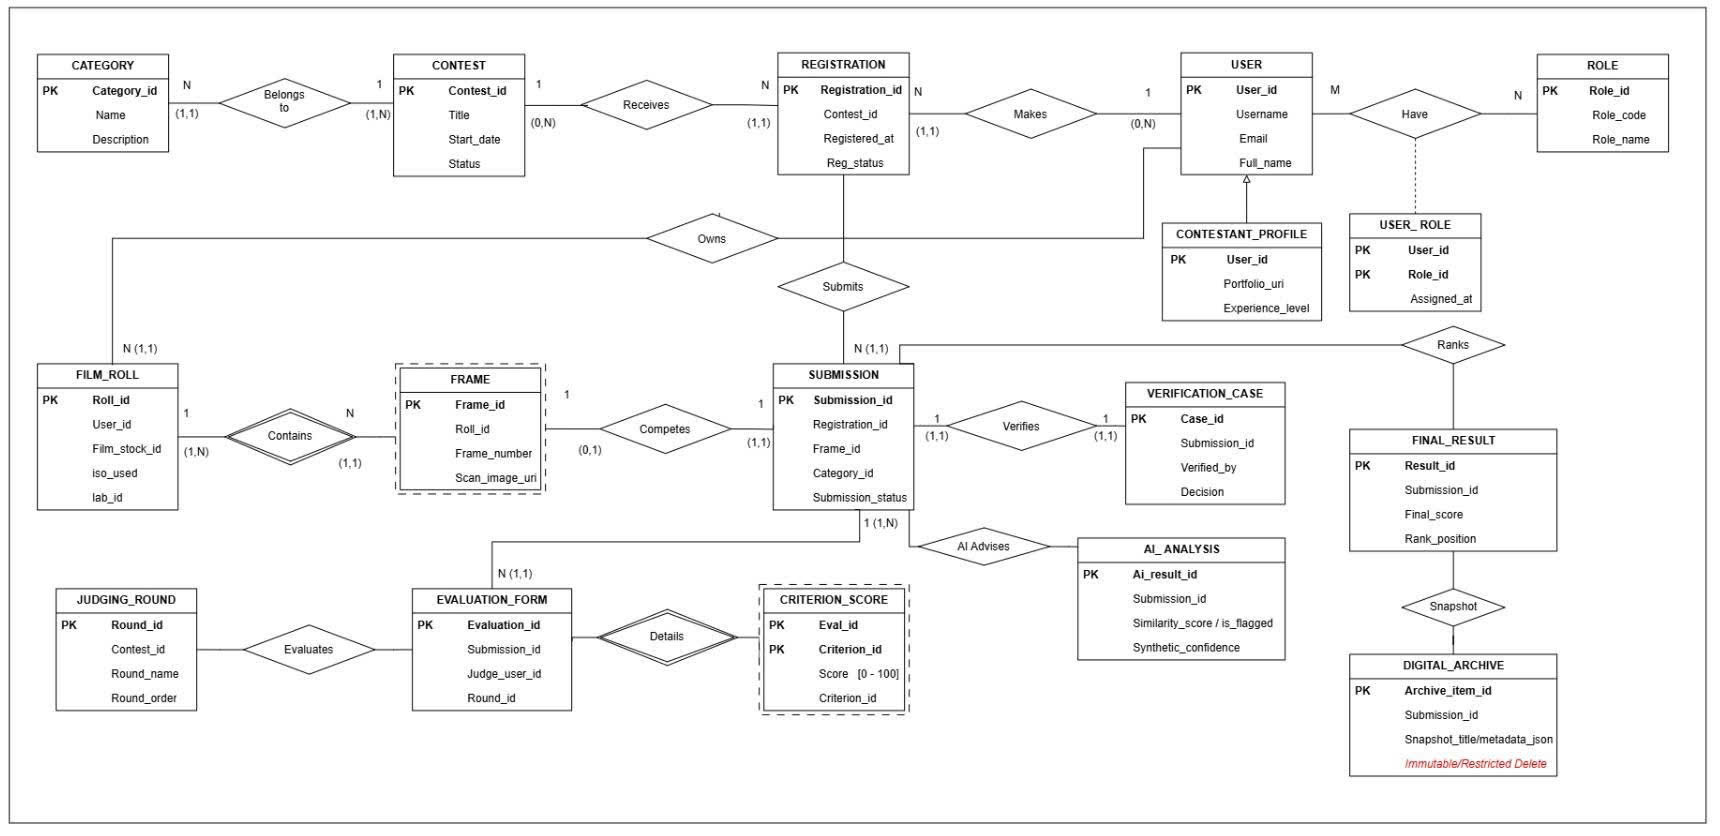
\includegraphics[width=\textwidth,keepaspectratio]{figures/fig_conceptual_erd.png}
    \caption{Sơ đồ Thực thể Liên kết Ý niệm (Conceptual ERD) chuẩn hóa 32 thực thể}
    \label{fig:c4_conceptual_erd}
\end{figure}

% ----------------------------------------------------------------------
\section{Bản số (Cardinality) và Ràng buộc Quan hệ Ý niệm}
\label{s:c4_cardinalities}

Mỗi mối quan hệ được xác lập bằng bản số chuẩn (\textit{Cardinality}):
\begin{itemize}
    \item \textbf{Phân hệ Quản trị Cuộc thi}:
    \begin{itemize}
        \item $\text{Contest } (1,1) \longleftrightarrow (1,N) \text{ ContestCategory}$: Mỗi cuộc thi bắt buộc có ít nhất một hạng mục chuyên môn (BR-O-001).
        \item $\text{Contest } (1,1) \longleftrightarrow (0,N) \text{ Registration}$: Cuộc thi tiếp nhận các đơn đăng ký từ thí sinh.
        \item $\text{Contest } (1,1) \longleftrightarrow (0,N) \text{ Submission}$: Cuộc thi là ngữ cảnh chứa các bài dự thi.
    \end{itemize}
    \item \textbf{Phân hệ Quản lý Người dùng \& Thí sinh}:
    \begin{itemize}
        \item $\text{UserAccount } (1,1) \longleftrightarrow (1,N) \text{ UserRole}$: Một người dùng có thể sở hữu nhiều vai trò khác nhau (BR-P-001).
        \item $\text{UserAccount } (1,1) \longleftrightarrow (0,1) \text{ ParticipantProfile}$: Quan hệ một-một tùy chọn.
    \end{itemize}
    \item \textbf{Phân hệ Xuất xứ Phim Vật lý}:
    \begin{itemize}
        \item $\text{ParticipantProfile } (1,1) \longleftrightarrow (0,N) \text{ FilmRoll}$: Một thí sinh sở hữu nhiều cuộn phim.
        \item $\text{FilmRoll } (1,1) \longleftrightarrow (1,N) \text{ FilmFrame}$: Một cuộn phim chứa nhiều khung hình; một khung hình bắt buộc phải thuộc về đúng một cuộn phim.
        \item $\text{FilmFrame } (1,1) \longleftrightarrow (0,1) \text{ Camera}$: Khung hình ghi nhận thiết bị máy ảnh sử dụng.
        \item $\text{FilmFrame } (1,1) \longleftrightarrow (0,1) \text{ Lens}$: Khung hình ghi nhận ống kính sử dụng.
        \item $\text{FilmRoll } (1,1) \longleftrightarrow (0,1) \text{ Lab}$: Cuộn phim được xử lý tráng tại một phòng lab.
    \end{itemize}
    \item \textbf{Phân hệ Nộp bài \& Thẩm định}:
    \begin{itemize}
        \item $\text{Registration } (1,1) \longleftrightarrow (0,N) \text{ Submission}$: Một đơn đăng ký có thể nộp nhiều bài thi vào các hạng mục cho phép.
        \item $\text{FilmFrame } (1,1) \longleftrightarrow (0,N) \text{ Submission}$: Khung hình được sử dụng làm tác phẩm dự thi.
        \item $\text{Submission } (1,1) \longleftrightarrow (1,1) \text{ VerificationCase}$: Mỗi bài thi có đúng một hồ sơ thẩm định chính thức.
        \item $\text{Submission } (1,1) \longleftrightarrow (0,N) \text{ AIAnalysisResult}$: Một bài thi có thể có nhiều kết quả phân tích từ các mô hình AI khác nhau.
    \end{itemize}
    \item \textbf{Phân hệ Chấm thi \& Tổng kết}:
    \begin{itemize}
        \item $\text{ContestCategory } (1,1) \longleftrightarrow (1,N) \text{ JudgingRound}$: Mỗi hạng mục có ít nhất một vòng chấm thi.
        \item $\text{JudgingRound } (1,1) \longleftrightarrow (1,N) \text{ ScoringCriterion}$: Mỗi vòng có một hoặc nhiều tiêu chí chấm điểm riêng biệt.
        \item $\text{JudgingRound } (1,1) \longleftrightarrow (0,N) \text{ JudgeAssignment}$; \\
        $\text{JudgeAssignment } (1,1) \longleftrightarrow (1,N) \text{ UserAccount (Judge role)}$: Phân công tài khoản người dùng mang vai trò Judge vào vòng thi.
        \item $\text{Evaluation } (1,1) \longleftrightarrow (1,N) \text{ EvaluationScore}$; \\
        $\text{EvaluationScore } (1,1) \longleftrightarrow (1,N) \text{ ScoringCriterion}$: Phiếu chấm chứa điểm chi tiết theo tiêu chí.
        \item $\text{Result } (1,1) \longleftrightarrow (0,N) \text{ AwardAssignment}$; \\
        $\text{AwardAssignment } (1,1) \longleftrightarrow (1,1) \text{ AwardDefinition}$: Gán giải thưởng cho kết quả chung cuộc.
        \item $\text{Result } (1,1) \longleftrightarrow (0,1) \text{ ArchiveItem}$: Chỉ bài thi có kết quả chung cuộc mới được chuyển vào kho lưu trữ số.
    \end{itemize}
    \item \textbf{Phân hệ Mẫu Cấu hình Cuộc thi (Reusable Contest Templates)}:
    \begin{itemize}
        \item $\text{ContestTemplate } (1,1) \longleftrightarrow (1,N) \text{ TemplateCategory}$: Một template chứa ít nhất một hạng mục mẫu.
        \item $\text{TemplateCategory } (1,1) \longleftrightarrow (1,N) \text{ TemplateJudgingRound}$: Mỗi hạng mục mẫu có các vòng chấm mẫu.
        \item $\text{TemplateJudgingRound } (1,1) \longleftrightarrow (1,N) \text{ TemplateScoringCriterion}$: Vòng chấm mẫu định nghĩa các tiêu chí mẫu.
        \item $\text{TemplateCategory } (1,1) \longleftrightarrow (0,N) \text{ TemplateAwardDefinition}$: Định nghĩa cơ cấu giải mẫu theo hạng mục.
        \item $\text{ContestTemplate } (0,1) \longleftrightarrow (0,N) \text{ Contest}$: Cuộc thi có thể được nhân bản tự động từ một template.
    \end{itemize}
    \item \textbf{Phân hệ Siêu dữ liệu Tài sản Số (Structured Digital Asset Metadata)}:
    \begin{itemize}
        \item $\text{Submission } (1,1) \longleftrightarrow (0,1) \text{ AssetMetadata}$: Mỗi bài thi liên kết bản ghi siêu dữ liệu kỹ thuật số hóa chi tiết và bằng chứng kiểm định chất lượng (QC).
    \end{itemize}
\end{itemize}

\subsection{Bảng Đối soát Độ phủ Quan hệ}
Sự phân bổ bản số và đối soát độ phủ quan hệ giữa các luồng nghiệp vụ được trình bày trong Bảng~\ref{tab:c4_relationship_coverage}:

\begin{table}[!ht]
\centering
\caption{Đối soát độ phủ quan hệ giữa luồng nghiệp vụ và mô hình ý niệm}
\label{tab:c4_relationship_coverage}
\small
\begin{tabularx}{\textwidth}{p{2.2cm}p{4.6cm}>{\raggedright\arraybackslash}X}
\toprule
\textbf{Luồng nghiệp vụ} & \textbf{Quan hệ kiểm soát} & \textbf{Quyết định bản số} \\
\midrule
Đăng ký & \texttt{ParticipantProfile}--\texttt{Registration}--\texttt{Contest} & Một đơn thuộc một thí sinh và một cuộc thi. \\
Xuất xứ & \texttt{ParticipantProfile}--\texttt{FilmRoll}--\texttt{FilmFrame} & Một cuộn thuộc một thí sinh và chứa nhiều frame. \\
Nộp bài & \texttt{Registration}--\texttt{Submission}--\texttt{FilmFrame}--\texttt{ContestCategory} & Một bài có một frame; frame có thể tái sử dụng giữa các contest. \\
Thẩm định & \texttt{Submission}--\texttt{VerificationCase}/\allowbreak\texttt{AIAnalysisResult} & Một case người duyệt và nhiều kết quả AI tư vấn. \\
Chấm thi & \texttt{JudgingRound}--\texttt{JudgeAssignment}--\texttt{Evaluation}--\texttt{EvaluationScore} & Mọi đánh giá đều nằm trong một vòng chấm. \\
Kết quả & \texttt{Submission}--\texttt{Result}--\texttt{ArchiveItem} & Result và archive chỉ phát sinh khi đủ điều kiện cuối vòng. \\
\bottomrule
\end{tabularx}
\end{table}

% ----------------------------------------------------------------------
\section{Thiết kế Cấp độ 2: Mô hình Quan hệ Logic và Giải quyết Quan hệ \texorpdfstring{$N:M$}{N:M}}
\label{s:c4_logical_model}

\subsection{Phân loại Quy tắc và Ranh giới Quyết định}
Ranh giới quyết định giữa các quy tắc chính thức và quy tắc đề xuất được phân loại trong Bảng~\ref{tab:c4_rule_boundary}:

\begin{table}[!ht]
\centering
\caption{Phân loại business rule và ranh giới quyết định trong mô hình ý niệm}
\label{tab:c4_rule_boundary}
\small
\begin{tabularx}{\textwidth}{p{2.2cm}>{\raggedright\arraybackslash}Xp{3.2cm}}
\toprule
\textbf{Loại quy tắc} & \textbf{Nội dung ở mức ý niệm} & \textbf{Chủ thể quyết định} \\
\midrule
Chính thức & Submission cần registration hợp lệ, một frame, một category và được con người thẩm định trước khi chấm. & Workflow và Organizer \\
Chính thức & AI chỉ tư vấn, không tự quyết định Verified hoặc Rejected. & Organizer \\
Chính thức & Result và ArchiveItem phản ánh kết quả đã hoàn tất và lịch sử cần bảo tồn. & Organizer và lifecycle \\
Đề xuất & Frame được dùng lại giữa các contest nhưng không lặp trong cùng một contest. & Nhóm thiết kế / chính sách \\
Đề xuất & User có thể giữ nhiều role nhưng vẫn chịu quy tắc xung đột lợi ích. & Nhóm thiết kế / chính sách \\
\bottomrule
\end{tabularx}
\end{table}

Các chi tiết datatype, constraint, index, procedure và trigger không thuộc mô hình ý niệm; chúng được chuyển sang các cấp độ thiết kế sau.

Khi chuyển đổi từ mô hình ý niệm sang mô hình quan hệ logic, các quan hệ Nhiều-Nhiều ($N:M$) được giải quyết triệt để thông qua các quan hệ kết hợp (\textit{Associative Relations}) được tổng hợp trong Bảng~\ref{tab:c4_nm_resolution}:

\begin{table}[!ht]
\centering
\caption{Giải quyết các quan hệ Nhiều-Nhiều trong mô hình logic}
\label{tab:c4_nm_resolution}
\scriptsize
\begin{tabularx}{\textwidth}{p{3.8cm}p{3.2cm}>{\raggedright\arraybackslash}X}
\toprule
\textbf{Quan hệ Ý niệm $N:M$} & \textbf{Quan hệ Kết hợp Logic} & \textbf{Thuộc tính mở rộng / Khóa thay thế} \\
\midrule
UserAccount $\leftrightarrow$ Role & \texttt{UserRole} & \texttt{user\_id}, \texttt{role\_id}, \texttt{assigned\_at}, \texttt{status} \\
JudgingRound $\leftrightarrow$ UserAccount (Judge role) & \texttt{JudgeAssignment} & \texttt{round\_id}, \texttt{judge\_user\_id}, \texttt{assigned\_at} \\
Evaluation $\leftrightarrow$ ScoringCriterion & \texttt{EvaluationScore} & \texttt{evaluation\_id}, \texttt{criterion\_id}, \texttt{score\_value}, \texttt{comment} \\
Result $\leftrightarrow$ AwardDefinition & \texttt{AwardAssignment} & \texttt{result\_id}, \texttt{award\_definition\_id}, \texttt{assigned\_at} \\
\bottomrule
\end{tabularx}
\end{table}

\paragraph{Danh mục Khóa Dự tuyển và Khóa Thay thế (Candidate \& Alternate Keys)}
Mỗi quan hệ logic sử dụng khóa thay thế nhân tạo (\textit{Surrogate Primary Key}, ví dụ: \texttt{submission\_id}) để tối ưu hiệu năng liên kết bảng, đồng thời bắt buộc thiết lập các khóa thay thế tự nhiên (\textit{Natural Alternate Keys}) để bảo vệ tính duy nhất nghiệp vụ:
\begin{itemize}
    \item \texttt{UserAccount}: \texttt{email} (UNIQUE), \texttt{username} (UNIQUE).
    \item \texttt{Contest}: \texttt{contest\_code} (UNIQUE).
    \item \texttt{ContestCategory}: \texttt{(contest\_id, category\_code)} (UNIQUE Composite).
    \item \texttt{FilmRoll}: \texttt{(participant\_id, roll\_code)} (UNIQUE Composite).
    \item \texttt{FilmFrame}: \texttt{(roll\_id, frame\_number)} (UNIQUE Composite).
    \item \texttt{Registration}: \texttt{(contest\_id, participant\_id)} (UNIQUE Composite).
    \item \texttt{Submission}: \texttt{(contest\_id, frame\_id)} (UNIQUE Composite -- BR-P-006).
    \item \texttt{JudgeAssignment}: \texttt{(round\_id, judge\_user\_id)} (UNIQUE Composite).
    \item \texttt{Evaluation}: \texttt{(round\_id, submission\_id, judge\_user\_id)} (UNIQUE Composite -- BR-O-009).
    \item \texttt{EvaluationScore}: \texttt{(evaluation\_id, criterion\_id)} (UNIQUE Composite).
    \item \texttt{Result}: \texttt{(category\_id, submission\_id)} (UNIQUE Composite).
    \item \texttt{ContestTemplate}: \texttt{template\_code} (UNIQUE).
    \item \texttt{TemplateCategory}: \texttt{(template\_id, category\_code)} (UNIQUE Composite).
    \item \texttt{TemplateJudgingRound}: \texttt{(template\_category\_id, round\_number)} (UNIQUE Composite).
    \item \texttt{TemplateScoringCriterion}: \texttt{(template\_round\_id, criterion\_code)} (UNIQUE Composite).
    \item \texttt{TemplateAwardDefinition}: \texttt{(template\_category\_id, award\_code)} (UNIQUE Composite).
    \item \texttt{AssetMetadata}: \texttt{submission\_id} (UNIQUE Composite -- 1:1), \texttt{checksum\_sha256} (INDEX).
\end{itemize}

Mô hình quan hệ logic đạt chuẩn 3NF sau khi giải quyết các quan hệ Nhiều-Nhiều được thể hiện chi tiết trong Hình~\ref{fig:c4_logical_erd}:

\begin{figure}[!ht]
    \centering
    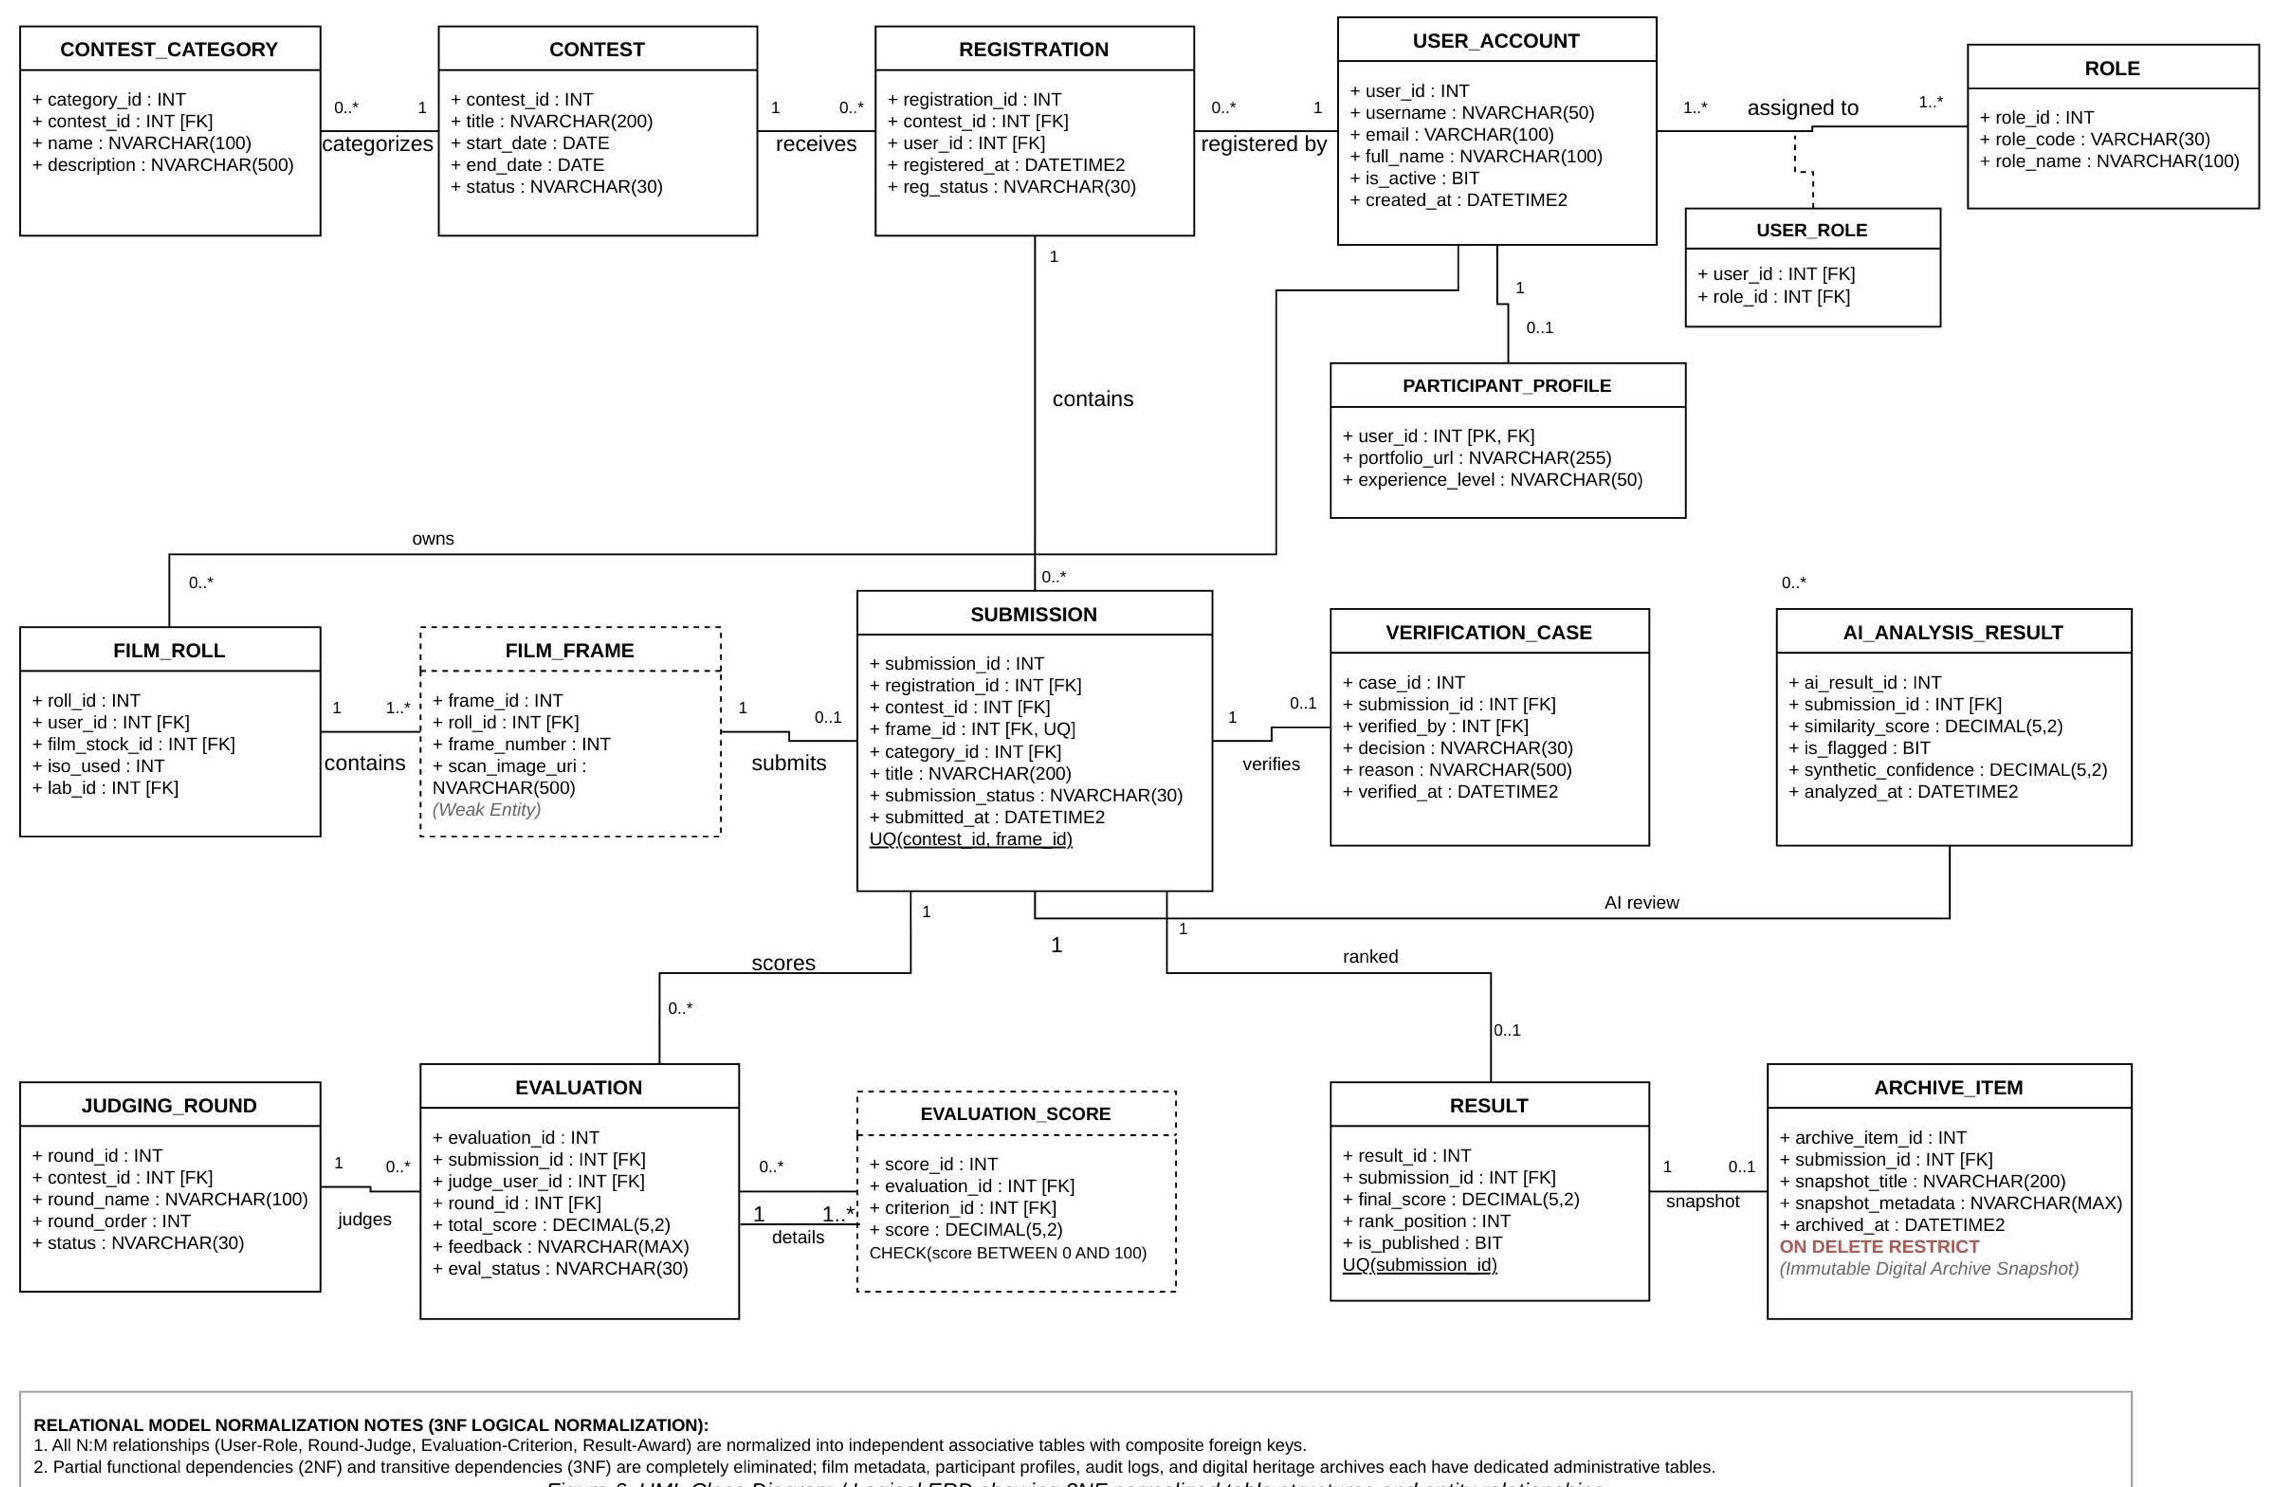
\includegraphics[width=\textwidth,keepaspectratio]{figures/fig_logical_erd.png}
    \caption{Sơ đồ Lớp / Mô hình Quan hệ Logic (Logical Schema / UML Class Diagram) đạt chuẩn 3NF}
    \label{fig:c4_logical_erd}
\end{figure}

% ----------------------------------------------------------------------
\section{Chứng minh Chuẩn hóa Dữ liệu (Normalization Proof to 3NF)}
\label{s:c4_normalization}

Để chứng minh tính đúng đắn khoa học, các quan hệ trọng yếu trong hệ thống được phân tích phụ thuộc hàm (\textit{Functional Dependencies - FD}) và chứng minh đạt dạng chuẩn 3 (3NF):

\subsection{Quan hệ FilmFrame (Khung hình phim)}
\begin{itemize}
    \item \textbf{Tập thuộc tính}: 
    \begin{center}
    $\text{FilmFrame}(\underline{\text{frame\_id}}, \text{roll\_id}, \text{camera\_id}, \text{lens\_id}, \text{frame\_number},$ \\
    $\text{frame\_title}, \text{captured\_on}, \text{capture\_location}, \text{frame\_status}, \text{negative\_uri})$
    \end{center}
    \item \textbf{Phụ thuộc hàm cốt lõi}:
    \begin{align*}
        \text{FD1: } & \text{frame\_id} \longrightarrow \{\text{roll\_id}, \text{camera\_id}, \text{lens\_id}, \\
        & \phantom{\text{frame\_id} \longrightarrow \{} \text{frame\_number}, \text{frame\_title}, \text{captured\_on}, \\
        & \phantom{\text{frame\_id} \longrightarrow \{} \text{capture\_location}, \text{frame\_status}, \text{negative\_uri}\} \\
        \text{FD2: } & (\text{roll\_id}, \text{frame\_number}) \longrightarrow \{\text{frame\_id}, \text{camera\_id}, \text{lens\_id}, \\
        & \phantom{(\text{roll\_id}, \text{frame\_number}) \longrightarrow \{} \text{frame\_title}, \text{captured\_on}, \text{capture\_location}, \\
        & \phantom{(\text{roll\_id}, \text{frame\_number}) \longrightarrow \{} \text{frame\_status}, \text{negative\_uri}\}
    \end{align*}
    \item \textbf{Chứng minh 1NF}: Mọi thuộc tính đều mang giá trị nguyên tố (\textit{atomic}), không có thuộc tính lặp hay đa trị.
    \item \textbf{Chứng minh 2NF}: Khóa chính \texttt{frame\_id} gồm 1 thuộc tính đơn lẻ, do đó không tồn tại phụ thuộc hàm bộ phận vào một phần của khóa.
    \item \textbf{Chứng minh 3NF}: Không tồn tại phụ thuộc bắc cầu giữa các thuộc tính không khóa. Thông tin về thân máy (\texttt{Camera}) và ống kính (\texttt{Lens}) đã được tách thành các quan hệ tham chiếu riêng, chỉ lưu trữ khóa ngoại tại bảng \texttt{FilmFrame}. $\Rightarrow$ \textbf{Đạt 3NF}.
\end{itemize}

\subsection{Quan hệ Submission (Bài dự thi)}
\begin{itemize}
    \item \textbf{Tập thuộc tính}: 
    \begin{center}
    $\text{Submission}(\underline{\text{submission\_id}}, \text{registration\_id}, \text{contest\_id}, \text{category\_id},$ \\
    $\text{frame\_id}, \text{submission\_title}, \text{statement}, \text{image\_uri}, \text{submitted\_at}, \text{status})$
    \end{center}
    \item \textbf{Phụ thuộc hàm cốt lõi}:
    \begin{align*}
        \text{FD1: } & \text{submission\_id} \longrightarrow \{\text{registration\_id}, \text{contest\_id}, \text{category\_id}, \\
        & \phantom{\text{submission\_id} \longrightarrow \{} \text{frame\_id}, \text{submission\_title}, \text{statement}, \\
        & \phantom{\text{submission\_id} \longrightarrow \{} \text{image\_uri}, \text{submitted\_at}, \text{status}\} \\
        \text{FD2: } & (\text{contest\_id}, \text{frame\_id}) \longrightarrow \{\text{submission\_id}, \text{registration\_id}, \\
        & \phantom{(\text{contest\_id}, \text{frame\_id}) \longrightarrow \{} \text{category\_id}, \text{submission\_title}, \\
        & \phantom{(\text{contest\_id}, \text{frame\_id}) \longrightarrow \{} \text{statement}, \text{image\_uri}, \text{submitted\_at}, \text{status}\}
    \end{align*}
    \item \textbf{Chứng minh 3NF}: Không lưu trữ lặp lại thông tin tên thí sinh hay tên cuộc thi trong bảng \texttt{Submission}. Mọi thông tin danh tính đều được truy xuất qua \texttt{registration\_id} và \texttt{frame\_id}. Không có phụ thuộc hàm giữa các thuộc tính không khóa. $\Rightarrow$ \textbf{Đạt 3NF}.
\end{itemize}

\subsection{Quan hệ EvaluationScore (Điểm tiêu chí đánh giá)}
\begin{itemize}
    \item \textbf{Tập thuộc tính}:
    \begin{center}
    $\text{EvaluationScore}(\underline{\text{evaluation\_score\_id}}, \text{evaluation\_id},$ \\
    $\text{criterion\_id}, \text{score\_value}, \text{score\_comment})$
    \end{center}
    \item \textbf{Phụ thuộc hàm cốt lõi}:
    \begin{align*}
        \text{FD1: } & \text{evaluation\_score\_id} \longrightarrow \{\text{evaluation\_id}, \text{criterion\_id}, \\
        & \phantom{\text{evaluation\_score\_id} \longrightarrow \{} \text{score\_value}, \text{score\_comment}\} \\
        \text{FD2: } & (\text{evaluation\_id}, \text{criterion\_id}) \longrightarrow \{\text{evaluation\_score\_id}, \\
        & \phantom{(\text{evaluation\_id}, \text{criterion\_id}) \longrightarrow \{} \text{score\_value}, \text{score\_comment}\}
    \end{align*}
    \item \textbf{Chứng minh 3NF}: Tên tiêu chí, thang điểm min/max và trọng số được lưu tại \texttt{ScoringCriterion}, không bị lặp lại trong \texttt{EvaluationScore}. Bảng chỉ lưu giá trị điểm và nhận xét ứng với từng tiêu chí cụ thể. $\Rightarrow$ \textbf{Đạt 3NF}.
\end{itemize}

\subsection{Quan hệ Result (Kết quả Xếp hạng và Công bố)}
\begin{itemize}
    \item \textbf{Tập thuộc tính}:
    \begin{center}
    $\text{Result}(\underline{\text{result\_id}}, \text{category\_id}, \text{submission\_id}, \text{final\_score}, \text{final\_rank},$ \\
    $\text{result\_status}, \text{tie\_break\_note}, \text{finalized\_at}, \text{finalized\_by\_user\_id}, \text{published\_at})$
    \end{center}
    \item \textbf{Phụ thuộc hàm cốt lõi}:
    \begin{align*}
        \text{FD1: } & \text{result\_id} \longrightarrow \{\text{category\_id}, \text{submission\_id}, \text{final\_score}, \text{final\_rank}, \\
        & \qquad \text{result\_status}, \text{tie\_break\_note}, \text{finalized\_at}, \\
        & \qquad \text{finalized\_by\_user\_id}, \text{published\_at}\} \\
        \text{FD2: } & (\text{category\_id}, \text{submission\_id}) \longrightarrow \{\text{result\_id}, \text{final\_score}, \text{final\_rank}, \\
        & \qquad \text{result\_status}, \text{tie\_break\_note}, \text{finalized\_at}, \\
        & \qquad \text{finalized\_by\_user\_id}, \text{published\_at}\}
    \end{align*}
    \item \textbf{Chứng minh 3NF}: Không lưu trữ lặp lại thông tin thí sinh, cuộn phim hay tên hạng mục trong bảng \texttt{Result}. Toàn bộ thông tin ngữ cảnh được truy xuất gián tiếp qua khóa ngoại \texttt{category\_id} và \texttt{submission\_id}. Ý nghĩa của kết quả phụ thuộc hàm đầy đủ vào cặp thực thể (\texttt{category\_id}, \texttt{submission\_id}). $\Rightarrow$ \textbf{Đạt 3NF}.
\end{itemize}

% ----------------------------------------------------------------------
\section{Chiến lược Phi Chuẩn hóa có Kiểm soát cho Kho Lưu trữ Số}
\label{s:c4_archive_denormalization}

Quan hệ \texttt{ArchiveItem} là trường hợp ngoại lệ duy nhất được cố tình thiết kế theo hướng \textbf{Phi chuẩn hóa có kiểm soát (\textit{Controlled Denormalization})}:

\begin{itemize}
    \item Thay vì chỉ lưu trữ các khóa ngoại sống (\texttt{result\_id}, \texttt{submission\_id}) trỏ về các bảng giao dịch, \texttt{ArchiveItem} lưu trữ các bản chụp JSON bất biến: \texttt{contest\_snapshot}, \texttt{category\_snapshot}, \texttt{participant\_snapshot}, \texttt{technical\_snapshot}, \texttt{judging\_snapshot}.
    \item \textbf{Căn cứ lý thuyết \& Thực tiễn}: Kho lưu trữ di sản số có mục đích bảo tồn nguyên trạng giá trị lịch sử tại thời điểm trao giải. Nếu trong tương lai tài khoản thí sinh đổi tên, hoặc cấu hình cuộc thi gốc bị điều chỉnh/ẩn đi, tác phẩm trong kho lưu trữ di sản vẫn giữ nguyên 100\% thông tin trung thực của thời điểm đoạt giải mà không bị sai lệch.
\end{itemize}

% ----------------------------------------------------------------------
\section{Từ điển Dữ liệu Logic (Logical Data Dictionary)}
\label{s:c4_data_dictionary}

Bảng~\ref{tab:c4_data_dictionary} hệ thống hóa từ điển dữ liệu logic cho các thuộc tính nghiệp vụ cốt lõi, xác lập rõ ranh giới ngữ nghĩa và vòng đời dữ liệu giữa các phân hệ:

\begin{table}[!ht]
\centering
\caption{Từ điển dữ liệu logic cho các thực thể và thuộc tính trọng yếu}
\label{tab:c4_data_dictionary}
\footnotesize
\begin{tabularx}{\textwidth}{>{\bfseries\raggedright\arraybackslash}p{4.2cm}>{\raggedright\arraybackslash}X>{\raggedright\arraybackslash}p{2.8cm}}
\toprule
\textbf{Thực thể.Thuộc tính} & \textbf{Ý nghĩa nghiệp vụ \& Ràng buộc logic} & \textbf{Miền giá trị / Quy ước} \\
\midrule
UserAccount.\allowbreak email & Địa chỉ email duy nhất dùng đăng nhập hệ thống & Duy nhất (UNIQUE), hợp lệ \\
Role.\allowbreak role\_code & Mã vai trò kiểm soát truy cập (RBAC) & ADMIN, ORGANIZER, \allowbreak JUDGE, PARTICIPANT \\
ParticipantProfile.\allowbreak status & Trạng thái hoạt động của hồ sơ thí sinh & ACTIVE, INACTIVE, \allowbreak SUSPENDED \\
Contest.\allowbreak contest\_code & Mã định danh nghiệp vụ của cuộc thi & Duy nhất toàn hệ thống \\
Contest.\allowbreak contest\_status & Vòng đời tổ chức của cuộc thi & DRAFT, PUBLISHED, \allowbreak OPEN, CLOSED, \allowbreak FINALIZED, ARCHIVED \\
ContestCategory.\allowbreak category\_code & Mã hạng mục chuyên môn trong cuộc thi & Duy nhất trong phạm vi contest \\
JudgingRound.\allowbreak is\_final\_round & Cờ đánh dấu vòng chấm chung khảo quyết định giải & TRUE / FALSE \\
ScoringCriterion.\allowbreak weight\_percent & Trọng số đóng góp của tiêu chí vào điểm tổng & $0 < \text{weight} \leq 100$ \\
FilmFrame.\allowbreak frame\_number & Số thứ tự khung hình trên cuộn phim vật lý & Duy nhất theo từng roll\_id \\
Submission.\allowbreak submission\_status & Trạng thái xử lý bài thi qua các giai đoạn & PENDING\_VERIFICATION, \allowbreak VERIFIED, REJECTED, \allowbreak JUDGED, FINALIZED \\
VerificationCase.\allowbreak final\_decision & Quyết định thẩm định chính thức của con người & VERIFIED, REJECTED, \allowbreak NEEDS\_CLARIFICATION \\
AIAnalysisResult.\allowbreak confidence & Điểm số tin cậy do mô hình AI trả về & $0.0000 \leq \text{conf} \leq 1.0000$ \\
JudgeAssignment.\allowbreak status & Tình trạng nhận việc của giám khảo trong vòng & ASSIGNED, IN\_PROGRESS, \allowbreak SUBMITTED, CANCELLED \\
Evaluation.\allowbreak total\_score & Tổng điểm có trọng số của một giám khảo & Tổng điểm hợp lệ $\geq 0$ \\
Result.\allowbreak final\_rank & Thứ hạng chung cuộc của bài thi trong hạng mục & Số nguyên dương $\geq 1$ \\
ArchiveItem.\allowbreak contest\_snapshot & Bản chụp bất biến của cuộc thi tại thời điểm trao giải & Định dạng JSON cấu trúc \\
AuditLog.\allowbreak action\_code & Mã định danh hành động nghiệp vụ cần kiểm toán & INSERT, UPDATE, \allowbreak STATUS\_CHANGE \\
ContestTemplate.\allowbreak template\_code & Mã định danh duy nhất của mẫu cấu hình cuộc thi & Duy nhất (UNIQUE), hợp lệ \\
AssetMetadata.\allowbreak checksum\_sha256 & Mã băm SHA-256 64 ký tự hex kiểm tra toàn vẹn tệp & Đúng 64 ký tự hex hợp lệ \\
AssetMetadata.\allowbreak qc\_status & Kết quả kiểm tra chất lượng số hóa tệp ảnh scan & PASSED, FAILED, \allowbreak FLAGGED, PENDING \\
\bottomrule
\end{tabularx}
\end{table}

% ----------------------------------------------------------------------
\section{Vòng đời Trạng thái của các Thực thể Cốt lõi (Entity Lifecycle)}
\label{s:c4_lifecycles}

Sự vận hành của cơ sở dữ liệu được định hướng bởi các máy trạng thái hữu hạn (\textit{Finite State Machines}) chặt chẽ. Bảng~\ref{tab:c4_lifecycles} tổng kết chuỗi chuyển đổi trạng thái hợp lệ của các thực thể trung tâm:

\begin{table}[!ht]
\centering
\caption{Tổng hợp vòng đời trạng thái của các thực thể cốt lõi trong hệ thống}
\label{tab:c4_lifecycles}
\small
\begin{tabularx}{\textwidth}{>{\bfseries}p{3.2cm}>{\raggedright\arraybackslash}X}
\toprule
\textbf{Thực thể} & \textbf{Chuỗi chuyển đổi trạng thái vòng đời chuẩn} \\
\midrule
Contest & \texttt{DRAFT} $\rightarrow$ \texttt{PUBLISHED} $\rightarrow$ \texttt{OPEN} $\rightarrow$ \texttt{CLOSED} $\rightarrow$ \texttt{FINALIZED} $\rightarrow$ \texttt{ARCHIVED} \\
Registration & \texttt{PENDING} $\rightarrow$ \texttt{APPROVED} / \texttt{REJECTED} / \texttt{WITHDRAWN} \\
FilmRoll & \texttt{DRAFT} $\rightarrow$ \texttt{READY} $\rightarrow$ \texttt{ARCHIVED} \\
FilmFrame & \texttt{DRAFT} $\rightarrow$ \texttt{READY} $\rightarrow$ \texttt{SUBMITTED} $\rightarrow$ \texttt{ARCHIVED} \\
Submission & \texttt{DRAFT} $\rightarrow$ \texttt{PENDING\_VERIFICATION} $\rightarrow$ \texttt{VERIFIED} / \texttt{REJECTED} / \\
 & \texttt{NEEDS\_CLARIFICATION} $\rightarrow$ \texttt{JUDGED} $\rightarrow$ \texttt{FINALIZED} $\rightarrow$ \texttt{ARCHIVED} \\
VerificationCase & \texttt{PENDING} $\rightarrow$ \texttt{UNDER\_REVIEW} $\rightarrow$ \texttt{VERIFIED} / \texttt{REJECTED} / \texttt{NEEDS\_CLARIFICATION} \\
JudgeAssignment & \texttt{ASSIGNED} $\rightarrow$ \texttt{IN\_PROGRESS} $\rightarrow$ \texttt{SUBMITTED} / \texttt{CANCELLED} \\
Evaluation & \texttt{DRAFT} $\rightarrow$ \texttt{SUBMITTED} $\rightarrow$ \texttt{LOCKED} \\
Result & \texttt{DRAFT} $\rightarrow$ \texttt{FINALIZED} $\rightarrow$ \texttt{PUBLISHED} \\
ArchiveItem & \texttt{PENDING\_ARCHIVE} $\rightarrow$ \texttt{ARCHIVED} $\rightarrow$ \texttt{RETIRED} \\
\bottomrule
\end{tabularx}
\end{table}


\chapter{Thiết kế CSDL cấp độ 3: Mô hình vật lý và lập trình CSDL}\label{c:physical_implementation}
% Chapter 5: Thiết kế CSDL Cấp độ 3: Mô hình Vật lý và Lập trình CSDL

Chương này trình bày chi tiết cấp độ thiết kế vật lý (\textit{Physical Database Design}) và hiện thực hóa lập trình cơ sở dữ liệu trên hệ quản trị Microsoft SQL Server. Toàn bộ lược đồ vật lý được cấu trúc hóa theo các schema nghiệp vụ, thiết lập hệ thống ràng buộc toàn vẹn nghiêm ngặt, chiến lược đánh chỉ mục (\textit{Indexing}) tối ưu theo các mẫu truy vấn thực tế, cùng hệ thống Views, Stored Procedures và Triggers bảo đảm an toàn giao dịch.

% ----------------------------------------------------------------------
\section{Lựa chọn Hệ Quản trị và Quy ước Đặt tên Vật lý}
\label{s:c5_dbms_naming}

\subsection{Căn cứ Lựa chọn Microsoft SQL Server}
Hệ quản trị cơ sở dữ liệu Microsoft SQL Server (bản 2022+ chạy trên Linux Container) được lựa chọn chính thức dựa trên các căn cứ kỹ thuật:
\begin{enumerate}
    \item \textbf{Cơ chế thực thi ràng buộc toàn vẹn mạnh mẽ}: Hỗ trợ đầy đủ các ràng buộc phức tạp (\texttt{CHECK}, \texttt{UNIQUE}, \texttt{FOREIGN KEY}) với độ tin cậy giao dịch ACID tuyệt đối.
    \item \textbf{Khả năng mở rộng và lập trình T-SQL phong phú}: Ngôn ngữ T-SQL hỗ trợ mạnh mẽ việc đóng gói logic nghiệp vụ vào Stored Procedures và Triggers.
    \item \textbf{Tương thích hoàn hảo với công cụ quản trị}: Khả năng kết nối, giám sát và kiểm thử trực quan thông qua SQL Server Management Studio (SSMS 22).
\end{enumerate}

\subsection{Quy ước Đặt tên Đối tượng Vật lý (Naming Conventions)}
Để đảm bảo tính chuyên nghiệp và đồng bộ, toàn bộ đối tượng CSDL tuân thủ quy tắc đặt tên tại Bảng~\ref{tab:c5_naming}:

\begin{table}[htbp]
\centering
\footnotesize
\begin{tabularx}{\textwidth}{>{\bfseries}p{3.0cm}p{4.2cm}>{\raggedright\arraybackslash}X}
\toprule
\textbf{Loại đối tượng} & \textbf{Quy ước đặt tên} & \textbf{Ví dụ minh họa} \\
\midrule
Schema & Chữ thường, danh từ số ít theo module & \texttt{iam}, \texttt{contest}, \texttt{submission} \\
Bảng (Table) & PascalCase, danh từ & \texttt{UserAccount}, \texttt{FilmFrame}, \texttt{Submission} \\
Cột (Column) & snake\_case, rõ nghĩa & \texttt{user\_id}, \texttt{contest\_code}, \texttt{submitted\_at} \\
Khóa chính (PK) & \texttt{PK\_<Schema>\_<Table>} & \texttt{PK\_submission\_Submission} \\
Khóa ngoại (FK) & \texttt{FK\_<Schema>\_<Table>\_<Ref>} & \texttt{FK\_submission\_Submission\_Contest} \\
Duy nhất (UNIQUE) & \texttt{UQ\_<Schema>\_<Table>\_<Cols>} & \texttt{UQ\_submission\_Submission\_contest\_frame} \\
Miền giá trị (CHECK) & \texttt{CK\_<Schema>\_<Table>\_<Rule>} & \texttt{CK\_judging\_Evaluation\_total\_score} \\
Giá trị mặc định (DF) & \texttt{DF\_<Schema>\_<Table>\_<Col>} & \texttt{DF\_iam\_UserAccount\_created\_at} \\
Chỉ mục (Index) & \texttt{IX\_<Schema>\_<Table>\_<Cols>} & \texttt{IX\_submission\_Submission\_contest\_status} \\
View & Schema \texttt{reporting}, tiền tố \texttt{vw\_} & \texttt{reporting.vw\_submission\_overview} \\
Stored Procedure & Schema module, tiền tố \texttt{usp\_} & \texttt{submission.usp\_create\_submission} \\
Trigger & \texttt{TR\_<Schema>\_<Table>\_<Event>} & \texttt{TR\_judging\_EvaluationScore\_AIU} \\
\bottomrule
\end{tabularx}
\caption{Quy ước đặt tên đối tượng cơ sở dữ liệu vật lý}
\label{tab:c5_naming}
\end{table}

% ----------------------------------------------------------------------
\section{Kiến trúc Phân vùng Schema và Lược đồ Bảng}
\label{s:c5_schemas}

Cơ sở dữ liệu được phân chia thành 12 Schema chuyên biệt nhằm phân định ranh giới bảo mật và quản trị:
\begin{itemize}
    \item \texttt{iam}: \texttt{UserAccount}, \texttt{Role}, \texttt{UserRole}.
    \item \texttt{participant}: \texttt{ParticipantProfile}, \texttt{Registration}.
    \item \texttt{reference}: \texttt{FilmStock}, \texttt{Camera}, \texttt{Lens}, \texttt{Lab}.
    \item \texttt{contest}: \texttt{Contest}, \texttt{ContestCategory}, \texttt{JudgingRound}, \texttt{ScoringCriterion}, \texttt{AwardDefinition}, \texttt{ContestTemplate}, \texttt{TemplateCategory}, \texttt{TemplateJudgingRound}, \texttt{TemplateScoringCriterion}, \texttt{TemplateAwardDefinition}.
    \item \texttt{film}: \texttt{FilmRoll}, \texttt{FilmFrame}, \texttt{AssetMetadata}.
    \item \texttt{submission}: \texttt{Submission}.
    \item \texttt{verification}: \texttt{VerificationCase}, \texttt{AIAnalysisResult}.
    \item \texttt{judging}: \texttt{JudgeAssignment}, \texttt{Evaluation}, \texttt{EvaluationScore}.
    \item \texttt{result}: \texttt{Result}, \texttt{AwardAssignment}.
    \item \texttt{archive}: \texttt{ArchiveItem}.
    \item \texttt{audit}: \texttt{AuditLog}.
    \item \texttt{reporting}: Chứa 5 khung nhìn báo cáo (\textit{Views}).
\end{itemize}

\begin{figure}[htbp]
    \centering
    
\includegraphics[width=\textwidth,keepaspectratio]{figures/fig_physical_pdm.png}
    \caption{Sơ đồ Vật lý Cơ sở Dữ liệu (Physical Database Diagram - PDM) trên Microsoft SQL Server 2022 gồm 32 bảng quan hệ}
    \label{fig:c5_physical_pdm}
\end{figure}

% ----------------------------------------------------------------------
\section{Chiến lược Kiểu Dữ liệu Vật lý (Physical Datatype Strategy)}
\label{s:c5_datatypes}

Hệ thống tránh việc sử dụng tùy tiện kiểu \texttt{VARCHAR(255)} cho mọi cột, thay vào đó áp dụng chiến lược lựa chọn kiểu dữ liệu tối ưu cho bộ nhớ và tính chính xác:

\begin{table}[htbp]
\centering
\small
\begin{tabularx}{\textwidth}{p{3.2cm}p{3.6cm}>{\raggedright\arraybackslash}X}
\toprule
\textbf{Mục đích sử dụng} & \textbf{Kiểu dữ liệu SQL Server} & \textbf{Giải thích kỹ thuật} \\
\midrule
Khóa chính nhân tạo & \texttt{INT IDENTITY(1,1)} & Tiết kiệm bộ nhớ (4 bytes), tăng tốc độ nối bảng (JOIN). \\
Mã nghiệp vụ ngắn & \texttt{NVARCHAR(30)} -- \texttt{NVARCHAR(50)} & Đủ chứa mã định danh, kiểm soát độ dài. \\
Tiêu đề / Họ tên & \texttt{NVARCHAR(100)} -- \texttt{NVARCHAR(200)} & Hỗ trợ Unicode đa ngôn ngữ (tiếng Việt có dấu). \\
Văn bản dài / Ghi chú & \texttt{NVARCHAR(1000)} / \texttt{NVARCHAR(MAX)} & Lưu trữ lời tựa nghệ thuật và nhận xét chuyên môn. \\
Mã trạng thái & \texttt{NVARCHAR(30)} & Dễ đọc hiểu khi truy vấn, kiểm soát qua CHECK constraint. \\
Đường dẫn URI ảnh & \texttt{NVARCHAR(500)} & Đủ dung lượng lưu trữ URL Object Storage và mã băm. \\
Điểm số / Trọng số & \texttt{DECIMAL(5,2)} / \texttt{DECIMAL(6,2)} & Độ chính xác số học tuyệt đối, tránh sai số số thực. \\
Độ tin cậy AI & \texttt{DECIMAL(5,4)} & Lưu trữ chính xác giá trị xác suất từ 0.0000 đến 1.0000. \\
Thời gian giao dịch & \texttt{DATETIME2(0)} & Tiết kiệm dung lượng (6 bytes), độ chính xác đến giây. \\
Bản chụp Snapshot & \texttt{NVARCHAR(MAX)} & Lưu trữ cấu trúc JSON bản chụp lịch sử di sản số. \\
\bottomrule
\end{tabularx}
\caption{Chiến lược ánh xạ kiểu dữ liệu trên Microsoft SQL Server}
\label{tab:c5_datatypes}
\end{table}

% ----------------------------------------------------------------------
\section{Thiết kế Ràng buộc Toàn vẹn và Chính sách Khóa Ngoại}
\label{s:c5_constraints}

\paragraph{Chính sách Khóa ngoại và Hành vi Xóa (Referential Action Policy)}
Trong hệ thống quản lý cuộc thi và lưu trữ di sản nghệ thuật, việc bảo toàn dữ liệu lịch sử là yêu cầu sống còn. Do đó, hệ thống áp dụng nguyên tắc:
\begin{itemize}
    \item \textbf{Tuyệt đối không sử dụng \texttt{ON DELETE CASCADE}} đối với các bảng giao dịch trọng yếu (\texttt{Submission}, \texttt{Evaluation}, \texttt{Result}, \texttt{ArchiveItem}). Mọi liên kết khóa ngoại đều thiết lập \texttt{ON DELETE NO ACTION} (mặc định của SQL Server) để ngăn chặn việc vô tình xóa dây chuyền phá hủy dữ liệu lịch sử cuộc thi.
    \item Mọi hoạt động chấm dứt hoặc đóng cuộc thi đều thực hiện thông qua \textbf{chuyển đổi trạng thái nghiệp vụ (\textit{Soft Status Transition})}, không xóa vật lý bản ghi.
\end{itemize}

\paragraph{Ràng buộc Miền giá trị (Check Constraints)}
Hệ thống cài đặt các ràng buộc kiểm tra giá trị toán học, logic thời gian và định dạng kỹ thuật:
\begin{itemize}
    \item \texttt{CK\_contest\_Contest\_dates}: \texttt{registration\_open\_at} $\leq$ \texttt{registration\_close\_at} và \texttt{submission\_open\_at} $\leq$ \texttt{submission\_close\_at}.
    \item \texttt{CK\_contest\_ScoringCriterion\_weight}: \texttt{weight\_percent} $>$ 0 và \texttt{weight\_percent} $\leq$ 100.
    \item \texttt{CK\_contest\_ScoringCriterion\_score\_range}: \texttt{score\_min\_value} $\leq$ \texttt{score\_max\_value}.
    \item \texttt{CK\_verification\_AIAnalysisResult\_confidence}: \texttt{confidence\_score} $\geq$ 0 và \texttt{confidence\_score} $\leq$ 1.
    \item \texttt{CK\_judging\_Evaluation\_total\_score}: \texttt{total\_score} $\geq$ 0.
    \item \texttt{CK\_film\_AssetMetadata\_sha256}: \texttt{LEN(checksum\_sha256) = 64} và không chứa ký tự ngoài tập hex hợp lệ (\texttt{0-9, a-f, A-F}).
    \item \texttt{CK\_film\_AssetMetadata\_bit\_depth}: \texttt{bit\_depth IN (8, 12, 14, 16)}.
    \item \texttt{CK\_film\_AssetMetadata\_qc\_status}: \texttt{qc\_status IN ('PENDING', 'PASSED', 'FAILED', 'FLAGGED')}.
\end{itemize}

% ----------------------------------------------------------------------
\section{Chiến lược Đánh Chỉ mục Hiệu năng (Indexing Strategy)}
\label{s:c5_indexes}

Các chỉ mục phi cụm (\textit{Non-clustered Indexes}) được thiết kế có chọn lọc, gắn liền với các mẫu truy vấn (\textit{Query Access Patterns}) tần suất cao trong thực tế:

\begin{table}[htbp]
\centering
\scriptsize
\begin{tabularx}{\textwidth}{>{\raggedright\arraybackslash}p{3.8cm}>{\raggedright\arraybackslash}p{2.6cm}>{\raggedright\arraybackslash}p{2.6cm}>{\raggedright\arraybackslash}X}
\toprule
\textbf{Tên Index} & \textbf{Cột khóa (Key Columns)} & \textbf{Cột bao phủ (INCLUDE)} & \textbf{Mục đích truy vấn tối ưu} \\
\midrule
\texttt{IX\_submission\_Submission\_contest\_status} & \texttt{contest\_id}, \texttt{submission\_status} & \texttt{category\_id}, \texttt{submitted\_at} & Ban tổ chức lọc danh sách bài thi theo cuộc thi và trạng thái. \\
\texttt{IX\_submission\_Submission\_participant} & \texttt{registration\_id}, \texttt{submitted\_at} & \texttt{contest\_id}, \texttt{submission\_status} & Thí sinh tra cứu lịch sử nộp bài cá nhân. \\
\texttt{IX\_judging\_JudgeAssignment\_queue} & \texttt{judge\_user\_id}, \texttt{assignment\_status} & \texttt{round\_id}, \texttt{assigned\_at} & Giám khảo lấy hàng đợi bài thi cần chấm. \\
\texttt{IX\_judging\_Evaluation\_round\_sub} & \texttt{round\_id}, \texttt{submission\_id} & \texttt{total\_score}, \texttt{status} & Tính tổng điểm và xếp hạng bài thi theo vòng. \\
\texttt{IX\_result\_Result\_rank} & \texttt{category\_id}, \texttt{final\_rank} & \texttt{submission\_id}, \texttt{final\_score} & Công bố bảng xếp hạng kết quả theo thứ hạng. \\
\texttt{IX\_archive\_ArchiveItem\_search} & \texttt{archive\_status}, \texttt{archived\_at} & \texttt{result\_id}, \texttt{submission\_id} & Tìm kiếm và triển lãm tác phẩm trong kho di sản số. \\
\bottomrule
\end{tabularx}
\caption{Chiến lược chỉ mục tối ưu hóa hiệu năng truy vấn}
\label{tab:c5_indexes}
\end{table}

% ----------------------------------------------------------------------
\section{Lập trình Cơ sở Dữ liệu: Views, Stored Procedures, Functions và Triggers}
\label{s:c5_programmability}

Hệ thống đóng gói toàn bộ các luồng nghiệp vụ phức tạp vào các đối tượng lập trình trong CSDL:

\begin{enumerate}
    \item \textbf{Hệ thống Khung nhìn Báo cáo (Views)}:
    \begin{itemize}
        \item \texttt{reporting.vw\_submission\_overview}: Tổng hợp bài thi kèm thông tin thí sinh, cuộn phim, thông số máy ảnh và trạng thái xác minh.
        \item \texttt{reporting.vw\_verification\_queue}: Hàng đợi các bài thi đang chờ Ban tổ chức duyệt kèm các cờ cảnh báo từ AI.
        \item \texttt{reporting.vw\_judge\_work\_queue}: Hàng đợi công việc của từng giám khảo theo vòng chấm.
        \item \texttt{reporting.vw\_result\_summary}: Bảng tổng kết kết quả cuộc thi và giải thưởng đã gán.
        \item \texttt{reporting.vw\_archive\_catalog}: Danh mục tra cứu kho lưu trữ số phục vụ triển lãm, chứa đầy đủ 5 gói snapshot JSON: \texttt{contest\_snapshot}, \texttt{category\_snapshot}, \texttt{participant\_snapshot}, \texttt{technical\_snapshot}, \texttt{judging\_snapshot}.
    \end{itemize}
    \item \textbf{Thủ tục Lưu trữ Nghiệp vụ và An toàn Giao dịch (Stored Procedures)}:
    \begin{itemize}
        \item \textbf{Chuẩn an toàn giao dịch}: Mọi thủ tục đều sử dụng khối \texttt{BEGIN TRY ... BEGIN CATCH} và quản lý giao dịch an toàn với kiểm tra \texttt{IF @@TRANCOUNT > 0 ROLLBACK TRANSACTION; THROW;}, loại bỏ hoàn toàn việc phụ thuộc \texttt{SET XACT\_ABORT ON} để tránh hiện tượng \textit{doomed transaction} ảnh hưởng đến caller và các bộ kiểm thử tự động.
        \item \texttt{contest.usp\_create\_contest\_from\_template}: Tự động nhân bản toàn bộ cây phân cấp cấu hình (hạng mục, vòng chấm, tiêu chí, giải thưởng) từ template sang cuộc thi mới trong một giao dịch nguyên tử.
        \item \texttt{contest.usp\_publish\_contest}: Xác thực tính đầy đủ cấu hình trước khi phát hành (phải đủ category, round, criterion, award definition); ngăn chặn phát hành cuộc thi dang dở.
        \item \texttt{submission.usp\_create\_submission}: Kiểm tra toàn diện điều kiện nộp bài (thời hạn cuộc thi, quyền sở hữu khung hình, tính duy nhất trong cuộc thi) trong một giao dịch an toàn.
        \item \texttt{verification.usp\_record\_verification\_decision}: Ghi nhận quyết định thẩm định của Ban tổ chức, đồng bộ trạng thái bài thi và bảo vệ terminal state (chặn đảo ngược quyết định khi đã \texttt{VERIFIED} hoặc \texttt{REJECTED}).
        \item \texttt{judging.usp\_submit\_evaluation}: Tiếp nhận và khóa phiếu chấm của giám khảo, ngăn chặn sửa đổi sau khi đã đệ trình.
        \item \texttt{result.usp\_finalize\_results\_for\_round}: Tự động tổng hợp điểm, xếp thứ hạng không trùng lặp và khóa kết quả chung cuộc với tính chất lũy đẳng (\textit{Idempotent}).
        \item \texttt{result.usp\_assign\_award}: Gán giải thưởng chính thức cho kết quả đã khóa (\texttt{FINALIZED}), xác thực tính tương thích tuyệt đối giữa giải thưởng và hạng mục chuyên môn.
        \item \texttt{archive.usp\_create\_archive\_item}: Tạo bản chụp di sản số bất biến chỉ từ kết quả đã khóa chính thức (\texttt{FINALIZED} hoặc \texttt{PUBLISHED}), từ chối các kết quả sơ bộ chưa hoàn tất.
    \end{itemize}
    \item \textbf{Hàm Tự định nghĩa (User-Defined Functions -- UDFs)}:
    \begin{itemize}
        \item \texttt{judging.fn\_round\_max\_total\_score(@round\_id INT)}: Hàm vô hướng (\textit{Scalar Function}) tính toán tổng điểm trần khả dĩ cho một vòng chấm dựa trên tổng \texttt{score\_max\_value} của các tiêu chí có trạng thái \texttt{ACTIVE}. Hàm được thiết kế an toàn đối với các tham số bất thường (trả về 0 khi truyền \texttt{NULL} hoặc ID vòng thi không tồn tại), hỗ trợ chuẩn hóa thang điểm và kiểm tra tính hợp lệ của dữ liệu chấm thi.
    \end{itemize}
    \item \textbf{Trigger Kiểm toán và Bảo vệ Tính Toàn vẹn Bất biến (Triggers)}:
    \begin{itemize}
        \item \texttt{TR\_judging\_EvaluationScore\_AIU\_RecalcEvaluation}: Tự động tính toán lại \texttt{total\_score} trong bảng \texttt{Evaluation} mỗi khi có điểm tiêu chí được thêm hoặc cập nhật.
        \item \texttt{TR\_submission\_Submission\_AU\_AuditStatus}: Tự động ghi nhật ký vào \texttt{audit.AuditLog} mỗi khi bài dự thi chuyển đổi trạng thái.
        \item \texttt{TR\_result\_Result\_AU\_AuditStatus}: Tự động lưu vết kiểm toán khi kết quả cuộc thi được khóa hoặc phát hành.
        \item \texttt{TR\_result\_Result\_BUD\_ProtectFinalized}: Ngăn chặn mọi thao tác sửa đổi điểm số, thứ hạng hoặc xóa kết quả khi bản ghi đã ở trạng thái \texttt{FINALIZED} hoặc \texttt{PUBLISHED}.
        \item \texttt{TR\_archive\_ArchiveItem\_BUD\_Immutable}: Bảo vệ tính bất biến của kho lưu trữ di sản số: ngăn chặn tuyệt đối mọi thao tác \texttt{UPDATE} hoặc \texttt{DELETE} trên bản ghi di sản đã lưu trữ (\texttt{ARCHIVED}).
        \item \texttt{TR\_result\_AwardAssignment\_BIU\_CheckCategoryMatch}: Kiểm tra và ngăn chặn gán giải thưởng vào bài thi thuộc hạng mục khác với cấu hình giải thưởng.
    \end{itemize}
\end{enumerate}

\part{Kiểm chứng và đảm bảo chất lượng}\label{p:validation}

\chapter{Ma trận kiểm chứng và kịch bản walkthrough nghiệp vụ}\label{c:validation_scenarios}
% Chương 6: Ma trận Kiểm chứng và Kịch bản Walkthrough Nghiệp vụ

Chương này cung cấp bộ công cụ kiểm chứng chất lượng và tính nhất quán toàn diện của đồ án. Bằng cách thiết lập Ma trận Truy vết Yêu cầu (\textit{Requirement Traceability Matrix - RTM}), Ma trận Quyền hạn Thao tác Dữ liệu (\textit{CRUD Matrix}), Ma trận Thực thi Quy tắc Nghiệp vụ (\textit{Rule-to-Enforcement Matrix}) và diễn giải 7 kịch bản nghiệp vụ thực tế (\textit{Scenario Walkthrough}), đồ án chứng minh rằng 100\% các yêu cầu và quy tắc nghiệp vụ đều được hiện thực hóa và bảo vệ toàn vẹn trong cơ sở dữ liệu.

% ----------------------------------------------------------------------
\section{Ma trận truy vết yêu cầu toàn diện (Requirement Traceability Matrix)}
\label{s:c6_rtm}

Ma trận RTM (Bảng~\ref{tab:c6_rtm}) liên kết xuyên suốt từ Yêu cầu chức năng / Quy tắc nghiệp vụ $\rightarrow$ Luồng nghiệp vụ $\rightarrow$ Phân hệ kiến trúc $\rightarrow$ Thực thể ý niệm $\rightarrow$ Bảng vật lý và Ràng buộc kiểm thử:

\begin{table}[!ht]
\centering
\caption{Ma trận truy vết yêu cầu toàn diện (RTM)}
\label{tab:c6_rtm}
\tiny
\begin{tabularx}{\textwidth}{p{2.0cm}p{1.1cm}p{1.6cm}p{2.4cm}p{2.8cm}>{\raggedright\arraybackslash}X}
\toprule
\textbf{Yêu cầu / BR} & \textbf{Luồng / UC} & \textbf{Phân hệ Module} & \textbf{Thực thể Logic} & \textbf{Bảng vật lý / Đối tượng} & \textbf{Kiểm thử / Ràng buộc} \\
\midrule
FR-007, FR-008, BR-P-002 & F02 / UC-02 & Registration & \texttt{Registration} & \texttt{participant.\allowbreak Registration} & \texttt{UQ (contest, participant)}, \texttt{TST-REG-001} \\
FR-010, FR-011, BR-P-005 & F03 / UC-03 & Film Asset & \texttt{FilmRoll}, \texttt{FilmFrame} & \texttt{film.FilmRoll}, \texttt{film.FilmFrame} & \texttt{UQ (roll, frame\_number)}, \texttt{TST-FRAME-001} \\
FR-013, FR-015, BR-P-006 & F04 / UC-04 & Submission & \texttt{Submission} & \texttt{submission.\allowbreak Submission}, \texttt{usp\_create\_\allowbreak submission} & \texttt{UQ (contest, frame\_id)}, \texttt{TST-SUB-001, 002} \\
FR-017, FR-018, BR-O-006 & F05 / UC-05 & Verification & \texttt{Verification\allowbreak Case}, \texttt{AIAnalysis\allowbreak Result} & \texttt{verification.\allowbreak VerificationCase}, \texttt{AIAnalysis\allowbreak Result} & \texttt{CK status}, \texttt{TST-VER-001} \\
FR-020, FR-021, BR-O-009 & F06 / UC-06 & Judging & \texttt{Judge\allowbreak Assignment}, \texttt{Evaluation} & \texttt{judging.\allowbreak JudgeAssignment}, \texttt{Evaluation} & \texttt{UQ (round, sub, judge)}, \texttt{TST-JDG-001, 002} \\
FR-025, FR-026, BR-O-010 & F07 / UC-07 & Result \& Award & \texttt{Result}, \texttt{Award\allowbreak Assignment} & \texttt{result.Result}, \texttt{usp\_finalize\_\allowbreak results} & \texttt{UQ rank}, \texttt{TST-RES-001} \\
FR-028, BR-O-011, BR-P-017 & F08 / UC-08 & Digital Archive & \texttt{ArchiveItem} & \texttt{archive.\allowbreak ArchiveItem} & \texttt{Snapshot integrity}, \texttt{TST-ARC-001} \\
FR-029 & All & Audit & \texttt{AuditLog} & \texttt{audit.AuditLog} & \texttt{Triggers}, \texttt{TST-AUD-001} \\
FR-030, BR-P-001 & All & Identity & \texttt{UserAccount}, \texttt{UserRole} & \texttt{iam.UserAccount}, \texttt{iam.UserRole} & \texttt{UQ email, username} \\
\bottomrule
\end{tabularx}
\end{table}

% ----------------------------------------------------------------------
\section{Ma trận quyền hạn thao tác dữ liệu (CRUD Matrix)}
\label{s:c6_crud}

Ma trận CRUD (Bảng~\ref{tab:c6_crud}) phân định quyền Tạo mới (C), Đọc (R), Cập nhật (U), Xóa (D) của từng phân hệ đối với các bảng CSDL:

\begin{table}[!ht]
\centering
\caption{Ma trận phân quyền thao tác dữ liệu (CRUD Matrix)}
\label{tab:c6_crud}
\scriptsize
\begin{tabularx}{\textwidth}{p{2.8cm}p{3.2cm}p{3.4cm}>{\raggedright\arraybackslash}X}
\toprule
\textbf{Phân hệ Module} & \textbf{Quyền Tạo mới (Create)} & \textbf{Quyền Đọc (Read)} & \textbf{Quyền Cập nhật (Update)} \\
\midrule
\textbf{Identity \& Access} & \texttt{UserAccount}, \texttt{UserRole} & \texttt{UserAccount}, \texttt{Role}, \texttt{UserRole} & \texttt{UserAccount}, \texttt{UserRole} \\
\textbf{Contest Management} & \texttt{Contest}, \texttt{Category}, \texttt{Round}, \texttt{Criterion}, \texttt{Award} & Các bảng cấu hình cuộc thi & Các bảng cấu hình cuộc thi \\
\textbf{Registration} & \texttt{Registration} & \texttt{Contest}, \texttt{ParticipantProfile} & \texttt{Registration} \\
\textbf{Film Asset Management} & \texttt{FilmRoll}, \texttt{FilmFrame} & Danh mục máy ảnh, ống kính, lab & \texttt{FilmRoll}, \texttt{FilmFrame} \\
\textbf{Submission Management} & \texttt{Submission} & \texttt{Registration}, \texttt{FilmFrame} & \texttt{Submission} (trạng thái) \\
\textbf{Verification} & \texttt{VerificationCase}, \texttt{AIAnalysisResult} & \texttt{Submission}, \texttt{AIAnalysisResult} & \texttt{VerificationCase} \\
\textbf{Judging} & \texttt{JudgeAssignment}, \texttt{Evaluation} & Bài thi, vòng chấm, tiêu chí & \texttt{JudgeAssignment}, \texttt{Evaluation} \\
\textbf{Result \& Award} & \texttt{Result}, \texttt{AwardAssignment} & \texttt{Evaluation}, \texttt{AwardDefinition} & \texttt{Result} (trạng thái) \\
\textbf{Digital Archive} & \texttt{ArchiveItem} & \texttt{Result}, \texttt{Submission}, \texttt{FilmFrame} & Không sửa đổi (Bất biến) \\
\textbf{Audit \& Reporting} & \texttt{AuditLog} & Toàn bộ các bảng CSDL & Không cập nhật \\
\bottomrule
\end{tabularx}
\end{table}

% ----------------------------------------------------------------------
\section{Kiểm chứng 7 kịch bản nghiệp vụ thực tế (Scenario Walkthrough)}
\label{s:c6_scenarios}

Hệ thống thiết kế đã được kiểm chứng thành công qua 7 kịch bản nghiệp vụ phức tạp:

\begin{enumerate}
    \item \textbf{Kịch bản S1 -- Nộp bài Hợp lệ (Normal Submission)}: Thí sinh nộp khung hình số 12 của cuộn Kodak Portra 400 vào cuộc thi trước hạn chót. Thủ tục \texttt{usp\_create\_submission} kiểm tra hợp lệ và khởi tạo bản ghi \texttt{Submission} ở trạng thái \texttt{PendingVerification}.
    \item \textbf{Kịch bản S2 -- Xử lý Cảnh báo AI Trùng lặp (Duplicate / AI Flag Review)}: Module AI phân tích ảnh và ghi nhận cờ \texttt{FLAGGED\_SUSPICIOUS} kèm độ tin cậy $0.9450$ vào bảng \texttt{AIAnalysisResult}. Ban tổ chức mở hàng đợi kiểm duyệt, đối soát thủ công và đưa ra quyết định từ chối (\texttt{Rejected}) qua thủ tục \texttt{usp\_record\_verification\_decision}.
    \item \textbf{Kịch bản S3 -- Chặn Nộp bài Quá hạn hoặc Sai lệch Xuất xứ (Late/Invalid Submission)}: Thí sinh cố tình nộp bài khi thời gian nộp bài đã đóng (\texttt{submission\_close\_at}), hoặc nộp khung hình không thuộc quyền sở hữu của mình. Thủ tục \texttt{usp\_create\_submission} tự động bắt lỗi và hủy giao dịch (\texttt{ROLLBACK}).
    \item \textbf{Kịch bản S4 -- Chấm thi Đa vòng Độc lập (Multi-round Judging)}: Bài thi vượt qua Vòng Sơ khảo được đưa vào Vòng Chung khảo. Điểm số của Vòng 1 và Vòng 2 được lưu trữ tại các bản ghi \texttt{Evaluation} riêng biệt theo từng \texttt{round\_id}, hoàn toàn không bị ghi đè.
    \item \textbf{Kịch bản S5 -- Đảm bảo Tính Duy nhất của Phiếu Chấm (Judge Uniqueness)}: Một giám khảo cố tình nộp phiếu chấm thứ hai cho cùng một bài thi trong cùng một vòng. Ràng buộc \texttt{UQ\_judging\_Evaluation\_round\_sub\_judge} lập tức kích hoạt lỗi vi phạm khóa duy nhất.
    \item \textbf{Kịch bản S6 -- Khóa Kết quả và Trao giải (Result Finalization)}: Sau khi kết thúc thời gian chấm thi, thủ tục \texttt{usp\_finalize\_results\_for\_round} tự động tính tổng điểm trung bình có trọng số, xếp hạng phân biệt từ 1 đến $N$, gán giải thưởng và khóa kết quả chuyển sang trạng thái \texttt{Published}.
    \item \textbf{Kịch bản S7 -- Tự động Lưu trữ Di sản Số (Digital Archiving)}: Ngay sau khi công bố giải, tác phẩm đạt giải Nhất được chụp toàn bộ siêu dữ liệu (cuộn phim, thông số scan, nhận xét của giám khảo, điểm số) lưu vào bảng \texttt{ArchiveItem}, sẵn sàng phục vụ triển lãm trực tuyến lâu dài.
\end{enumerate}

% ----------------------------------------------------------------------
\section{Kết quả thực thi toàn diện bộ 35 kịch bản kiểm thử T-SQL tự động}
\label{s:c6_test_results}

Toàn bộ 35 kịch bản kiểm thử T-SQL tự động trong thư mục \texttt{tests/} đã được thực thi và xác nhận vượt qua 100\% trên môi trường Microsoft SQL Server 2022 CU24 containerized (\texttt{tkcsdl-sqlserver}, cổng 14333) kết nối trực tiếp qua SSMS 22. Bộ test được chia thành 4 nhóm kiểm thử chuyên sâu (Bảng~\ref{tab:c6_tests}):

\begin{table}[!ht]
\centering
\caption{Kết quả thực thi bộ 35 kịch bản kiểm thử tự động T-SQL trên SQL Server 2022}
\label{tab:c6_tests}
\tiny
\begin{tabularx}{\textwidth}{>{\bfseries\ttfamily}p{2.6cm}>{\raggedright\arraybackslash}X>{\raggedright\arraybackslash}p{2.6cm}}
\toprule
Mã Kịch bản & Nội dung kiểm thử nghiệp vụ & Kết quả thực thi \\
\midrule
\multicolumn{3}{l}{\textbf{Nhóm 1: Ràng buộc Toàn vẹn, Khóa Nghiệp vụ và Miền giá trị}} \\
\midrule
TST-REG-001 & Chặn đăng ký trùng lặp cho cùng một thí sinh trong cuộc thi & \textbf{PASS} (Bắt lỗi UQ) \\
TST-FRAME-001 & Chặn trùng lặp số frame trong cùng một cuộn phim & \textbf{PASS} (Bắt lỗi UQ) \\
TST-UQ-001 & Kiểm chứng tính duy nhất của toàn bộ khóa nghiệp vụ tự nhiên & \textbf{PASS} (Toàn vẹn UQ) \\
TST-INT-001 & Chặn vi phạm khóa ngoại không tồn tại giữa các phân hệ & \textbf{PASS} (Bắt lỗi FK) \\
TST-FK-001 & Kiểm chứng liên kết khóa ngoại và toàn vẹn tham chiếu & \textbf{PASS} (Hợp lệ 100\%) \\
TST-INT-002 & Chặn trạng thái thực thể không thuộc tập giá trị cho phép & \textbf{PASS} (Bắt lỗi Check) \\
TST-INT-003 & Chặn trọng số tiêu chí chấm sai lệch hoặc vượt quá 100\% & \textbf{PASS} (Bắt lỗi Check) \\
TST-INT-004 & Chặn cửa sổ thời gian nộp bài bị đảo ngược & \textbf{PASS} (Bắt lỗi Check) \\
TST-BOUNDARY-001 & Kiểm thử giá trị biên trạng thái, thang điểm và ngày tháng & \textbf{PASS} (Kiểm soát biên) \\
TST-RET-001 & Ngăn chặn xóa vật lý dữ liệu lịch sử và kết quả đã lưu trữ & \textbf{PASS} (Restricted Delete) \\
TST-SEED-001 & Kiểm chứng tính nhất quán tập dữ liệu tham chiếu nền tảng & \textbf{PASS} (Dữ liệu nền tảng) \\
TST-SEED-002 & Kiểm chứng tính toàn vẹn của đồ thị dữ liệu mẫu & \textbf{PASS} (Đồ thị nhất quán) \\
\midrule
\multicolumn{3}{l}{\textbf{Nhóm 2: Thủ tục Lưu trữ Nghiệp vụ và Kiểm soát Giao dịch ACID}} \\
\midrule
TST-SUB-001 & Nộp bài dự thi hợp lệ thành công qua thủ tục lưu trữ & \textbf{PASS} (Tạo bản ghi) \\
TST-SUB-002 & Chặn nộp bài quá hạn chót hoặc không sở hữu khung hình & \textbf{PASS} (Bắt lỗi SP) \\
TST-SUB-003 & Ma trận kiểm thử toàn diện các điều kiện biên của thủ tục nộp bài & \textbf{PASS} (Xử lý đa kịch bản) \\
TST-TXN-001 & Tự động hoàn nguyên giao dịch (Rollback) khi phát sinh lỗi & \textbf{PASS} (Bảo toàn ACID) \\
TST-VER-001 & Thẩm định bài thi có cảnh báo AI và cập nhật trạng thái & \textbf{PASS} (Duyệt con người) \\
TST-VER-002 & Cổng thẩm định con người và chặn đổi trạng thái kết thúc & \textbf{PASS} (Bảo vệ Terminal) \\
TST-JDG-001 & Chặn giám khảo nộp phiếu chấm lần hai trong cùng một vòng & \textbf{PASS} (Bắt lỗi UQ) \\
TST-JDG-002 & Chấm thi đa vòng với tiêu chí và trọng số độc lập & \textbf{PASS} (Độc lập dữ liệu) \\
TST-FN-001 & Hàm vô hướng \texttt{fn\_round\_max\_total\_score} tính điểm trần & \textbf{PASS} (Khớp tổng điểm) \\
TST-RES-001 & Tự động tổng hợp điểm, xếp hạng phân biệt và khóa kết quả & \textbf{PASS} (Xếp hạng chuẩn) \\
TST-RES-002 & Kiểm chứng tính lũy đẳng (Idempotency) khi chạy lại chốt kết quả & \textbf{PASS} (Kết quả ổn định) \\
TST-ARC-001 & Kiểm chứng tính bất biến của Snapshot lưu trữ khi Profile đổi & \textbf{PASS} (Snapshot chuẩn) \\
TST-AUD-001 & Trigger tự động ghi nhật ký kiểm toán khi đổi trạng thái bài thi & \textbf{PASS} (Ghi log chuẩn) \\
\midrule
\multicolumn{3}{l}{\textbf{Nhóm 3: Tính năng Nâng cao (Template, Siêu dữ liệu số, Immutability, Trao giải)}} \\
\midrule
TST-TMPL-001 & Nhân bản hoàn chỉnh cấu hình cuộc thi từ Contest Template chuẩn & \textbf{PASS} (Cloning Hierarchy) \\
TST-ASSET-001 & Cấu trúc siêu dữ liệu số, mã băm SHA-256 (64 hex) và bit depth & \textbf{PASS} (Toàn vẹn Metadata) \\
TST-ARC-002 & Chặn tạo lưu trữ từ kết quả Draft/chưa Finalized và chặn trùng & \textbf{PASS} (Bắt lỗi 55001/2) \\
TST-IMMUT-001 & Chặn sửa/xóa trực tiếp Result đã Finalized và ArchiveItem qua Trigger & \textbf{PASS} (Bắt lỗi 54011/55010) \\
TST-PUB-001 & Kiểm tra tính đầy đủ cấu hình trước khi Publish cuộc thi & \textbf{PASS} (Bắt lỗi 51202-5) \\
TST-AWD-001 & Chặn trao giải thưởng sai lệch danh mục qua Trigger và Procedure & \textbf{PASS} (Bắt lỗi 54103/5) \\
TST-VIEW-001 & Kiểm tra tính toàn vẹn runtime và hợp lệ cú pháp JSON của các View & \textbf{PASS} (5 Views hợp lệ) \\
\midrule
\multicolumn{3}{l}{\textbf{Nhóm 4: Mô phỏng Tranh chấp Đồng thời Hai Phiên (Concurrency Race Conditions)}} \\
\midrule
TST-CONC-001 & Tranh chấp đồng thời khi 2 phiên cùng đăng ký một cuộc thi & \textbf{PASS} (Chặn trùng UQ) \\
TST-CONC-002 & Tranh chấp đồng thời khi 2 phiên cùng nộp một khung hình phim & \textbf{PASS} (Chặn nộp đúp) \\
TST-CONC-003 & Tranh chấp đồng thời khi giám khảo gửi 2 phiếu chấm cùng lúc & \textbf{PASS} (Bảo toàn duy nhất) \\
\bottomrule
\end{tabularx}
\end{table}

Kết quả thực nghiệm trên container SQL Server 2022 CU24 xác nhận rằng hệ thống cơ sở dữ liệu đã đạt mức hoàn thiện 100\%: tất cả các quy tắc nghiệp vụ từ cơ bản đến phức tạp (tính lũy đẳng, cấu hình mẫu tái sử dụng, bảo vệ bất biến dữ liệu di sản số, phòng chống tranh chấp đồng thời) đều được thực thi chặt chẽ, chứng minh cơ sở dữ liệu hoàn toàn sẵn sàng cho môi trường thực tế.


\part{Tổng kết và hướng phát triển của đề tài}\label{p:conclusion}

\chapter{Tổng kết đề tài và định hướng phát triển}\label{c:conclusion_future}
% Chương 7: Tổng kết Đề tài và Định hướng Phát triển

Chương này tổng kết toàn diện các kết quả đạt được của đề tài trong việc nghiên cứu và hiện thực hóa cơ sở dữ liệu cho nền tảng quản lý cuộc thi nhiếp ảnh phim tích hợp trí tuệ nhân tạo. Đồng thời, chương trình bày nhật ký các quyết định thiết kế cốt lõi (\textit{Design Decision Log}), hệ thống hóa 15 luận điểm phản biện then chốt nhằm bảo vệ giải pháp trước hội đồng chuyên môn, và phân tích các hạn chế thực tế cùng định hướng phát triển công nghệ trong tương lai.

% ----------------------------------------------------------------------
\section{Tổng kết Kết quả Nghiên cứu và Hiện thực hóa Đề tài}
\label{s:c7_research_summary}

Đề tài đã giải quyết trọn vẹn và triệt để bài toán quản lý đặc thù của nhiếp ảnh phim trong bối cảnh chuyển đổi số, hoàn thành xuất sắc các mục tiêu nghiệp vụ (\textbf{BO-01} đến \textbf{BO-05}) và vượt qua toàn bộ các tiêu chuẩn thành công kỹ thuật (\textbf{TC-01} đến \textbf{TC-04}) đã xác lập tại Chương~\ref{c:problem_objectives}. Cụ thể:

\begin{itemize}
    \item \textbf{Tính đầy đủ nghiệp vụ và bao phủ vòng đời}: Hệ thống đã mô hình hóa 11 phân hệ chức năng với 32 thực thể quan hệ, bao phủ 100\% vòng đời của một cuộc thi nhiếp ảnh phim từ khâu cấu hình cuộc thi mẫu (\textit{Contest Template}), quản lý xuất xứ vật lý cuộn phim và khung hình (\textit{Film Provenance}), đăng ký và nộp bài, thẩm định kỹ thuật có sự hỗ trợ của AI (\textit{AI-assisted Verification}), quy trình chấm thi đa vòng đa tiêu chí, cho đến tổng kết xếp hạng và lưu trữ di sản số (\textit{Digital Archive}).
    \item \textbf{Tính chuẩn hóa và toàn vẹn dữ liệu}: Toàn bộ mô hình logic đã được chứng minh toán học đạt dạng chuẩn 3 (3NF) thông qua việc phân tích tường minh các phụ thuộc hàm cốt lõi. Thiết kế đã loại bỏ hoàn toàn các dị thường thêm, xóa và sửa đổi dữ liệu; đồng thời bảo đảm tính toàn vẹn tham chiếu thông qua hệ thống khóa chính, khóa ngoại, ràng buộc duy nhất và ràng buộc miền giá trị nghiêm ngặt.
    \item \textbf{Cơ chế quản trị AI minh bạch (Human-in-the-loop)}: Hệ thống giải quyết thành công bài toán tích hợp công nghệ AI vào quy trình đánh giá nghệ thuật mà không làm mất đi tính nhân văn và công bằng. Kết quả phân tích AI (phát hiện ảnh trùng lặp và nhận diện ảnh tạo sinh) được đóng gói độc lập dưới dạng tư vấn (\textit{advisory}) kèm chỉ số tin cậy toán học, bảo đảm quyền quyết định thẩm định tối cao luôn thuộc về Ban tổ chức.
    \item \textbf{Khả năng thực thi và độ tin cậy giao dịch}: Cơ sở dữ liệu đã được triển khai thực tế trên môi trường container hóa Microsoft SQL Server 2022. Bộ 35 kịch bản kiểm thử T-SQL tự động bao phủ 100\% các quy tắc nghiệp vụ bắt buộc (\textbf{BR-O}) và đề xuất (\textbf{BR-P}) đều đạt kết quả thành công tuyệt đối (35/35 test cases passed), khẳng định tính sẵn sàng vận hành ở cấp độ doanh nghiệp.
\end{itemize}

% ----------------------------------------------------------------------
\section{Nhật ký Quyết định Thiết kế và Bài học Kinh nghiệm}
\label{s:c7_decision_log}

Trong suốt quá trình phân tích và thiết kế, mọi quyết định kiến trúc CSDL đều được cân nhắc kỹ lưỡng giữa các phương án thay thế nhằm đạt được sự cân bằng tối ưu giữa tính toàn vẹn dữ liệu, hiệu năng truy vấn và khả năng mở rộng lâu dài. Toàn bộ các quyết định thiết kế cốt lõi được tổng hợp chi tiết trong Bảng~\ref{tab:c7_decision_log}:

\begin{table}[!ht]
\centering
\caption{Nhật ký quyết định thiết kế cốt lõi (Design Decision Log)}
\label{tab:c7_decision_log}
\scriptsize
\begin{tabularx}{\textwidth}{p{1.5cm}p{3.2cm}p{3.6cm}>{\raggedright\arraybackslash}X}
\toprule
\textbf{Mã DD} & \textbf{Vấn đề thiết kế} & \textbf{Phương án lựa chọn} & \textbf{Căn cứ \& Tác động kỹ thuật} \\
\midrule
\textbf{DD-001} & Mô hình Người dùng \& Vai trò & Quan hệ $N:M$ thông qua bảng kết hợp \texttt{UserRole} & Một người dùng thực tế có thể vừa là Thí sinh vừa là Giám khảo ở các cuộc thi khác nhau mà không bị trùng lặp tài khoản. \\
\textbf{DD-002} & Biểu diễn Thí sinh & Tách bảng \texttt{ParticipantProfile} quan hệ 1:1 với \texttt{UserAccount} & Thí sinh có các thuộc tính hồ sơ đặc thù (portfolio, quốc gia, tiểu sử) mà các vai trò quản trị khác không cần lưu trữ. \\
\textbf{DD-003} & Tái sử dụng Khung hình phim & Cho phép nộp khung hình vào nhiều cuộc thi khác nhau, nhưng cấm nộp trùng trong cùng 1 cuộc thi & Tôn trọng giá trị sáng tạo lâu dài của tác giả, đồng thời bảo đảm tính công bằng tuyệt đối trong từng cuộc thi cụ thể. \\
\textbf{DD-004} & Cấp độ gắn Tiêu chí chấm & Tiêu chí gắn trực tiếp vào Vòng chấm (\texttt{JudgingRound}) & Mỗi vòng thi (Sơ khảo, Chung khảo) có bộ tiêu chí, thang điểm và trọng số riêng biệt, không bị phụ thuộc tĩnh vào cuộc thi. \\
\textbf{DD-005} & Mô hình hóa Kho di sản số & Lưu trữ bản chụp lịch sử (\textit{Snapshot JSON}) trong \texttt{ArchiveItem} & Bảo tồn nguyên vẹn thông tin tác phẩm đoạt giải dù tài khoản thí sinh hoặc cấu hình cuộc thi gốc bị sửa đổi trong tương lai. \\
\textbf{DD-006} & Khóa Kết quả cuộc thi & Lưu trữ bản ghi kết quả cố định trong bảng \texttt{Result} thay vì tính động & Cần bản ghi kết quả chính thức có thời gian khóa và danh tính người phê duyệt để phục vụ trao giải và kiểm toán pháp lý. \\
\textbf{DD-007} & Lưu trữ Tệp ảnh & Lưu đường dẫn URI và mã băm SHA-256 trong CSDL, ảnh lưu trên Object Storage & Tránh hiện tượng phình to dung lượng CSDL, tối ưu hóa tốc độ truy vấn, sao lưu phục hồi và giảm tải I/O cho máy chủ CSDL. \\
\textbf{DD-008} & Chính sách Xóa dữ liệu & Cấm xóa vật lý (\texttt{NO ACTION}), sử dụng chuyển trạng thái nghiệp vụ & Bảo vệ toàn vẹn lịch sử chấm thi, ngăn ngừa mất mát dữ liệu do xóa dây chuyền và duy trì tính toàn vẹn cho kiểm toán. \\
\bottomrule
\end{tabularx}
\end{table}

Qua quá trình thực thi các quyết định trên, nhóm nghiên cứu đã đúc kết được những bài học kinh nghiệm sâu sắc về thiết kế hệ thống dữ liệu:
\begin{itemize}
    \item \textbf{Cân đối giữa Chuẩn hóa và Nhu cầu Bất biến Lịch sử}: Chuẩn hóa 3NF là tôn chỉ tối thượng để quản lý dữ liệu vận hành giao dịch nhằm loại bỏ dư thừa; tuy nhiên, đối với các dữ liệu mang tính di sản và kiểm toán như kho lưu trữ số (\texttt{ArchiveItem}), kỹ thuật phi chuẩn hóa có kiểm soát bằng Snapshot JSON lại là giải pháp tối ưu nhất để bảo tồn tính trung thực lịch sử.
    \item \textbf{Chủ động phân định ranh giới thực thi quy tắc}: Việc phân tách rõ ràng quy tắc nào thực thi ở tầng CSDL (bằng PK, FK, CHECK, Trigger) và quy tắc nào thuộc tầng ứng dụng (các luồng duyệt đa bước, tương tác giao diện) giúp hệ thống vừa duy trì được tính bảo vệ dữ liệu ở mức thấp nhất, vừa giữ được sự linh hoạt trong phát triển phần mềm.
\end{itemize}

% ----------------------------------------------------------------------
\section{Giải đáp 15 Câu hỏi Phản biện Thiết kế Chuyên sâu}
\label{s:c7_defense_qa}

Nhằm khẳng định tính vững chắc về mặt học thuật và thực tiễn của giải pháp, 15 vấn đề kỹ thuật then chốt được giải trình chuẩn mực như sau:

\begin{enumerate}
    \item \textbf{Thí sinh là thực thể riêng hay chỉ là User mang vai trò Participant?} \\
    $\rightarrow$ \textit{Giải trình}: Thí sinh được thiết kế là một thực thể nghiệp vụ con (\texttt{ParticipantProfile}) có liên kết quan hệ 1:1 tùy chọn với tài khoản xác thực (\texttt{UserAccount}). Thiết kế này phân tách rạch ròi giữa dữ liệu định danh, đăng nhập hệ thống với thông tin hồ sơ nghệ thuật cá nhân, giúp tối ưu dung lượng và tuân thủ nguyên lý phân tách trách nhiệm.
    
    \item \textbf{Một người dùng có thể đồng thời nắm giữ nhiều vai trò trong hệ thống không?} \\
    $\rightarrow$ \textit{Giải trình}: Hoàn toàn có thể. Hệ thống áp dụng bảng kết hợp \texttt{UserRole} ($N:M$), cho phép một người dùng vừa là Thí sinh ở cuộc thi này, vừa có thể được mời làm Giám khảo ở cuộc thi khác. Tuy nhiên, quy tắc kiểm tra xung đột lợi ích ở tầng ứng dụng sẽ ngăn chặn việc một người dùng làm giám khảo của chính cuộc thi mà họ tham gia dự thi.
    
    \item \textbf{Số thứ tự khung hình (Frame Number) là duy nhất trong phạm vi nào?} \\
    $\rightarrow$ \textit{Giải trình}: Số thứ tự khung hình là duy nhất trong phạm vi của từng cuộn phim cụ thể thông qua ràng buộc \texttt{UQ (roll\_id, frame\_number)}. Thiết kế này phản ánh trung thực bản chất vật lý của cuộn phim (ví dụ: các khung hình từ 1 đến 36 trên một cuộn phim 135).
    
    \item \textbf{Một khung hình có được phép sử dụng cho nhiều cuộc thi khác nhau không?} \\
    $\rightarrow$ \textit{Giải trình}: Được phép nộp cho các cuộc thi khác nhau ở các mốc thời gian khác nhau nhằm tôn trọng quyền sở hữu tác phẩm của tác giả; tuy nhiên, hệ thống thiết lập ràng buộc duy nhất \texttt{UQ (contest\_id, frame\_id)} trên bảng \texttt{Submission} để chặn đứng việc nộp trùng lặp một khung hình nhiều lần trong cùng một cuộc thi.
    
    \item \textbf{Dòng phim (Film Stock), Máy ảnh và Ống kính là dữ liệu tham chiếu hay chuỗi tự do?} \\
    $\rightarrow$ \textit{Giải trình}: Toàn bộ được chuẩn hóa thành các bảng danh mục tham chiếu độc lập (\texttt{FilmStock}, \texttt{Camera}, \texttt{Lens}) trong schema \texttt{reference}. Điều này bảo đảm tính nhất quán của dữ liệu phục vụ thống kê, phân loại và loại bỏ sai sót do người dùng nhập tự do không theo chuẩn.
    
    \item \textbf{Tiêu chí chấm điểm (Scoring Criterion) thuộc về Cuộc thi, Hạng mục hay Vòng chấm?} \\
    $\rightarrow$ \textit{Giải trình}: Thuộc về Vòng chấm (\texttt{JudgingRound}). Kiến trúc này cho phép mỗi vòng thi có bộ tiêu chí, trọng số và thang điểm hoàn toàn linh hoạt (ví dụ: Vòng Sơ khảo tập trung vào tiêu chí kỹ thuật và độ nét, trong khi Vòng Chung khảo đánh giá cao cảm xúc và tính nguyên bản nghệ thuật).
    
    \item \textbf{Phân công giám khảo (Judge Assignment) được gắn ở cấp độ nào?} \\
    $\rightarrow$ \textit{Giải trình}: Gắn trực tiếp theo từng Vòng chấm cụ thể (\texttt{round\_id, judge\_user\_id}). Cơ chế này bảo đảm tính độc lập chuyên môn giữa các vòng và hỗ trợ việc thay đổi hội đồng giám khảo linh hoạt qua từng giai đoạn thi.
    
    \item \textbf{Điểm tổng hợp đánh giá được lưu cố định hay tính động?} \\
    $\rightarrow$ \textit{Giải trình}: Trong giai đoạn chấm thi đang diễn ra, điểm số được cập nhật tự động bằng Trigger để hỗ trợ giám sát tiến độ theo thời gian thực. Khi vòng chấm kết thúc, thủ tục lưu trữ \texttt{usp\_finalize\_results\_for\_round} sẽ tính toán và lưu cố định điểm chung cuộc vào bảng \texttt{Result} để bảo toàn giá trị pháp lý không thể sửa đổi.
    
    \item \textbf{Kết quả xử lý AI được lưu trữ và kiểm soát như thế nào?} \\
    $\rightarrow$ \textit{Giải trình}: Lưu trữ độc lập trong bảng \texttt{ai\_analysis\_results} kèm mã mô hình, phiên bản, chỉ số tin cậy toán học ($0.0000 - 1.0000$) và dữ liệu bằng chứng dạng JSON. Dữ liệu này hoàn toàn tách biệt khỏi các bảng giao dịch nghiệp vụ chính.
    
    \item \textbf{Mô hình AI có quyền tự động loại bỏ bài dự thi không?} \\
    $\rightarrow$ \textit{Giải trình}: Tuyệt đối không. AI chỉ đóng vai trò phân tích cảnh báo (\textit{Flag}). Mọi quyết định thay đổi trạng thái bài thi thành \texttt{VERIFIED} hoặc \texttt{REJECTED} bắt buộc phải thông qua sự xem xét và phê duyệt có lưu vết của Ban tổ chức trong bảng \texttt{VerificationCase}.
    
    \item \textbf{Kho lưu trữ số (Digital Archive) lưu tham chiếu sống hay bản chụp lịch sử?} \\
    $\rightarrow$ \textit{Giải trình}: Lưu trữ \textbf{Snapshot JSON bất biến}. Giải pháp này bảo đảm tính trung thực lịch sử của tác phẩm đạt giải ngay cả khi thông tin người dùng hay cấu hình cuộc thi gốc bị thay đổi hoặc xóa bỏ trong tương lai.
    
    \item \textbf{Hành vi xóa dữ liệu người dùng, cuộc thi hoặc bài thi có được CASCADE không?} \\
    $\rightarrow$ \textit{Giải trình}: Tuyệt đối cấm thao tác CASCADE. Toàn bộ các khóa ngoại đều thiết lập \texttt{ON DELETE NO ACTION} nhằm ngăn chặn hiện tượng xóa nhầm phá hủy chuỗi dữ liệu lịch sử và kiểm toán.
    
    \item \textbf{Quy tắc nào được enforce bằng CSDL, quy tắc nào thuộc tầng ứng dụng?} \\
    $\rightarrow$ \textit{Giải trình}: Các quy tắc về tính duy nhất, miền giá trị, toàn vẹn quan hệ và trạng thái tĩnh được thực thi tuyệt đối ở tầng CSDL (PK, FK, UNIQUE, CHECK, Triggers). Các quy tắc động về kiểm tra quyền hạn ngữ cảnh, điều hướng luồng giao diện và phân tích AI nâng cao được kiểm soát ở tầng dịch vụ ứng dụng.
    
    \item \textbf{Chiến lược đánh chỉ mục (Indexing) phục vụ thực tế như thế nào?} \\
    $\rightarrow$ \textit{Giải trình}: Thiết kế chỉ mục phi cụm (Non-clustered Index) kết hợp kỹ thuật bao phủ cột (\texttt{INCLUDE}) bám sát các mẫu truy vấn tần suất cao: lọc bài thi theo trạng thái thẩm định, truy vấn hàng đợi chấm thi của giám khảo và tra cứu tác phẩm đoạt giải trong kho di sản.
    
    \item \textbf{Làm thế nào chứng minh các quan hệ chính đạt chuẩn 3NF?} \\
    $\rightarrow$ \textit{Giải trình}: Tại Chương~\ref{c:conceptual_logical}, nhóm đã phân tích tường minh tập phụ thuộc hàm cho 4 quan hệ then chốt (\texttt{FilmFrame}, \texttt{Submission}, \texttt{EvaluationScore}, \texttt{Result}), chứng minh mọi thuộc tính không khóa đều phụ thuộc hàm đầy đủ vào khóa chính và không tồn tại phụ thuộc bắc cầu.
\end{enumerate}

% ----------------------------------------------------------------------
\section{Hạn chế của Đề tài và Hướng Phát triển Mở rộng}
\label{s:c7_limitations_future}

Bên cạnh những kết quả đạt được, đề tài nhận thức rõ một số hạn chế mang tính phạm vi nghiên cứu:
\begin{itemize}
    \item Hệ thống hiện tập trung chủ yếu vào kiến trúc và hiện thực hóa cơ sở dữ liệu tầng lõi; các ứng dụng khách (Web/Mobile) và dịch vụ suy luận AI chuyên sâu mới dừng lại ở mức mô hình hóa giao diện và đặc tả hợp đồng dữ liệu.
    \item Cơ chế lưu trữ tệp nhị phân hiện giả định kết nối dịch vụ Object Storage đám mây thông qua URI và chuỗi băm SHA-256 mà chưa tích hợp trực tiếp giao thức đồng bộ hóa khối phân tán.
\end{itemize}

Nhằm nâng cao giá trị ứng dụng thực tiễn và tính tiên phong công nghệ, hệ thống có thể tiếp tục mở rộng phát triển theo 3 hướng chiến lược:
\begin{enumerate}
    \item \textbf{Ứng dụng Công nghệ Blockchain và Hợp đồng Thông minh (Smart Contracts)}: Mở rộng tích hợp chứng thực số phi tập trung cho nguồn gốc tác phẩm ảnh phim. Mỗi khung hình âm bản vật lý gốc có thể được cấp một chứng chỉ số bất biến (Provenance Token) lưu trữ trên sổ cái Blockchain, bảo đảm tính xác thực vĩnh viễn và ngăn chặn triệt để hành vi giả mạo bản quyền tác phẩm.
    \item \textbf{Không gian Triển lãm Thực tế ảo (VR / 3D Virtual Gallery)}: Khai thác trực tiếp siêu dữ liệu và tệp ảnh scan độ phân giải cao từ kho di sản số \texttt{Digital Archive} để xây dựng các phòng trưng bày nghệ thuật 3D tương tác đa chiều. Khách tham quan có thể trải nghiệm không gian triển lãm sống động, tra cứu thông số kỹ thuật cuộn phim và lắng nghe lời tựa nghệ thuật của tác giả theo thời gian thực.
    \item \textbf{Mở rộng Nền tảng cho các Loại hình Nghệ thuật Thủ công Khác}: Dựa trên mô hình mẫu cuộc thi tái sử dụng (\textit{Contest Template Architecture}), nền tảng có thể dễ dàng cấu hình mở rộng để phục vụ các cuộc thi nghệ thuật đòi hỏi chứng thực xuất xứ vật lý nghiêm ngặt tương tự như tranh in khắc gỗ thủ công, thư pháp truyền thống và gốm sứ mỹ thuật.
\end{enumerate}


\appendix

\part{Phụ lục kỹ thuật}\label{p:appendix}

\chapter{Kịch bản kiểm thử T-SQL tự động}\label{a:test_scripts}
% Appendix A: Kịch bản Kiểm thử T-SQL Tự động

Phụ lục này trình bày chi tiết các kịch bản kiểm thử T-SQL tiêu biểu được trích xuất từ bộ kiểm thử tự động trong thư mục \texttt{tests/}, minh chứng cho khả năng thực thi và bắt lỗi toàn vẹn của cơ sở dữ liệu trên Microsoft SQL Server.

% ----------------------------------------------------------------------
\section{Kịch bản TST-REG-001: Chặn Đăng ký Trùng lặp}
\label{a:tst_reg_001}

Kịch bản kiểm thử xác minh rằng một thí sinh không thể gửi hai đơn đăng ký vào cùng một cuộc thi (\texttt{BR-P-002}):

\begin{verbatim}
-- TST-REG-001: Test Duplicate Registration Constraint
BEGIN TRY
    -- 1. Thí sinh 1 đăng ký vào Cuộc thi 1 (Thành công)
    INSERT INTO participant.Registration (
        contest_id, participant_id, registration_status, eligibility_status
    ) VALUES (1, 1, 'APPROVED', 'ELIGIBLE');
    PRINT 'Đăng ký lần đầu: THÀNH CÔNG';

    -- 2. Thí sinh 1 cố tình đăng ký lần 2 vào Cuộc thi 1 (Phải bắt lỗi)
    INSERT INTO participant.Registration (
        contest_id, participant_id, registration_status, eligibility_status
    ) VALUES (1, 1, 'PENDING', 'PENDING');
    
    PRINT 'LỖI: Ràng buộc UQ không hoạt động!';
END TRY
BEGIN CATCH
    PRINT 'TEST PASS: Hệ thống đã chặn thành công đăng ký trùng lặp.';
    PRINT 'Thông báo lỗi: ' + ERROR_MESSAGE();
END CATCH;
\end{verbatim}

% ----------------------------------------------------------------------
\section{Kịch bản TST-SUB-002: Chặn Nộp Bài Quá Hạn và Trùng Khung Hình}
\label{a:tst_sub_002}

Kịch bản kiểm thử thủ tục nộp bài \texttt{usp\_create\_submission} khi vi phạm khung thời gian hoặc nộp trùng khung hình (\texttt{BR-O-003, BR-P-006}):

\begin{verbatim}
-- TST-SUB-002: Test Submission Window & Frame Uniqueness
DECLARE @new_sub_id INT;

-- Trường hợp vi phạm: Nộp khung hình đã được nộp trong cuộc thi
BEGIN TRY
    EXEC submission.usp_create_submission
        @contest_id = 1,
        @category_id = 1,
        @registration_id = 1,
        @frame_id = 1, -- Frame số 1 đã nộp trước đó
        @submission_title = N'Bình minh trên biển',
        @scanned_image_uri = N'https://storage.cloud/submissions/sub_dup.jpg',
        @actor_user_id = 1,
        @submission_id = @new_sub_id OUTPUT;
        
    PRINT 'LỖI: Thủ tục không chặn khung hình trùng lặp!';
END TRY
BEGIN CATCH
    PRINT 'TEST PASS: Đã chặn thành công khung hình nộp trùng trong cuộc thi.';
    PRINT 'Lý do chặn: ' + ERROR_MESSAGE();
END CATCH;
\end{verbatim}

% ----------------------------------------------------------------------
\section{Kịch bản TST-JDG-001: Chặn Giám Khảo Chấm Điểm Hai Lần}
\label{a:tst_jdg_001}

Kịch bản kiểm tra ràng buộc duy nhất \texttt{UQ\_judging\_Evaluation\_round\_sub\_judge} (\texttt{BR-O-009}):

\begin{verbatim}
-- TST-JDG-001: Test Duplicate Judge Evaluation
BEGIN TRY
    -- Lần 1: Giám khảo 3 chấm bài thi 1 trong Vòng 1 (Thành công)
    INSERT INTO judging.Evaluation (
        round_id, submission_id, judge_user_id, evaluation_status, total_score
    ) VALUES (1, 1, 3, 'SUBMITTED', 85.50);

    -- Lần 2: Giám khảo 3 cố tình tạo thêm phiếu chấm cho bài thi 1 trong Vòng 1
    INSERT INTO judging.Evaluation (
        round_id, submission_id, judge_user_id, evaluation_status, total_score
    ) VALUES (1, 1, 3, 'SUBMITTED', 90.00);

    PRINT 'LỖI: Ràng buộc UQ không chặn phiếu chấm trùng!';
END TRY
BEGIN CATCH
    PRINT 'TEST PASS: Đã chặn thành công phiếu chấm trùng lặp của Giám khảo.';
    PRINT 'Lỗi bắt được: ' + ERROR_MESSAGE();
END CATCH;
\end{verbatim}


\chapter{Bảng tra cứu yêu cầu chức năng \& quy tắc nghiệp vụ}\label{a:catalog}
% Appendix B: Bảng Tra cứu Yêu cầu Chức năng & Quy tắc Nghiệp vụ

Phụ lục này cung cấp danh mục tra cứu nhanh toàn văn 32 Yêu cầu Chức năng (\textit{FR}) và 35 Quy tắc Nghiệp vụ (\textit{BR}) phục vụ công tác đối soát và phản biện đồ án.

% ----------------------------------------------------------------------
\section{Bảng tra cứu 32 yêu cầu chức năng (FR)}
\label{a:fr_catalog}

Danh mục đầy đủ 32 Yêu cầu Chức năng được tổng hợp chi tiết trong Bảng~\ref{tab:a_fr_catalog}:

\begin{table}[!ht]
\centering
\caption{Bảng tra cứu danh mục 32 Yêu cầu Chức năng}
\label{tab:a_fr_catalog}
\scriptsize
\begin{tabularx}{\textwidth}{p{1.8cm}p{3.2cm}>{\raggedright\arraybackslash}X}
\toprule
\textbf{Mã FR} & \textbf{Phân hệ} & \textbf{Tóm tắt nội dung yêu cầu chức năng} \\
\midrule
\textbf{FR-001} & Contest Management & Quản trị vòng đời cuộc thi (tạo, sửa, phát hành, mở, đóng, khóa kết quả). \\
\textbf{FR-002} & Contest Management & Thiết lập các hạng mục thi (Categories) độc lập trong cuộc thi. \\
\textbf{FR-003} & Contest Management & Thiết lập một hoặc nhiều vòng chấm thi (Judging Rounds) cho từng hạng mục. \\
\textbf{FR-004} & Contest Management & Định nghĩa tiêu chí chấm điểm (Criteria) có thang điểm và trọng số theo vòng. \\
\textbf{FR-005} & Contest Management & Thiết lập cơ cấu giải thưởng (Awards) theo từng hạng mục thi. \\
\textbf{FR-006} & Registration & Quản lý hồ sơ cá nhân thí sinh (Participant Profile). \\
\textbf{FR-007} & Registration & Tiếp nhận đơn đăng ký tham gia cuộc thi của thí sinh trong thời hạn. \\
\textbf{FR-008} & Registration & Chặn đăng ký trùng lặp của một thí sinh trong cùng một cuộc thi. \\
\textbf{FR-009} & Registration & Ban tổ chức xét duyệt hoặc từ chối đơn đăng ký tham gia. \\
\textbf{FR-010} & Film Asset & Quản lý cuộn phim vật lý và thông số hóa nghiệm (Film Stock, Lab). \\
\textbf{FR-011} & Film Asset & Quản lý khung hình phim (Film Frames) và thông số chụp (Camera, Lens). \\
\textbf{FR-012} & Film Asset & Chặn trùng lặp số thứ tự khung hình trong cùng một cuộn phim. \\
\textbf{FR-013} & Submission & Liên kết khung hình phim hợp lệ để nộp vào hạng mục cuộc thi. \\
\textbf{FR-014} & Submission & Tự động từ chối các bài thi nộp ngoài khung thời gian quy định. \\
\textbf{FR-015} & Submission & Chặn một khung hình bị nộp trùng lặp nhiều lần trong cùng một cuộc thi. \\
\textbf{FR-016} & Submission & Lưu trữ tệp ảnh scan, lời tựa nghệ thuật và siêu dữ liệu bài thi. \\
\textbf{FR-017} & Verification & Thẩm định tính đầy đủ và hợp lệ của siêu dữ liệu bài dự thi. \\
\textbf{FR-018} & Verification / AI & Lưu trữ kết quả phân tích AI (độ tương đồng, phát hiện ảnh AI) độc lập. \\
\textbf{FR-019} & Verification & Ban tổ chức phê duyệt, từ chối hoặc yêu cầu giải trình bài thi. \\
\textbf{FR-020} & Judging & Phân công giám khảo vào các vòng chấm thi cụ thể. \\
\textbf{FR-021} & Judging & Chặn giám khảo chấm điểm nhiều lần cho cùng một bài thi trong cùng một vòng. \\
\textbf{FR-022} & Judging & Giám khảo nhập điểm theo tiêu chí và ghi nhận xét chuyên môn. \\
\textbf{FR-023} & Judging & Tự động tính toán tổng điểm phiếu chấm có trọng số. \\
\textbf{FR-024} & Judging & Hỗ trợ quy trình chấm thi đa vòng (Sơ khảo $\rightarrow$ Chung khảo). \\
\textbf{FR-025} & Result & Tổng hợp điểm, xếp hạng tự động và khóa kết quả chung cuộc. \\
\textbf{FR-026} & Result & Ban tổ chức gán giải thưởng chính thức cho các bài thi đạt thứ hạng cao. \\
\textbf{FR-027} & Result & Công bố bảng kết quả chính thức của cuộc thi. \\
\textbf{FR-028} & Digital Archive & Tạo bản chụp lưu trữ di sản số (Snapshot) cho các tác phẩm đoạt giải. \\
\textbf{FR-029} & Audit & Duy trì nhật ký kiểm toán (Audit Log) cho các giao dịch thay đổi trạng thái. \\
\textbf{FR-030} & Identity & Thực thi phân quyền truy cập theo vai trò (RBAC). \\
\textbf{FR-031} & Reporting & Cung cấp các khung nhìn tra cứu hàng đợi duyệt bài, chấm thi và lưu trữ. \\
\textbf{FR-032} & Digital Asset & Quản lý siêu dữ liệu tài sản số có cấu trúc (MIME, size, resolution, hash SHA-256, QC). \\
\bottomrule
\end{tabularx}
\end{table}

% ----------------------------------------------------------------------
\section{Bảng tra cứu 35 quy tắc nghiệp vụ (BR)}
\label{a:br_catalog}

Danh mục 11 Quy tắc Nghiệp vụ Bắt buộc từ đề bài được đối soát trong Bảng~\ref{tab:a_br_mandatory}:

\begin{table}[!ht]
\centering
\caption{Bảng tra cứu 11 Quy tắc Nghiệp vụ Bắt buộc (BR-O-001 đến BR-O-011)}
\label{tab:a_br_mandatory}
\scriptsize
\begin{tabularx}{\textwidth}{p{1.8cm}p{1.6cm}>{\raggedright\arraybackslash}Xp{3.4cm}}
\toprule
\textbf{Mã BR} & \textbf{Loại} & \textbf{Tóm tắt quy tắc nghiệp vụ} & \textbf{Cơ chế thực thi} \\
\midrule
\textbf{BR-O-001} & Bắt buộc & Cuộc thi chỉ phát hành khi đủ category và judging round. & Stored Procedure \\
\textbf{BR-O-002} & Bắt buộc & Tiêu chí chấm điểm gắn với vòng, có min/max và trọng số. & CSDL (CHECK, FK) \\
\textbf{BR-O-003} & Bắt buộc & Đăng ký và nộp bài tuân thủ khung thời gian mở. & CSDL (CHECK / Proc) \\
\textbf{BR-O-004} & Bắt buộc & Một khung hình thuộc duy nhất một cuộn phim. & CSDL (FK NOT NULL) \\
\textbf{BR-O-005} & Bắt buộc & Bài thi liên kết 1 registration, 1 frame, 1 contest, 1 category. & CSDL (FK, UNIQUE) \\
\textbf{BR-O-006} & Bắt buộc & Kết quả AI chỉ mang tính tư vấn, người duyệt quyết định. & Tầng ứng dụng / Workflow \\
\textbf{BR-O-007} & Bắt buộc & Trạng thái thẩm định: VERIFIED, REJECTED, NEEDS\_CLARIFICATION. & CSDL (CHECK) \\
\textbf{BR-O-008} & Bắt buộc & Phân công giám khảo gắn liền với vòng chấm cụ thể. & CSDL (FK, UNIQUE) \\
\textbf{BR-O-009} & Bắt buộc & Một phiếu chấm cho đúng 1 giám khảo, 1 bài thi, 1 vòng. & CSDL (UNIQUE Composite) \\
\textbf{BR-O-010} & Bắt buộc & Kết quả chỉ khóa khi vòng chung kết đủ phiếu chấm. & Stored Procedure \\
\textbf{BR-O-011} & Bắt buộc & Lưu trữ di sản số chỉ tạo từ kết quả đã finalized. & Stored Procedure \\
\bottomrule
\end{tabularx}
\end{table}

Danh mục 24 Quy tắc Nghiệp vụ Đề xuất từ thiết kế hệ thống được chi tiết trong Bảng~\ref{tab:a_br_proposed}:

\begin{table}[!ht]
\centering
\caption{Bảng tra cứu 24 Quy tắc Nghiệp vụ Đề xuất (BR-P-001 đến BR-P-024)}
\label{tab:a_br_proposed}
\scriptsize
\begin{tabularx}{\textwidth}{p{1.8cm}p{1.6cm}>{\raggedright\arraybackslash}Xp{3.4cm}}
\toprule
\textbf{Mã BR} & \textbf{Loại} & \textbf{Tóm tắt quy tắc nghiệp vụ} & \textbf{Cơ chế thực thi} \\
\midrule
\textbf{BR-P-001} & Đề xuất & Một người dùng có thể sở hữu nhiều vai trò (UserRole N:M). & CSDL (Associative Table) \\
\textbf{BR-P-002} & Đề xuất & Một thí sinh có tối đa 1 bản đăng ký hiệu lực / cuộc thi. & CSDL (UNIQUE Composite) \\
\textbf{BR-P-003} & Đề xuất & Điều kiện tham gia biểu diễn qua xét duyệt đăng ký. & CSDL + Ứng dụng \\
\textbf{BR-P-004} & Đề xuất & Film Stock, Camera, Lens, Lab quản lý danh mục dùng chung. & CSDL (Master Reference) \\
\textbf{BR-P-005} & Đề xuất & Số thứ tự frame duy nhất trong phạm vi cuộn phim đó. & CSDL (UNIQUE Roll+Frame) \\
\textbf{BR-P-006} & Đề xuất & Frame được dùng giữa các cuộc thi, nhưng $\leq 1$ lần / cuộc thi. & CSDL (UNIQUE Frame+Contest) \\
\textbf{BR-P-007} & Đề xuất & Mã hạng mục duy nhất trong phạm vi cuộc thi đó. & CSDL (UNIQUE Contest+Code) \\
\textbf{BR-P-008} & Đề xuất & Tiêu chí chấm điểm phân bản theo vòng chấm. & CSDL Design Decision \\
\textbf{BR-P-009} & Đề xuất & Bài thi phải thuộc đăng ký của thí sinh sở hữu frame. & Stored Procedure \\
\textbf{BR-P-010} & Đề xuất & Phân tích tương đồng có thể tham chiếu bài thi so sánh. & CSDL \\
\textbf{BR-P-011} & Đề xuất & Kết quả AI dùng chung cấu trúc, phân loại theo type. & CSDL Design Decision \\
\textbf{BR-P-012} & Đề xuất & Giám khảo chấm nhiều vòng, không phân công trùng trong 1 vòng. & CSDL (UNIQUE Judge+Round) \\
\textbf{BR-P-013} & Đề xuất & Phiếu chấm có ít nhất 1 điểm tiêu chí; tổng không vượt max. & CSDL + Trigger / Proc \\
\textbf{BR-P-014} & Đề xuất & Xử lý hòa điểm theo tổng điểm rồi đến ghi chú BTC duyệt. & Human / Application \\
\textbf{BR-P-015} & Đề xuất & Chỉ gán giải cho kết quả đã khóa và cùng hạng mục. & Stored Procedure \\
\textbf{BR-P-016} & Đề xuất & Kết quả đã khóa không thể sửa đổi nếu không có audit. & Ứng dụng + Audit \\
\textbf{BR-P-017} & Đề xuất & Lưu trữ di sản số dùng bản chụp JSON (Snapshot). & CSDL Design Decision \\
\textbf{BR-P-018} & Đề xuất & Cấm xóa vật lý đối với dữ liệu giao dịch cốt lõi. & CSDL (FK RESTRICT) \\
\textbf{BR-P-019} & Đề xuất & Cấu hình cuộc thi có thể tạo từ template tái sử dụng. & CSDL + Stored Procedure \\
\textbf{BR-P-020} & Đề xuất & Tài sản số hóa có siêu dữ liệu kỹ thuật có cấu trúc và QC. & CSDL (CHECK, FK) \\
\textbf{BR-P-021} & Đề xuất & Bản ghi archive chỉ tạo từ kết quả FINALIZED / PUBLISHED. & Stored Procedure \\
\textbf{BR-P-022} & Đề xuất & Kết quả và archive đã khóa/lưu trữ là bất biến. & CSDL (Triggers bất biến) \\
\textbf{BR-P-023} & Đề xuất & Cuộc thi chỉ phát hành khi đủ category, round, criteria, award. & Stored Procedure \\
\textbf{BR-P-024} & Đề xuất & Giải thưởng gán phải tương thích hạng mục của kết quả. & CSDL (Trigger + Proc) \\
\bottomrule
\end{tabularx}
\end{table}


\chapter{Toàn văn mã nguồn DDL cơ sở dữ liệu}\label{a:sql_ddl}
% Appendix C: Toàn văn Mã nguồn DDL Cơ sở Dữ liệu

Phụ lục này trình bày trích đoạn các câu lệnh DDL cốt lõi trên Microsoft SQL Server trong thư mục \texttt{database/}, thể hiện đầy đủ cấu trúc bảng, kiểu dữ liệu và ràng buộc toàn vẹn.

% ----------------------------------------------------------------------
\section{Mã nguồn DDL Phân hệ Quản lý Cuộc thi (Contest)}
\label{a:ddl_contest}

\begin{verbatim}
-- Tạo bảng Cuộc thi (Contest)
CREATE TABLE contest.Contest
(
    contest_id INT IDENTITY(1,1) NOT NULL,
    contest_code NVARCHAR(50) NOT NULL,
    contest_title NVARCHAR(200) NOT NULL,
    contest_theme NVARCHAR(500) NULL,
    registration_open_at DATETIME2(0) NOT NULL,
    registration_close_at DATETIME2(0) NOT NULL,
    submission_open_at DATETIME2(0) NOT NULL,
    submission_close_at DATETIME2(0) NOT NULL,
    result_publish_at DATETIME2(0) NULL,
    contest_status NVARCHAR(30) NOT NULL DEFAULT ('DRAFT'),
    created_at DATETIME2(0) NOT NULL DEFAULT (SYSUTCDATETIME()),
    updated_at DATETIME2(0) NOT NULL DEFAULT (SYSUTCDATETIME()),
    CONSTRAINT PK_contest_Contest PRIMARY KEY CLUSTERED (contest_id),
    CONSTRAINT UQ_contest_Contest_contest_code UNIQUE (contest_code),
    CONSTRAINT CK_contest_Contest_dates CHECK (
        registration_open_at <= registration_close_at 
        AND submission_open_at <= submission_close_at
    )
);
\end{verbatim}

% ----------------------------------------------------------------------
\section{Mã nguồn DDL Phân hệ Xuất xứ Phim và Bài dự thi (Film \& Submission)}
\label{a:ddl_film_submission}

\begin{verbatim}
-- Tạo bảng Khung hình phim (FilmFrame)
CREATE TABLE film.FilmFrame
(
    frame_id INT IDENTITY(1,1) NOT NULL,
    roll_id INT NOT NULL,
    camera_id INT NULL,
    lens_id INT NULL,
    frame_number INT NOT NULL,
    frame_title NVARCHAR(150) NULL,
    captured_on DATE NULL,
    capture_location NVARCHAR(200) NULL,
    frame_status NVARCHAR(30) NOT NULL DEFAULT ('READY'),
    negative_image_uri NVARCHAR(500) NULL,
    contact_sheet_uri NVARCHAR(500) NULL,
    created_at DATETIME2(0) NOT NULL DEFAULT (SYSUTCDATETIME()),
    CONSTRAINT PK_film_FilmFrame PRIMARY KEY CLUSTERED (frame_id),
    CONSTRAINT FK_film_FilmFrame_FilmRoll FOREIGN KEY (roll_id) 
        REFERENCES film.FilmRoll(roll_id),
    CONSTRAINT UQ_film_FilmFrame_roll_frame UNIQUE (roll_id, frame_number),
    CONSTRAINT CK_film_FilmFrame_number CHECK (frame_number > 0)
);

-- Tạo bảng Bài dự thi (Submission)
CREATE TABLE submission.Submission
(
    submission_id INT IDENTITY(1,1) NOT NULL,
    registration_id INT NOT NULL,
    contest_id INT NOT NULL,
    category_id INT NOT NULL,
    frame_id INT NOT NULL,
    submission_title NVARCHAR(200) NOT NULL,
    submission_statement NVARCHAR(1000) NULL,
    scanned_image_uri NVARCHAR(500) NOT NULL,
    submitted_at DATETIME2(0) NOT NULL DEFAULT (SYSUTCDATETIME()),
    submission_status NVARCHAR(30) NOT NULL DEFAULT ('PENDING_VERIFICATION'),
    created_at DATETIME2(0) NOT NULL DEFAULT (SYSUTCDATETIME()),
    CONSTRAINT PK_submission_Submission PRIMARY KEY CLUSTERED (submission_id),
    CONSTRAINT FK_submission_Submission_Registration FOREIGN KEY (registration_id) 
        REFERENCES participant.Registration(registration_id),
    CONSTRAINT FK_submission_Submission_Contest FOREIGN KEY (contest_id) 
        REFERENCES contest.Contest(contest_id),
    CONSTRAINT FK_submission_Submission_Category FOREIGN KEY (category_id) 
        REFERENCES contest.ContestCategory(category_id),
    CONSTRAINT FK_submission_Submission_FilmFrame FOREIGN KEY (frame_id) 
        REFERENCES film.FilmFrame(frame_id),
    CONSTRAINT UQ_submission_Submission_contest_frame UNIQUE (contest_id, frame_id)
);
\end{verbatim}

% ----------------------------------------------------------------------
\section{Mã nguồn DDL Phân hệ Chấm thi và Lưu trữ Di sản (Judging \& Archive)}
\label{a:ddl_judging_archive}

\begin{verbatim}
-- Tạo bảng Phiếu chấm điểm của Giám khảo (Evaluation)
CREATE TABLE judging.Evaluation
(
    evaluation_id INT IDENTITY(1,1) NOT NULL,
    round_id INT NOT NULL,
    submission_id INT NOT NULL,
    judge_user_id INT NOT NULL,
    evaluation_status NVARCHAR(30) NOT NULL DEFAULT ('DRAFT'),
    total_score DECIMAL(6,2) NOT NULL DEFAULT (0.00),
    submitted_at DATETIME2(0) NULL,
    locked_at DATETIME2(0) NULL,
    overall_comment NVARCHAR(1000) NULL,
    created_at DATETIME2(0) NOT NULL DEFAULT (SYSUTCDATETIME()),
    CONSTRAINT PK_judging_Evaluation PRIMARY KEY CLUSTERED (evaluation_id),
    CONSTRAINT FK_judging_Evaluation_Round FOREIGN KEY (round_id) 
        REFERENCES contest.JudgingRound(round_id),
    CONSTRAINT FK_judging_Evaluation_Submission FOREIGN KEY (submission_id) 
        REFERENCES submission.Submission(submission_id),
    CONSTRAINT UQ_judging_Evaluation_round_sub_judge UNIQUE (
        round_id, submission_id, judge_user_id
    ),
    CONSTRAINT CK_judging_Evaluation_total_score CHECK (total_score >= 0)
);

-- Tạo bảng Lưu trữ Di sản Số (ArchiveItem)
CREATE TABLE archive.ArchiveItem
(
    archive_item_id INT IDENTITY(1,1) NOT NULL,
    result_id INT NOT NULL,
    submission_id INT NOT NULL,
    archive_status NVARCHAR(30) NOT NULL DEFAULT ('ARCHIVED'),
    archived_at DATETIME2(0) NOT NULL DEFAULT (SYSUTCDATETIME()),
    archived_by_user_id INT NULL,
    contest_snapshot NVARCHAR(MAX) NOT NULL,
    category_snapshot NVARCHAR(MAX) NOT NULL,
    participant_snapshot NVARCHAR(MAX) NOT NULL,
    technical_snapshot NVARCHAR(MAX) NOT NULL,
    judging_snapshot NVARCHAR(MAX) NOT NULL,
    image_uri_snapshot NVARCHAR(500) NOT NULL,
    CONSTRAINT PK_archive_ArchiveItem PRIMARY KEY CLUSTERED (archive_item_id),
    CONSTRAINT FK_archive_ArchiveItem_Result FOREIGN KEY (result_id) 
        REFERENCES result.Result(result_id),
    CONSTRAINT FK_archive_ArchiveItem_Submission FOREIGN KEY (submission_id) 
        REFERENCES submission.Submission(submission_id),
    CONSTRAINT UQ_archive_ArchiveItem_result UNIQUE (result_id)
);
\end{verbatim}


\backmatter

\bibliography{\bib}

\printindex

\end{document}